\documentclass[a4paper,12pt,twoside]{memoir}

% Castellano
\usepackage[spanish,es-tabla]{babel}
\selectlanguage{spanish}
\usepackage[utf8]{inputenc}
\usepackage[T1]{fontenc}
\usepackage{lmodern} % scalable font
\usepackage{microtype}
\usepackage{placeins}
\usepackage{makecell}
\usepackage{pdflscape}

\RequirePackage{booktabs}
\RequirePackage[table]{xcolor}
\RequirePackage{xtab}
\RequirePackage{multirow}

% Links
\PassOptionsToPackage{hyphens}{url}\usepackage[colorlinks]{hyperref}
\hypersetup{
	allcolors = {red}
}

% Ecuaciones
\usepackage{amsmath}

% Rutas de fichero / paquete
\newcommand{\ruta}[1]{{\sffamily #1}}

% Párrafos
\nonzeroparskip

% Huérfanas y viudas
\widowpenalty100000
\clubpenalty100000

% Evitar solapes en el header
\nouppercaseheads

% Imagenes
\usepackage{graphicx}
\newcommand{\imagen}[2]{
	\begin{figure}[!h]
		\centering
		\includegraphics[width=0.9\textwidth]{#1}
		\caption{#2}\label{fig:#1}
	\end{figure}
	\FloatBarrier
}

\newcommand{\imagenflotante}[2]{
	\begin{figure}%[!h]
		\centering
		\includegraphics[width=0.9\textwidth]{#1}
		\caption{#2}\label{fig:#1}
	\end{figure}
}



% El comando \figura nos permite insertar figuras comodamente, y utilizando
% siempre el mismo formato. Los parametros son:
% 1 -> Porcentaje del ancho de página que ocupará la figura (de 0 a 1)
% 2 --> Fichero de la imagen
% 3 --> Texto a pie de imagen
% 4 --> Etiqueta (label) para referencias
% 5 --> Opciones que queramos pasarle al \includegraphics
% 6 --> Opciones de posicionamiento a pasarle a \begin{figure}
\newcommand{\figuraConPosicion}[6]{%
  \setlength{\anchoFloat}{#1\textwidth}%
  \addtolength{\anchoFloat}{-4\fboxsep}%
  \setlength{\anchoFigura}{\anchoFloat}%
  \begin{figure}[#6]
    \begin{center}%
      \Ovalbox{%
        \begin{minipage}{\anchoFloat}%
          \begin{center}%
            \includegraphics[width=\anchoFigura,#5]{#2}%
            \caption{#3}%
            \label{#4}%
          \end{center}%
        \end{minipage}
      }%
    \end{center}%
  \end{figure}%
}

%
% Comando para incluir imágenes en formato apaisado (sin marco).
\newcommand{\figuraApaisadaSinMarco}[5]{%
  \begin{figure}%
    \begin{center}%
    \includegraphics[angle=90,height=#1\textheight,#5]{#2}%
    \caption{#3}%
    \label{#4}%
    \end{center}%
  \end{figure}%
}
% Para las tablas
\newcommand{\otoprule}{\midrule [\heavyrulewidth]}
%
% Nuevo comando para tablas pequeñas (menos de una página).
\newcommand{\tablaSmall}[5]{%
 \begin{table}
  \begin{center}
   \rowcolors {2}{gray!35}{}
   \begin{tabular}{#2}
    \toprule
    #4
    \otoprule
    #5
    \bottomrule
   \end{tabular}
   \caption{#1}
   \label{tabla:#3}
  \end{center}
 \end{table}
}

%
%Para el float H de tablaSmallSinColores
\usepackage{float}

%
% Nuevo comando para tablas pequeñas (menos de una página).
\newcommand{\tablaSmallSinColores}[5]{%
 \begin{table}[H]
  \begin{center}
   \begin{tabular}{#2}
    \toprule
    #4
    \otoprule
    #5
    \bottomrule
   \end{tabular}
   \caption{#1}
   \label{tabla:#3}
  \end{center}
 \end{table}
}

\newcommand{\tablaApaisadaSmall}[5]{%
\begin{landscape}
  \begin{table}
   \begin{center}
    \rowcolors {2}{gray!35}{}
    \begin{tabular}{#2}
     \toprule
     #4
     \otoprule
     #5
     \bottomrule
    \end{tabular}
    \caption{#1}
    \label{tabla:#3}
   \end{center}
  \end{table}
\end{landscape}
}

%
% Nuevo comando para tablas grandes con cabecera y filas alternas coloreadas en gris.
\newcommand{\tabla}[6]{%
  \begin{center}
    \tablefirsthead{
      \toprule
      #5
      \otoprule
    }
    \tablehead{
      \multicolumn{#3}{l}{\small\sl continúa desde la página anterior}\\
      \toprule
      #5
      \otoprule
    }
    \tabletail{
      \hline
      \multicolumn{#3}{r}{\small\sl continúa en la página siguiente}\\
    }
    \tablelasttail{
      \hline
    }
    \bottomcaption{#1}
    \rowcolors {2}{gray!35}{}
    \begin{xtabular}{#2}
      #6
      \bottomrule
    \end{xtabular}
    \label{tabla:#4}
  \end{center}
}

%
% Nuevo comando para tablas grandes con cabecera.
\newcommand{\tablaSinColores}[6]{%
  \begin{center}
    \tablefirsthead{
      \toprule
      #5
      \otoprule
    }
    \tablehead{
      \multicolumn{#3}{l}{\small\sl continúa desde la página anterior}\\
      \toprule
      #5
      \otoprule
    }
    \tabletail{
      \hline
      \multicolumn{#3}{r}{\small\sl continúa en la página siguiente}\\
    }
    \tablelasttail{
      \hline
    }
    \bottomcaption{#1}
    \begin{xtabular}{#2}
      #6
      \bottomrule
    \end{xtabular}
    \label{tabla:#4}
  \end{center}
}

%
% Nuevo comando para tablas grandes sin cabecera.
\newcommand{\tablaSinCabecera}[5]{%
  \begin{center}
    \tablefirsthead{
      \toprule
    }
    \tablehead{
      \multicolumn{#3}{l}{\small\sl continúa desde la página anterior}\\
      \hline
    }
    \tabletail{
      \hline
      \multicolumn{#3}{r}{\small\sl continúa en la página siguiente}\\
    }
    \tablelasttail{
      \hline
    }
    \bottomcaption{#1}
  \begin{xtabular}{#2}
    #5
   \bottomrule
  \end{xtabular}
  \label{tabla:#4}
  \end{center}
}



\definecolor{cgoLight}{HTML}{EEEEEE}
\definecolor{cgoExtralight}{HTML}{FFFFFF}

%
% Nuevo comando para tablas grandes sin cabecera.
\newcommand{\tablaSinCabeceraConBandas}[5]{%
  \begin{center}
    \tablefirsthead{
      \toprule
    }
    \tablehead{
      \multicolumn{#3}{l}{\small\sl continúa desde la página anterior}\\
      \hline
    }
    \tabletail{
      \hline
      \multicolumn{#3}{r}{\small\sl continúa en la página siguiente}\\
    }
    \tablelasttail{
      \hline
    }
    \bottomcaption{#1}
    \rowcolors[]{1}{cgoExtralight}{cgoLight}

  \begin{xtabular}{#2}
    #5
   \bottomrule
  \end{xtabular}
  \label{tabla:#4}
  \end{center}
}




\graphicspath{ {./img/} }

% Capítulos
\chapterstyle{bianchi}
\newcommand{\capitulo}[2]{
	\setcounter{chapter}{#1}
	\setcounter{section}{0}
	\setcounter{figure}{0}
	\setcounter{table}{0}
	\chapter*{#2}
	\addcontentsline{toc}{chapter}{#2}
	\markboth{#2}{#2}
}

% Apéndices
\renewcommand{\appendixname}{Apéndice}
\renewcommand*\cftappendixname{\appendixname}

\newcommand{\apendice}[1]{
	%\renewcommand{\thechapter}{A}
	\chapter{#1}
}

\renewcommand*\cftappendixname{\appendixname\ }

% Formato de portada
\makeatletter
\usepackage{xcolor}
\newcommand{\tutor}[1]{\def\@tutor{#1}}
\newcommand{\course}[1]{\def\@course{#1}}
\definecolor{cpardoBox}{HTML}{E6E6FF}
\def\maketitle{
  \null
  \thispagestyle{empty}
  % Cabecera ----------------
\noindent
\includegraphics[width=\textwidth]{cabecera}\vspace{1cm}%
  \vfill
  % Título proyecto y escudo informática ----------------
  \colorbox{cpardoBox}{%
    \begin{minipage}{.8\textwidth}
      \vspace{.5cm}\Large
      \begin{center}
      \textbf{TFG del Grado en Ingeniería Informática}\vspace{.6cm}\\
      \textbf{\LARGE\@title{}}
      \end{center}
      \vspace{.2cm}
    \end{minipage}

  }%
  \hfill\begin{minipage}{.20\textwidth}
    
\includegraphics[width=\textwidth]{escudoInfor}
  \end{minipage}
  \vfill
  % Datos de alumno, curso y tutores ------------------
  \begin{center}%
  {%
    \noindent\LARGE
    Presentado por \@author{}\\ 
    en Universidad de Burgos --- \@date{}\\
    Tutor: \@tutor{}\\
  }%
  \end{center}%
  \null
  \cleardoublepage
  }
\makeatother


% Datos de portada
\title{Modern Data Stack para analizar la situación epidemiológica \\Documentación Técnica}
\author{José Daniel Ballester Delgado}
\tutor{José Ignacio Santos Martín y José Manuel Galán Ordax}
\date{\today}

\begin{document}

\maketitle



\cleardoublepage



%%%%%%%%%%%%%%%%%%%%%%%%%%%%%%%%%%%%%%%%%%%%%%%%%%%%%%%%%%%%%%%%%%%%%%%%%%%%%%%%%%%%%%%%



\frontmatter


\clearpage

% Indices
\tableofcontents

\clearpage

\listoffigures

\clearpage

\listoftables

\clearpage

\mainmatter

\appendix

\apendice{Plan de Proyecto Software}

\section{Introducción}

\section{Planificación temporal}
Antes de iniciar el proyecto, se decidió utilizar una metodología ágil para gestionarlo.
Se realizaron sprints de una o dos semanas. Al final de cada sprint se realizaba una reunión para hacer balance de la consecución de los objetivos marcados al inicio y proponer las tareas a realizar para el nuevo sprint.

Se utilizaron GitHub y ZenHub para la gestión de proyectos. El tablero proporcionado por ZenHub facilitó visualmente la organización del proyecto. Además, GitHub ayudó con la estimación de tareas, ya que tiene puntos de historia para ello.

\subsection{Sprint 1 - 16/03/2022-23/03/2022}
La primera semana se ha dedicado a elegir el gestor de proyectos, gestor de tareas, a configurar el repositorio del proyecto, a elegir el gestor de referencias, el editor de texto para la memorir y empezar la documentación, documentando este primer sprint.
\subsection{Sprint 2 - 23/03/2022-06/04/2022}
El segundo sprint se ha dedicado a una formación básica en las principales herramientas que se va a usar en el TFG, snowflake, dbt y powerBI, y ádemas a hacer una primera versión básica de la arquitectura de datos que se va a construir para este TFG, utilizando las 3 herramientas principales antes mencionadas, la cual se irá ampliando en posteriores sprints. 
\subsection{Sprint 3 - 06/04/2022-20/04/2022}
El tercer sprint se ha dedicado a documentar el segundo sprint y a una formación avanzada en dbt ya que va a ser una herramienta que va a tener una parte importante de desarrollo de código. Durante este sprint se tenía planteado avanzar más, pero debido a que estuve enfermo gran parte del sprint se tuvo que transladar al siguiente.

\section{Estudio de viabilidad}



\subsection{Viabilidad económica}

\subsection{Viabilidad legal}



\apendice{Especificación de Requisitos}

\section{Introducción}
Esta parte del anexo define los requisitos y objetivos que debe cumplir la aplicación, sirviendo a su vez, como documentación del análisis de la aplicación.

\section{Objetivos generales}


\begin{itemize}
    \item Desarrollar una arquitectura de datos que recopile la información de las principales fuentes oficiales encargadas de publicar datos sobre el estado de la pandemia en España.
    \item Almacenar toda la información recopilada de forma organizada y accesible en la nube.
    \item Realizar la extracción, carga y transformación de los datos automáticamente en la nube.
    \item Proporcionar un acceso visual a la información a través de representaciones gráficas.
    \item Facilitar al usuario la interacción con los datos mediante la aplicación de filtros para la adquisición de la información.
\end{itemize}

\section{Catalogo de requisitos}
\subsection{Requisitos funcionales}
\begin{itemize}
    \tightlist
    \item \textbf{RF-1 Mostrar informe:} Debe mostrar a los usuarios el informe.
    \item \textbf{RF-2 Mostrar página resumen:} Debe mostrar la página que contiene el resumen de la situación general de COVID-19.
    \begin{itemize}
        \tightlist
            \item \textbf{RF-2.1 Filtro fecha:} Debe proporcionar la opción de filtrar la información en función de la fecha.
            \item \textbf{RF-2.2 Tarjeta de fecha de actualización:} Debe proporcionar la fecha en la que se actualizaron por última vez los datos de esa hoja.
            \item \textbf{RF-2.3 Tarjeta de hospitalizaciones:} Debe proporcionar el número de hospitalizaciones en función del filtrado aplicado.
            \item \textbf{RF-2.4 Tarjeta de ingresos UCI:} Debe proporcionar el número de ingresos en la UCI en función del filtrado aplicado.
            \item \textbf{RF-2.5 Tarjeta de muertes:} Debe proporcionar el número de muertes en función del filtrado aplicado.
             \item \textbf{RF-2.6 Tarjeta de casos confirmados:} Debe proporcionar el número de casos confirmados en función del filtrado aplicado.
            \item \textbf{RF-2.7 Gráfico de comunidades con mayor porcentaje de hospitalizaciones graves:} Debe mostrar un gráfico de barras 100\% apiladas horizontalmente con el porcentaje de hospitalizaciones UCI y hospitalizaciones convencionales, agrupado por comunidades autónomas, ordenado de forma descendente en función del porcentaje de hospitalizaciones graves, y todo ello en función del filtrado aplicado.
            \item \textbf{RF-2.8 Gráfico de muertes por grupo de edad:} Debe mostrar un gráfico de barras apiladas horizontalmente con el número de muertes agrupadas por el grupo de edad, en función del filtrado aplicado.
            \item \textbf{RF-2.9 Gráfico de la evolución diaria del Covid-19:} Debe mostrar un gráfico de áreas con la evolución diaria de los contagios, muertes y ‱ de letalidad \footnote{‱ de letalidad: es la magnitud, de personas que fallecen por una determinada enfermedad entre los contagiados, en un determinado periodo y localización. En este caso se emplea como el número de muertes entre el número de casos causados por el covid, multiplicado por diez mil.} , en función del filtrado aplicado.
            \item \textbf{RF-2.10 Gráfico de hospitalizaciones por sexo:} Debe mostrar un gráfico de barras apiladas verticalmente con los datos agrupados por sexo.
    \end{itemize}
    \item \textbf{RF-3-Mostrar página de incidencia acumulada:} Debe mostrar la página que contiene el análisis de la Incidencia Acumulada a 14 días. \footnote{Incidencia Acumulada: Es un indicador para la expansión de una enfermedad. Su cálculo se obtiene mediante la suma del número de casos notificados en 14 dias.}
    \begin{itemize}
        \tightlist
            \item \textbf{RF-3.1 Filtro fecha:} Debe proporcionar la opción de filtrar la información en función de la fecha.
            \item \textbf{RF-3.2 Filtro comunidades:} Debe proporcionar la opción de filtrar la información en función de la comunidad autónoma.
            \item \textbf{RF-3.3 Filtro provincia:}Debe proporcionar la opción de filtrar la información en función de la provincia.
            \item \textbf{RF-3.4 Filtro grupo de edad:}Debe proporcionar la opción de filtrar la información en función del grupo de edad.
            \item \textbf{RF-3.5 Filtro sexo:}Debe proporcionar la opción de filtrar la información en función del sexo.
            \item \textbf{RF-3.6 Tarjeta de fecha de actualización:} Debe proporcionar la fecha en la que se actualizaron por última vez los datos de esa hoja.
            \item \textbf{RF-3.7 Tarjeta de la fecha de incidencia acumulada:} Debe proporcionar la fecha de la incidencia acumulada que se está aplicando a los gráficos de la página, esta fecha va en función del filtro fecha.
            \item \textbf{RF-3.8 Tarjeta de IA a 14 días cada 100.000 habitantes:} Debe proporcionar el número de incidencia acumulada de 14 días cada 100.000 habitantes en función del filtrado aplicado.
            \item \textbf{RF-3.9 Tarjeta de IA a 14 días:} Debe proporcionar el número de incidencia acumualada de 14 días en función del filtrado aplicado.
            \item \textbf{RF-3.10 Gráfico de IA a 14 días por sexo:} Debe mostrar un gráfico de anillos con IA a 14 días agrupada por sexo.
            \item \textbf{RF-3.11 Gráfico de IA a 14 días e IA a 14 días cada 100.000 habitantes por grupo de edad:} Debe mostrar un gráfico de áreas con la IA a 14 días y la IA a 14 días cada 100.000 habitantes agrupadas por grupo de edad.
            \item \textbf{RF-3.12 Pirámide poblacional de IA a 14 días cada 100.000 habitantes:} Debe mostrar una piramide de población con la IA a 14 días cada 100.000 habitantes.
            \item \textbf{RF-3.13 Pirámide poblacional de IA a 14 días:} Debe mostrar una pirámide de población con la IA a 14 días.
            \item \textbf{RF-3.14 Mapa de IA a 14 días cada 100.000 habitantes:} Debe mostrar un mapa coroplético con IA a 14 días cada 100.000 habitantes agrupada por provincias.
            \item \textbf{RF-3.15 Mapa de IA a 14 días:} Debe mostrar un mapa coroplético con IA a 14 días agrupada por provincias.
    \end{itemize} 
    \item \textbf{RF-4-Mostrar página de casos y muertes:} Debe mostrar la página que contiene el análisis de los casos y muertes.
    \begin{itemize}
        \tightlist
            \item \textbf{RF-4.1 Filtro fecha:} Debe proporcionar la opción de filtrar la información en función de la fecha.
            \item \textbf{RF-4.2 Filtro comunidades:} Debe proporcionar la opción de filtrar la información en función de la comunidad autónoma.
            \item \textbf{RF-4.3 Filtro provincia:}Debe proporcionar la opción de filtrar la información en función de la provincia.
            \item \textbf{RF-4.4 Filtro grupo de edad:}Debe proporcionar la opción de filtrar la información en función del grupo de edad.
            \item \textbf{RF-4.5 Filtro sexo:}Debe proporcionar la opción de filtrar la información en función del sexo.
            \item \textbf{RF-4.6 Tarjeta de fecha de actualización:} Debe proporcionar la fecha en la que se actualizaron por última vez los datos de esa hoja.
            \item \textbf{RF-4.7 Tarjeta de los casos del último mes:} Debe proporcionar el número casos en el último mes en función del filtro aplicado, excepto el filtro fecha, ya que cogerá un intervalo de 30 días desde la fecha de actualización de la hoja.
            \item \textbf{RF-4.8 Tarjeta de las muertes del último mes:} Debe proporcionar el número de muertes en el último mes en función del filtrado aplicado, excepto el filtro fecha,  ya que cogerá un intervalo de 30 días desde la fecha de actualización de la hoja.
            \item \textbf{RF-4.9 Tarjeta de los casos de la última semana:} Debe proporcionar el número casos en la última semana en función del filtrado aplicado, excepto el filtro fecha,  ya que cogerá un intervalo de 7 días desde la fecha de actualización de la hoja.
            \item \textbf{RF-4.10 Tarjeta de las muertes de la última semana:} Debe proporcionar el número de muertes en la última semana en función del filtrado aplicado, excepto el filtro fecha,  ya que cogerá un intervalo de 7 días desde la fecha de actualización de la hoja.
            \item \textbf{RF-4.11 Gráfico de muertes por grupo de edad:} Debe mostrar un treemap con las muertes agrupados por grupo de edad.
            \item \textbf{RF-4.12 Gráfico de casos por grupo de edad:} Debe mostrar un treemap con los casos agrupados por grupo de edad.
            \item \textbf{RF-4.13 Gráfico de Evolución diaria de casos y muertes acumulados:} Debe mostrar un gráfico de líneas con la evolución diaria de casos y muertes acumulados.
            \item \textbf{RF-4.14 Gráfico de casos y muertes cada 100.000 habitantes por cumunidad:} Debe mostrar un gráfico de dispersión con los casos y muertes cada 100.000 habitantes agrupados por comunidad autónoma.
            \item \textbf{RF-4.15 Gráfico de muertes por comunidad:} Debe mostrar un mapa coroplético con las muertes agrupadas por comunidades autónomas.
    \end{itemize}       
    \item \textbf{RF-5-Mostrar página de ingresos y altas hospitalarias:}Debe mostrar la página que contiene el análisis de los ingresos y altas hospitalarias.
    \begin{itemize}
        \tightlist
            \item \textbf{RF-5.1 Filtro fecha:} Debe proporcionar la opción de filtrar la información en función de la fecha.
            \item \textbf{RF-5.2 Filtro comunidades:} Debe proporcionar la opción de filtrar la información en función de la comunidad autónoma.
            \item \textbf{RF-5.3 Filtro provincia:}Debe proporcionar la opción de filtrar la información en función de la provincia.
            \item \textbf{RF-5.4 Tarjeta de fecha de actualización:} Debe proporcionar la fecha en la que se actualizaron por última vez los datos de esa hoja.
            \item \textbf{RF-5.5 Tarjeta de la fecha de nuevos ingresos en 7 días:} Debe proporcionar la fecha de nuevos ingresos en 7 días que se está aplicando a los gráficos de la página, esta fecha va en función del filtro fecha.
            \item \textbf{RF-5.6 Tarjeta de los ingresos en 7 días:} Debe proporcionar el número de los ingresos en 7 días en función del filtrado aplicado, excepto el filtro fecha,  ya que cogerá un intervalo de 7 días desde la fecha de actualización de la hoja.
            \item \textbf{RF-5.7 Tarjeta de las altas en 7 días:} Debe proporcionar el número de altas en 7 días en función del filtrado aplicado, excepto el filtro fecha,  ya que cogerá un intervalo de 7 días desde la fecha de actualización de la hoja.
            \item \textbf{RF-5.8 Gráfico de evolución diaria de ingresos por tipo de hospitalización:} Debe mostrar un gráfico de barras 100\% apiladas verticalmente con la evolución diaria del porcentaje de hospitalizaciones UCI y hospitalizaciones convencionales, en función del filtrado aplicado.
            \item \textbf{RF-5.9 Gráfico de evolución diaria de altas e ingresos :} Debe mostrar un gráfico de columnas agrupadas y de líneas con la evolución diaria de altas e ingresos.
            \item \textbf{RF-5.10 Gráfico de tasa de ingresos e ingresos UCI en 7 días cada 100.000 habitantes por comunidad:} Debe mostrar un gráfico de dispersión con ingresos e ingresos UCI en 7 dias cada 100.000 habitantes agrupados por comunidad autónoma.
            \item \textbf{RF-5.11 Mapa de tasa de ingresos UCI en 7 días cada 100.000 habitantes:} Debe mostrar un mapa coroplético con la tasa de ingresos UCI en 7 días cada 100.000 habitantes agrupado por comunidad autónoma.
            \item \textbf{RF-5.12 Mapa de tasa de ingresos en 7 días cada 100.000 habitantes:} Debe mostrar un mapa coroplético con la tasa de ingresos en 7 días cada 100.000 habitantes agrupado por comunidad autónoma.
    \end{itemize}
    \item \textbf{RF-6-Mostrar página de camas hospitalarias} Debe mostrar la página que contiene el análisis de la ocupación de las camas hospitalarias.
    \begin{itemize}
        \tightlist
            \item \textbf{RF-6.1 Filtro fecha:} Debe proporcionar la opción de filtrar la información en función de la fecha.
            \item \textbf{RF-6.2 Filtro comunidades:} Debe proporcionar la opción de filtrar la información en función de la comunidad autónoma.
            \item \textbf{RF-6.3 Filtro provincia:}Debe proporcionar la opción de filtrar la información en función de la provincia.
            \item \textbf{RF-6.4 Tarjeta de fecha de actualización:} Debe proporcionar la fecha en la que se actualizaron por última vez los datos de esa hoja.
            \item \textbf{RF-6.5 Tarjeta de fecha de ocupación de camas hospitalarias:} Debe proporcionar la fecha de ocupación de camas hospitalarias que se está aplicando a los gráficos de la página, esta fecha va en función del filtro fecha.
            \item \textbf{RF-6.6 Tarjeta de porcentaje de camas ocupadas por covid:} Debe proporcionar el porcentaje de camas ocupadas por covid en función del filtrado aplicado, excepto el filtro fecha, el cual es ignorado y se pone por filtro de fecha la fecha de actualización de la hoja..
            \item \textbf{RF-6.7 Tarjeta de porcentaje de camas UCI ocupadas por covid:} Debe proporcionar el porcentaje de camas UCI ocupadas por covid en función del filtrado aplicado, excepto el filtro fecha, el cual es ignorado y se pone por filtro de fecha la fecha de actualización de la hoja.
            \item \textbf{RF-6.8 Gráfico de evolución diaria de tasa de ocupación covid y tasa de ocupación UCI covid cada 100.000 habitantes:} Debe mostrar un gráfico de áreas con la evolución diaria de la tasa de ocupación covid \footnote{Tasa de ocupación covid: tasa de cuánta gente está ocupando una cama hospitalaria por covid cada 100.000 habitantes.} cada 100.000 habitantes y de la tasa de ocupación UCI covid \footnote{Tasa de ocupación UCI covid: tasa de cuánta gente está ocupando una cama UCI hospitalaria por covid cada 100.000 habitantes.} cada 100.000 habitantes.
            \item \textbf{RF-6.9 Gráfico comparativo de la evolución diaria del porcentaje de camas ocupadas según el tipo:} Debe mostrar un gráfico de áreas con la evolución diaria del porcentaje de: camas totales ocupadas, camas totales UCI ocupadas, camas covid ocupadas y camas UCI covid ocupadas.
            \item \textbf{RF-6.10 Matriz de ocupación covid y ocupación UCI covid cada 100.000 habitantes:} Debe mostrar una matriz de la tasa de ocupación covid cada 100.000 habitantes y de la tasa de ocupación UCI covid cada 100.000 habitantes agrupado por comunidades autónomas.
            \item \textbf{RF-6.11 Mapa de porcentaje de camas ocupadas por covid:} Debe mostrar un mapa coroplético con el porcentaje de camas ocupadas por covid agrupado por comunidad.
            \item \textbf{RF-6.12 Mapa de porcentaje de camas UCI ocupadas por covid:} Debe mostrar un mapa coroplético con el porcentaje de camas UCI ocupadas por covid agrupado por comunidad.
    \end{itemize} 
    \item \textbf{RF-7-Mostrar página de residencias}.Debe mostrar la página que contiene el análisis de la situación de las residencias de ancianos.
    \begin{itemize}
        \tightlist
            \item \textbf{RF-7.1 Filtro fecha:} Debe proporcionar la opción de filtrar la información en función de la fecha.
            \item \textbf{RF-7.2 Filtro comunidades:} Debe proporcionar la opción de filtrar la información en función de la comunidad autónoma.
            \item \textbf{RF-7.3 Tarjeta de fecha de actualización:} Debe proporcionar la fecha en la que se actualizaron por última vez los datos de esa hoja.
            \item \textbf{RF-7.4 Tarjeta de fecha de datos residencias:} Debe proporcionar la fecha de datos de residencias que se está aplicando a los gráficos de la página, esta fecha va en función del filtro fecha.
            \item \textbf{RF-7.5 Tarjeta de los contagios de la última semana:} Debe proporcionar los contagios de la última semana en función del filtrado aplicado, excepto el filtro fecha,  ya que cogerá un intervalo de 7 días desde la fecha de actualización de la hoja.
            \item \textbf{RF-7.6 Tarjeta de las muertes de la última semana:} Debe proporcionar el número de muertes en la última semana en función del filtrado aplicado, excepto el filtro fecha,  ya que cogerá un intervalo de 7 días desde la fecha de actualización de la hoja.
            \item \textbf{RF-7.7 Gráfico de evolución semanal de centros con y sin casos:}
             Debe mostrar un gráfico de barras 100\% apiladas verticalmente con la evolución semanal del porcentaje de centros con casos y centros sin casos, en función del filtrado aplicado.
            \item \textbf{RF-7.8 Gráfico de comparación entre residentes y personas de +80 años:}  Debe mostrar un gráfico de líneas con la evolución temporal de: IA 14 días cada 100.000 residentes, IA 14 días cada 100.000 habitantes, ‱ letalidad y  ‱ letalidad  residencias.
            \item \textbf{RF-7.9 Gráfico de centros con y sin casos de la última semana:} Debe mostrar un gráfico circular con los datos agrupados por centros con casos y centros sin casos, en función del filtrado aplicado.
            \item\textbf{RF-7.10 Mapa de muertes acumuladas a 14 días de residentes:} Debe mostrar un mapa coroplético con las muertes acumuladas a 14 días cada 100.000 residentes, agrupados por comunidad autónoma.
            \item\textbf{RF-7.11 Mapa de por diez mil de letalidad a 14 días de residentes:} Debe mostrar un mapa coroplético con el por diez mil de letalidad a 14 días de residentes, agrupados por comunidad autónoma.
            \item\textbf{RF-7.12 Mapa de incidencia acumulada a 14 días cada 100.000 residentes:} Debe mostrar un mapa coroplético con la incidencia acumulada a 14 días de residentes agrupados por comunidad autónoma.
    \end{itemize} 
\end{itemize}
\subsection{Requisitos no funcionales}
\begin{itemize}
    \tightlist
    \item \textbf{RNF-1 Rendimiento:} Debe garantizar los tiempos de carga proporcionando toda la funcionalidad del sistema de forma óptima y eficiente.
    \item \textbf{RNF-2 Usabilidad:} Debe proporcionar un entorno fácil e intuitivo, de manera que los usuarios puedan ejercer sus funciones fructuosamente.
    \item \textbf{RNF-3 Mantenibilidad:} Debe admitir las modificaciones pertinentes de forma que garantice la escalabilidad.
    \item \textbf{RNF-4 Seguridad:} Debe restringir el acceso y manejo de datos confidenciales.
    \item \textbf{RNF-5 Capacidad y escalabilidad:} Debe disponer de las continuas actualizaciones de los datos, incluyendo las actualizaciones de las funcionalidades correspondientes.
    \item \textbf{RNF-6 Portabilidad:} Debe permitir la visualización de datos en cualquier plataforma y sistema operativo.
    

\end{itemize}
\section{Especificación de requisitos}

\subsection{Casos de uso}
\begin{table}[ht!]
    \centering
    \resizebox{15cm}{!} {
    \begin{tabular}{|l|l|}
    \hline
         \textbf{CU-01}     &  \textbf{Mostrar informe} \\ \hline
         \textbf{Requisitos relacionados}       & RF-1 \\ \hline
         \textbf{Descripción}    & Permite al usuario visualizar el informe\\ de la situación &Covid-19. \\ \hline   
         \textbf{Precondiciones}      & Se debe tener una cuenta Pro en PowerBI\\&  con el correo de la UBU.\\ \hline
         \textbf{Acciones}      & Accede a la URL dónde se encuentra el \\& informe. \\ \hline
         \textbf{Postcondiciones}       & El usuario está dentro del informe y puede \\&acceder a las distintas hojas de este. \\ \hline
         \textbf{Excepciones}       & No tienes una cuenta Pro en PowerBI con\\& el correo de la UBU, por lo que no te deja\\& acceder al informe. \\ \hline
         \textbf{Importancia}   &Alta. \\
         \hline
    \end{tabular}}
    \caption{CU-01 - Mostrar informe.}
    \label{tab:my_label}
\end{table}

\begin{table}[ht!]
    \centering
    \resizebox{15cm}{!} {
    \begin{tabular}{|l|l|}
    \hline
         \textbf{CU-02}     &  \textbf{Mostrar página resumen} \\ \hline
         \textbf{Requisitos relacionados}       & RF-1,RF-2 \\ \hline
         \textbf{Descripción}    & Permite al usuario visualizar un resumen de\\& la situación general de Covid-19. \\ \hline   
         \textbf{Precondiciones}      & Haber accedido al informe.\\ \hline
         \textbf{Acciones}      &  Clickar en la pestaña de resumen.\\ \hline
         \textbf{Postcondiciones}       & Has accedido a la hoja del resumen. \\ \hline
         \textbf{Excepciones}       & -\\ \hline
         \textbf{Importancia}   &Alta. \\
         \hline
    \end{tabular}}
    \caption{CU-02 - Mostrar página resumen.}
    \label{tab:my_label}
\end{table}

\begin{table}[ht!]
    \centering
    \resizebox{15cm}{!} {
    \begin{tabular}{|l|l|}
    \hline
         \textbf{CU-03}     &  \textbf{Filtro fecha} \\ \hline
         \textbf{Requisitos relacionados}       & RF-2, RF-2.1, RF-3, RF-3.1, RF-4, RF-4.1, RF-5, RF-5.1,\\& RF-6, RF-6.1, RF-7, RF-7.1 \\ \hline
         \textbf{Descripción}    & Permite al usuario filtrar la información que desea visualizar \\&en función de la fecha. \\ \hline   
         \textbf{Precondiciones}      & Haber accedido a una hoja con este filtro. \\ \hline
         \textbf{Acciones}      & Modificar el filtro fecha con el intervalo de tiempo deseado. \\ \hline
         \textbf{Postcondiciones}       & Los gráficos de la hoja donde se ha modificado \\&el filtro cambia en función de esta modificación. \\ \hline
         \textbf{Excepciones}       & -\\ \hline
         \textbf{Importancia}   &Baja. \\
         \hline
    \end{tabular}}
    \caption{CU-03 - Filtro fecha.}
    \label{tab:my_label}
\end{table}
\begin{table}[ht!]
    \centering
    \resizebox{15cm}{!} {
    \begin{tabular}{|l|l|}
    \hline
         \textbf{CU-04}     &  \textbf{Tarjeta de fecha de actualización} \\ \hline
         \textbf{Requisitos relacionados}       & RF-2, RF-2.1, RF-3, RF-3.1, RF-4, RF-4.1, RF-5, \\&RF-5.1, RF-6, RF-6.1, RF-7, RF-7.1 \\  \hline
         \textbf{Descripción}    & Debe proporcionar la fecha en la que se actualizaron \\&por última vez los datos de esa hoja. \\ \hline   
         \textbf{Precondiciones}      & Haber accedido a una hoja con esta tarjeta. \\ \hline
         \textbf{Acciones}      &  \parbox[p][0.2\textwidth][c]{10cm}{
            \begin{enumerate}\tightlist
                 \item Se recoge de la base de datos el resultado de la fecha más actual, dependiendo en que hoja estemos será de una tabla u otra, ignorando el filtro de fecha.
                 \item Se muestra en la tarjeta la fecha recogida en el paso anterior.
            \end{enumerate}} \\ \hline
         \textbf{Postcondiciones}       & - \\ \hline
         \textbf{Excepciones}       & -\\ \hline
         \textbf{Importancia}   &Alta. \\
         \hline
    \end{tabular}}
    \caption{CU-04 - Tarjeta de fecha de actualización.}
    \label{tab:my_label}
\end{table}

\begin{table}[ht!]
    \centering
    \resizebox{15cm}{!} {
    \begin{tabular}{|l|l|}
    \hline
         \textbf{CU-05}     &  \textbf{Tarjeta de hospitalizaciones} \\ \hline
         \textbf{Requisitos relacionados}       & RF-2, RF-2,5 \\ \hline
         \textbf{Descripción}    & Permite al usuario visualizar la información del número\\&  de hospitalizaciones en función del filtrado aplicado. \\ \hline   
         \textbf{Precondiciones}      & Haber accedido a la hoja resumen. \\ \hline
         \textbf{Acciones}      &  \parbox[p][0.2\textwidth][c]{10cm}{
            \begin{enumerate}\tightlist
                 \item Se recoge de la base de datos la suma de las hospitalizaciones de la tabla casos, aplicando los filtros que de la hoja resumen.
                 \item Se muestra en la tarjeta el resultado del paso anterior.
            \end{enumerate}} \\ \hline
         \textbf{Postcondiciones}       & - \\ \hline
         \textbf{Excepciones}       & - \\ \hline
         \textbf{Importancia}   &Alta \\
         \hline
    \end{tabular}}
    \caption{CU-05 - Tarjeta de hospitalizaciones}
    \label{tab:my_label}
\end{table}

\begin{table}[ht!]
    \centering
    \resizebox{15cm}{!} {
    \begin{tabular}{|l|l|}
    \hline
         \textbf{CU-06}     &  \textbf{Tarjeta de ingresos UCI} \\ \hline
         \textbf{Requisitos relacionados}       & RF-2, RF-2,5 \\ \hline
         \textbf{Descripción}    & Permite al usuario visualizar la información del número\\& de ingresos UCI en función del filtrado aplicado. \\ \hline   
         \textbf{Precondiciones}      & Haber accedido a la hoja resumen. \\ \hline
         \textbf{Acciones}      &  \parbox[p][0.2\textwidth][c]{10cm}{
            \begin{enumerate}\tightlist
                 \item Se recoge de la base de datos la suma de los ingresos UCI de la tabla casos, aplicando los filtros que de la hoja resumen.
                 \item Se muestra en la tarjeta el resultado del paso anterior.
            \end{enumerate}} \\ \hline
         \textbf{Postcondiciones}       & - \\ \hline
         \textbf{Excepciones}       & - \\ \hline
         \textbf{Importancia}   &Alta \\
         \hline
    \end{tabular}}
    \caption{CU-06 - Tarjeta de ingresos UCI.}
    \label{tab:my_label}
\end{table}

\begin{table}[ht!]
    \centering
    \resizebox{15cm}{!} {
    \begin{tabular}{|l|l|}
    \hline
         \textbf{CU-07}     &  \textbf{Tarjeta de muertes} \\ \hline
         \textbf{Requisitos relacionados}       & RF-2, RF-2,5 \\ \hline
         \textbf{Descripción}    & Permite al usuario visualizar la información del número\\&  de muertes, en función del filtrado aplicado. \\ \hline   
         \textbf{Precondiciones}      & Haber accedido a la hoja resumen. \\ \hline
         \textbf{Acciones}      &  \parbox[p][0.2\textwidth][c]{10cm}{
            \begin{enumerate}\tightlist
                 \item Se recoge de la base de datos la suma de las muertes de la tabla casos, aplicando los filtros que de la hoja resumen.
                 \item Se muestra en la tarjeta el resultado del paso anterior.
            \end{enumerate}} \\ \hline
         \textbf{Postcondiciones}       & - \\ \hline
         \textbf{Excepciones}       & - \\ \hline
         \textbf{Importancia}   &Alta \\
         \hline
    \end{tabular}}
    \caption{CU-07 - Tarjeta de muertes.}
    \label{tab:my_label}
\end{table}

\begin{table}[ht!]
    \centering
    \resizebox{15cm}{!} {
    \begin{tabular}{|l|l|}
    \hline
         \textbf{CU-08}     &  \textbf{Tarjeta de casos confirmados} \\ \hline
         \textbf{Requisitos relacionados}       & RF-2, RF-2,6 \\ \hline
         \textbf{Descripción}    & Debe proporcionar el número de casos confirmados en \\&función del filtrado aplicado. \\ \hline   
         \textbf{Precondiciones}      & Haber accedido a la hoja resumen. \\ \hline
         \textbf{Acciones}      &  \parbox[p][0.2\textwidth][c]{10cm}{
            \begin{enumerate}\tightlist
                 \item Se recoge de la base de datos la suma de los casos confirmados de la tabla casos, aplicando los filtros de la hoja resumen.
                 \item Se muestra en la tarjeta el resultado del paso anterior.
            \end{enumerate}} \\ \hline
         \textbf{Postcondiciones}       & - \\ \hline
         \textbf{Excepciones}       & - \\ \hline
         \textbf{Importancia}   &Alta \\
         \hline
    \end{tabular}}
    \caption{CU-08 - Tarjeta de casos confirmados.}
    \label{tab:my_label}
\end{table}


\begin{table}[ht!]
    \centering
    \resizebox{15cm}{!} {
    \begin{tabular}{|l|l|}
    \hline
         \textbf{CU-09}     &  \textbf{\makecell{Gráfico de comunidades con mayor porcentaje de \\ hospitalizaciones graves}} \\ \hline
         \textbf{Requisitos relacionados}       & RF-2, RF-2.7 \\ \hline
         \textbf{Descripción}    & Debe mostrar un gráfico de barras 100\% apiladas horizontalmente \\&con el porcentaje de hospitalizaciones UCI y hospitalizaciones \\&convencionales, agrupado por comunidades autónomas, ordenado de \\& forma descendente en función del porcentaje de hospitalizaciones \\&graves, y todo ello en función del filtrado aplicado. \\ \hline   
         \textbf{Precondiciones}      & Haber accedido a la hoja resumen. \\ \hline
         \textbf{Acciones}      &  \parbox[p][0.45\textwidth][c]{12cm}{
            \begin{enumerate}\tightlist
                 \item Se recoge de la base de datos la suma de las hospitalizaciones de la tabla casos, aplicando los filtros que de la hoja resumen.
                 \item Se agrupan por comunidades autónomas.
                 \item Se dividen visualmente por el tipo de hospitalización y se calcula que porcentaje del total corresponde a cada tipo.
                 \item Se muestra el gráfico de barras horizontales resultante ordenado por las comunidades autónomás que tengas un porcentaje mayor de hospitalizaciones del tipo UCI.
            \end{enumerate}} \\ \hline
         \textbf{Postcondiciones}       & - \\ \hline
         \textbf{Excepciones}       & - \\ \hline
         \textbf{Importancia}   &Alta. \\
         \hline
    \end{tabular}}
    \caption{CU-09 - Gráfico de comunidades con mayor porcentaje de
hospitalizaciones graves.}
    \label{tab:my_label}
\end{table}
\begin{table}[ht!]
    \centering
    \resizebox{15cm}{!} {
    \begin{tabular}{|l|l|}
    \hline
         \textbf{CU-10}     &  \textbf{Gráfico de muertes por grupo de edad} \\ \hline
         \textbf{Requisitos relacionados}       & RF-2, RF-2.8 \\ \hline
         \textbf{Descripción}    & Debe mostrar un gráfico de barras apiladas horizontalmente \\&con el número de muertes agrupadas por el grupo de edad, \\& en función del filtrado aplicado. \\ \hline   
         \textbf{Precondiciones}      & Haber accedido a la hoja resumen. \\ \hline
         \textbf{Acciones}      &  \parbox[p][0.3\textwidth][c]{10cm}{
            \begin{enumerate}\tightlist
                 \item Se recoge de la base de datos la suma de las muertes de la tabla casos, aplicando los filtros de la hoja resumen.
                 \item Se agrupan por grupo de edad.
                 \item Se dividen visualmente por el sexo.
                 \item Se muestra el gráfico de barras horizontales resultante.
            \end{enumerate}} \\ \hline
         \textbf{Postcondiciones}       & - \\ \hline
         \textbf{Excepciones}       & - \\ \hline
         \textbf{Importancia}   &Alta. \\
         \hline
    \end{tabular}}
    \caption{CU-10 - Gráfico de muertes por grupo de edad.}
    \label{tab:my_label}
\end{table}
\begin{table}[ht!]
    \centering
    \resizebox{15cm}{!} {
    \begin{tabular}{|l|l|}
    \hline
         \textbf{CU-11}     &  \textbf{Gráfico de la evolución diaria del Covid-19} \\ \hline
         \textbf{Requisitos relacionados}       & RF-2, RF-2.9 \\ \hline
         \textbf{Descripción}    & Debe mostrar un gráfico de áreas con la evolución diaria \\&de los contagios, muertes y ‱ de letalidad, en función \\& del filtrado aplicado. \\ \hline   
         \textbf{Precondiciones}      & Haber accedido a la hoja resumen. \\ \hline
         \textbf{Acciones}      &  \parbox[p][0.55\textwidth][c]{10cm}{
            \begin{enumerate}\tightlist
                 \item Se recoge de la base de datos la suma de los contagios de la tabla casos, aplicando los filtros de la hoja resumen.
                 \item Se recoge de la base de datos la suma de las muertes de la tabla casos, aplicando los filtros de la hoja resumen.
                 \item A partir de los dos campos anteriores, dividiendo los contagios entre las muertes se saca un nuevo campo, la letalidad, el cual se multiplica por diez mil.
                 \item Se muestra el grafico de área resultante con los datos calculados en los tres apartados anteriores distribuidos sobre el eje y que contiene las fechas en granularidad diaria.
            \end{enumerate}} \\ \hline
         \textbf{Postcondiciones}       & - \\ \hline
         \textbf{Excepciones}       & -\\ \hline
         \textbf{Importancia}   &Alta. \\
         \hline
    \end{tabular}}
    \caption{CU-11 - Gráfico de la evolución diaria del Covid-19.}
    \label{tab:my_label}
\end{table}
\begin{table}[ht!]
    \centering
    \resizebox{15cm}{!} {
    \begin{tabular}{|l|l|}
    \hline
         \textbf{CU-12}     &  \textbf{Gráfico de hospitalizaciones por sexo} \\ \hline
         \textbf{Requisitos relacionados}       & RF-2, RF-2.10 \\ \hline
         \textbf{Descripción}    & Debe mostrar un gráfico de barras apiladas verticalmente \\&con los datos agrupados por sexo. \\ \hline   
         \textbf{Precondiciones}      & Haber accedido a la hoja resumen. \\ \hline
         \textbf{Acciones}      &  \parbox[p][0.25\textwidth][c]{10cm}{
            \begin{enumerate}\tightlist
                 \item Se recoge de la base de datos la suma de las hospitalizaciones de la tabla casos, aplicando los filtros de la hoja resumen.
                 \item Se agrupan por el sexo.
                 \item Se dividen visualmente por grupo de edad.
                 \item Se muestra el gráfico de barras verticales resultante.
            \end{enumerate}} \\ \hline
         \textbf{Postcondiciones}       & - \\ \hline
         \textbf{Excepciones}       & - \\ \hline
         \textbf{Importancia}   & Alta. \\
         \hline
    \end{tabular}}
    \caption{CU-12 - Gráfico de hospitalizaciones por sexo.}
    \label{tab:my_label}
\end{table}

\begin{table}[ht!]
    \centering
    \resizebox{15cm}{!} {
    \begin{tabular}{|l|l|}
    \hline
         \textbf{CU-13}     &  \textbf{Mostrar página de incidencia acumulada} \\ \hline
         \textbf{Requisitos relacionados}       & RF-3 \\ \hline
         \textbf{Descripción}    & Permite al usuario visualizar la página que contiene el \\&análisis de la Incidencia Acumulada a 14 días. \\ \hline   
         \textbf{Precondiciones}      & Haber accedido al informe. \\ \hline
         \textbf{Acciones} &Clickar en la pestaña de incidencia acumulada. \\ \hline
         \textbf{Postcondiciones}       &  Has accedido a la hoja de la incidencia acumulada. \\ \hline
         \textbf{Excepciones}       & -  \\ \hline
         \textbf{Importancia}   &Alta. \\
         \hline
    \end{tabular}}
    \caption{CU-13 - Mostrar página de incidencia acumulada.}
    \label{tab:my_label}
\end{table}

\begin{table}[ht!]
    \centering
    \resizebox{15cm}{!} {
    \begin{tabular}{|l|l|}
    \hline
         \textbf{CU-14}     &  \textbf{Filtro comunidades} \\ \hline
         \textbf{Requisitos relacionados}       & RF-3, RF-3.2, RF-4, RF-4.2, RF-5, RF-5.2, \\&RF-6, RF-6.2, RF-7, RF-7.2 \\ \hline
         \textbf{Descripción}    & Permite al usuario filtrar la información que desea \\&visualizar en función de la comunidad autónoma. \\ \hline   
         \textbf{Precondiciones}      & Haber accedido a una hoja con este filtro. \\ \hline
         \textbf{Acciones}      &  Modificar el filtro comunidades con el conjunto de\\& comunidades autónomas deseadas. \\ \hline
         \textbf{Postcondiciones}       & Los gráficos de la hoja donde se ha modificado \\& el filtro cambia en función de esta modificación. \\ \hline
         \textbf{Excepciones}       & - \\ \hline
         \textbf{Importancia}   & Baja. \\
         \hline
    \end{tabular}}
    \caption{CU-14 - Filtro comunidades.}
    \label{tab:my_label}
\end{table}

\begin{table}[ht!]
    \centering
    \resizebox{15cm}{!} {
    \begin{tabular}{|l|l|}
    \hline
         \textbf{CU-15}     &  \textbf{Filtro provincia} \\ \hline
         \textbf{Requisitos relacionados}       & RF-3, RF-3.3, RF-4, RF-4.3, RF-5, RF-5.3, RF-6, RF-6.3  \\ \hline
         \textbf{Descripción}    & Permite al usuario filtrar la información que desea \\&visualizar en función de la provincia. \\ \hline   
         \textbf{Precondiciones}      &  Haber accedido a una hoja con este filtro. \\ \hline
         \textbf{Acciones}      & Modificar el filtro provincia con el conjunto de provincias\\& deseadas. \\ \hline
         \textbf{Postcondiciones}       & Los gráficos de la hoja donde se ha modificado el filtro \\&cambian en función de esta modificación. \\ \hline
         \textbf{Excepciones}       & -  \\ \hline
         \textbf{Importancia}   & Baja. \\
         \hline
    \end{tabular}}
    \caption{CU-15 - Filtro provincia.}
    \label{tab:my_label}
\end{table}

\begin{table}[ht!]
    \centering
    \resizebox{15cm}{!} {
    \begin{tabular}{|l|l|}
    \hline
         \textbf{CU-16}     &  \textbf{Filtro grupo de edad} \\ \hline
         \textbf{Requisitos relacionados}       & RF-3, RF-3.4, RF-4, RF-4.4  \\ \hline
         \textbf{Descripción}    & Permite al usuario filtrar la información que desea \\&visualizar en función del grupo de edad. \\ \hline   
         \textbf{Precondiciones}      & Haber accedido a una hoja con este filtro. \\ \hline
         \textbf{Acciones}      & Modificar el filtro grupo edad con el conjunto de\\& grupos de edades deseadas. \\ \hline
         \textbf{Postcondiciones}       & Los gráficos de la hoja donde se ha modificado el \\&filtro cambian en función de esta modificación. \\ \hline
         \textbf{Excepciones}       & - \\ \hline
         \textbf{Importancia}   &Baja. \\
         \hline
    \end{tabular}}
    \caption{CU-16 - Filtro grupo de edad.}
    \label{tab:my_label}
\end{table}

\begin{table}[ht!]
    \centering
    \resizebox{15cm}{!} {
    \begin{tabular}{|l|l|}
    \hline
         \textbf{CU-17}     &  \textbf{Filtro sexo} \\ \hline
         \textbf{Requisitos relacionados}       & RF-3, RF-3.5, RF-4, RF-4.5 \\ \hline
         \textbf{Descripción}    & Permite al usuario filtrar la información que desea \\&visualizar en función del sexo. \\ \hline   
         \textbf{Precondiciones}      & Haber accedido a una hoja con este filtro.\\ \hline
         \textbf{Acciones}      &Modificar el filtro sexo con el conjunto de sexos deseados.   \\ \hline
         \textbf{Postcondiciones}       & Los gráficos de la hoja donde se ha modificado el filtro \\&cambian en función de esta modificación. \\ \hline
         \textbf{Excepciones}       & -  \\ \hline
         \textbf{Importancia}   &Baja. \\
         \hline
    \end{tabular}}
    \caption{CU-17 - Filtro sexo.}
    \label{tab:my_label}
\end{table}


\begin{table}[ht!]
    \centering
    \resizebox{15cm}{!} {
    \begin{tabular}{|l|l|}
    \hline
         \textbf{CU-18}     &  \textbf{Tarjeta de la fecha de incidencia acumulada} \\ \hline
         \textbf{Requisitos relacionados}       & RF-3, RF-3.7 \\ \hline
         \textbf{Descripción}    & Debe proporcionar la fecha de la incidencia acumulada que \\&se está aplicando a los gráficos de la página, esta fecha va\\& en función del filtro fecha. \\ \hline   
         \textbf{Precondiciones}      & Haber accedido a la hoja incidencia acumulada. \\ \hline
         \textbf{Acciones}      &  \parbox[p][0.2\textwidth][c]{10cm}{
            \begin{enumerate}\tightlist
                 \item Se recoge de la base de datos el resultado de la fecha más actual de la tabla casos, aplicando antes el filtro de fecha.
                 \item Se muestra en la tarjeta la fecha recogida en el paso anterior.
            \end{enumerate}} \\ \hline
         \textbf{Postcondiciones}       & - \\ \hline
         \textbf{Excepciones}       & -\\ \hline
         \textbf{Importancia}   &Alta \\
         \hline
    \end{tabular}}
    \caption{CU-18 - Tarjeta de la fecha de incidencia acumulada.}
    \label{tab:my_label}
\end{table}

\begin{table}[ht!]
    \centering
    \resizebox{15cm}{!} {
    \begin{tabular}{|l|l|}
    \hline
         \textbf{CU-19}     &  \textbf{Tarjeta de IA a 14 días cada 100.000 habitantes} \\ \hline
         \textbf{Requisitos relacionados}       & RF-3, RF-3.8  \\ \hline
         \textbf{Descripción}    & Debe proporcionar el número de incidencia acumulada \\&de 14 días cada 100.000 habitantes en función del filtrado \\&aplicado. \\ \hline   
         \textbf{Precondiciones}      & Haber accedido a la hoja incidencia acumulada. \\ \hline
         \textbf{Acciones}      &  \parbox[p][0.55\textwidth][c]{10cm}{
            \begin{enumerate}\tightlist
                 \item Se recoge de la base de datos, siguiendo una función programada en DAX, la suma de los casos de los últimos 14 días de la tabla casos, desde la fecha de incidencia acumulada (la cual hemos descrito en el caso de uso anterior), y aplicando los filtros del a hoja de incidencia acumulada.
                 \item Se recoge de la base de datos, la suma de la población de la tabla población, aplicando los filtros de la hoja de incidencia acumulada.
                 \item Se realiza la división de la suma de casos calculada en el primer paso entre la suma de la población del segundo paso  y se multiplica por 100.000.
                 \item Se muestra en la tarjeta el resultado del paso anterior.
            \end{enumerate}} \\ \hline
         \textbf{Postcondiciones}       & - \\ \hline
         \textbf{Excepciones}       & - \\ \hline
         \textbf{Importancia}   & Alta. \\
         \hline
    \end{tabular}}
    \caption{CU-19 - Tarjeta de IA a 14 días cada 100.000 habitantes.}
    \label{tab:my_label}
\end{table}

\begin{table}[ht!]
    \centering
    \resizebox{15cm}{!} {
    \begin{tabular}{|l|l|}
    \hline
         \textbf{CU-20}     &  \textbf{Tarjeta de IA a 14 días} \\ \hline
         \textbf{Requisitos relacionados}       & RF-3, RF-3.9 \\ \hline
         \textbf{Descripción}    & Debe proporcionar el número de incidencia acumulada \\&de 14 días en función del filtrado aplicado. \\ \hline   
         \textbf{Precondiciones}      & Haber accedido a la hoja incidencia acumulada. \\ \hline
         \textbf{Acciones}      &  \parbox[p][0.3\textwidth][c]{10cm}{
            \begin{enumerate}\tightlist
                 \item Se recoge de la base de datos, siguiendo una función programada en DAX, la suma de los casos de los últimos 14 días de la tabla casos, desde la fecha de incidencia acumulada, y aplicando los filtros de la hoja de incidencia acumulada.
                 \item Se muestra en la tarjeta el resultado del paso.
            \end{enumerate}} \\ \hline
         \textbf{Postcondiciones}       & - \\ \hline
         \textbf{Excepciones}       & -\\ \hline
         \textbf{Importancia}   & Alta. \\
         \hline
    \end{tabular}}
    \caption{CU-20 - Tarjeta de IA a 14 días.}
    \label{tab:my_label}
\end{table}
\begin{table}[ht!]
    \centering
    \resizebox{15cm}{!} {
    \begin{tabular}{|l|l|}
    \hline
         \textbf{CU-21}     &  \textbf{Gráfico de IA a 14 días por sexo} \\ \hline
         \textbf{Requisitos relacionados}       & RF-3, RF-3.10  \\ \hline
         \textbf{Descripción}    & Debe mostrar un gráfico de anillos con IA a 14 días \\&agrupada por sexo. \\ \hline   
         \textbf{Precondiciones}      &  Haber accedido a la hoja incidencia acumulada. \\ \hline
         \textbf{Acciones}      &  \parbox[p][0.3\textwidth][c]{10cm}{
            \begin{enumerate}\tightlist
                 \item Se recoge de la base de datos, siguiendo una función programada en DAX, la suma de los casos de los últimos 14 días de la tabla casos, desde la fecha de incidencia acumulada, y aplicando los filtros de la hoja de incidencia acumulada.
                 \item Se agrupa por sexo.
                 \item Se muestra el grafico de anillos resultante.
            \end{enumerate}} \\ \hline
         \textbf{Postcondiciones}       & - \\ \hline
         \textbf{Excepciones}       & - \\ \hline
         \textbf{Importancia}   & Alta. \\
         \hline
    \end{tabular}}
    \caption{CU-21 - Gráfico de IA a 14 días por sexo.}
    \label{tab:my_label}
\end{table}
\begin{table}[ht!]
    \centering
    \resizebox{15cm}{!} {
    \begin{tabular}{|l|l|}
    \hline
         \textbf{CU-22}     &  \textbf{\makecell{ Gráfico de IA a 14 días y IA a 14 días cada \\100.000 habitantes por grupo de edad}} \\ \hline
         \textbf{Requisitos relacionados}       & RF-3, RF-3.11 \\ \hline
         \textbf{Descripción}    & Debe mostrar un gráfico de áreas con la IA a 14 días \\&y la IA a 14 días cada 100.000 habitantes agrupadas \\&por grupo de edad. \\ \hline   
         \textbf{Precondiciones}      &  Haber accedido a la hoja incidencia acumulada. \\ \hline
         \textbf{Acciones}      &  \parbox[p][0.8\textwidth][c]{10cm}{
            \begin{enumerate}\tightlist
                  \item Se recoge de la base de datos, siguiendo una función programada en DAX, la suma de los casos de los últimos 14 días de la tabla casos, desde la fecha de incidencia acumulada, y aplicando los filtros de la hoja de incidencia acumulada.
                 \item Se recoge de la base de datos, siguiendo una función programada en DAX, la suma de los casos de los últimos 14 días de la tabla casos, desde la fecha de incidencia acumulada (la cual hemos descrito en el caso de uso anterior), y aplicando los filtros del a hoja de incidencia acumulada.
                 \item Se recoge de la base de datos, la suma de la población de la tabla población, aplicando los filtros de la hoja de incidencia acumulada.
                 \item Se realiza la división de la suma de casos calculada en el primer paso entre la suma de la población del segundo paso  y se multiplica por 100.000.
                 \item Se agrupan por grupo de edad los datos surgidos del primer y el cuarto paso.
                 \item Se muestra el grafico de áreas resultante.
            \end{enumerate}} \\ \hline
         \textbf{Postcondiciones}       & - \\ \hline
         \textbf{Excepciones}       & - \\ \hline
         \textbf{Importancia}   & Alta. \\
         \hline
    \end{tabular}}
    \caption{CU-22 - Gráfico de IA a 14 días y IA a 14 días cada
100.000 habitantes por grupo de edad}
    \label{tab:my_label}
\end{table}
\begin{table}[ht!]
    \centering
    \resizebox{15cm}{!} {
    \begin{tabular}{|l|l|}
    \hline
         \textbf{CU-23}     &  \textbf{\makecell{Pirámide poblacional de IA a 14 días cada \\ 100000 habitantes}} \\ \hline
         \textbf{Requisitos relacionados}       & RF-3, RF-3.12 \\ \hline
         \textbf{Descripción}    &  Debe mostrar una pirámide de población con la IA a \\&14 días cada 100.000 habitantes. \\ \hline   
         \textbf{Precondiciones}      &  Haber accedido a la hoja incidencia acumulada. \\ \hline
         \textbf{Acciones}      &  \parbox[p][0.5\textwidth][c]{10cm}{
            \begin{enumerate}\tightlist
                 \item Se recoge de la base de datos, siguiendo una función programada en DAX, la suma de los casos de los últimos 14 días de la tabla casos, desde la fecha de incidencia acumulada (la cual hemos descrito en el caso de uso anterior), y aplicando los filtros del a hoja de incidencia acumulada.
                 \item Se recoge de la base de datos, la suma de la población de la tabla población, aplicando los filtros de la hoja de incidencia acumulada.
                 \item Se realiza la división de la suma de casos calculada en el primer paso entre la suma de la población del segundo paso  y se multiplica por 100.000.
                 \item Se muestra la pirámide poblacional resultante.
            \end{enumerate}} \\ \hline
         \textbf{Postcondiciones}       & - \\ \hline
         \textbf{Excepciones}       & -\\ \hline
         \textbf{Importancia}   & Alta. \\
         \hline
    \end{tabular}}
    \caption{CU-23 - Pirámide poblacional de IA a 14 días cada 100000 habitantes.}
    \label{tab:my_label}
\end{table}

\begin{table}[ht!]
    \centering
    \resizebox{15cm}{!} {
    \begin{tabular}{|l|l|}
    \hline
         \textbf{CU-24}     &  \textbf{Pirámide poblacional de IA a 14 días} \\ \hline
         \textbf{Requisitos relacionados}       & RF-3, RF-3.13 \\ \hline
         \textbf{Descripción}    & Debe mostrar una pirámide de población con la IA a \\&14 días. \\ \hline   
         \textbf{Precondiciones}      &  Haber accedido a la hoja incidencia acumulada. \\ \hline
         \textbf{Acciones}      &  \parbox[p][0.25\textwidth][c]{10cm}{
            \begin{enumerate}\tightlist
                 \item Se recoge de la base de datos, siguiendo una función programada en DAX, la suma de los casos de los últimos 14 días de la tabla casos, desde la fecha de incidencia acumulada, y aplicando los filtros de la hoja de incidencia acumulada.
                 \item Se muestra la pirámide poblacional resultante.
            \end{enumerate}} \\ \hline
         \textbf{Postcondiciones}       & - \\ \hline
         \textbf{Excepciones}       & -\\ \hline
         \textbf{Importancia}   & Alta. \\
         \hline
    \end{tabular}}
    \caption{CU-24 - Pirámide poblacional de IA a 14 días.}
    \label{tab:my_label}
\end{table}
\begin{table}[ht!]
    \centering
    \resizebox{15cm}{!} {
    \begin{tabular}{|l|l|}
    \hline
         \textbf{CU-25}     &  \textbf{Mapa de IA a 14 días cada 100.000 habitantes} \\ \hline
         \textbf{Requisitos relacionados}       & RF-3, RF-3.14 \\ \hline
         \textbf{Descripción}    & Debe mostrar un mapa coroplético con IA a 14 días \\&cada 100.000 habitantes agrupada por provincias. \\ \hline   
         \textbf{Precondiciones}      &  Haber accedido a la hoja incidencia acumulada. \\ \hline
         \textbf{Acciones}      &  \parbox[p][0.6\textwidth][c]{10cm}{
            \begin{enumerate}\tightlist
                 \item Se recoge de la base de datos, siguiendo una función programada en DAX, la suma de los casos de los últimos 14 días de la tabla casos, desde la fecha de inicidencia acumulada (la cual hemos descrito en el caso de uso anterior), y aplicando los filtros del a hoja de incidencia acumulada.
                 \item Se recoge de la base de datos, la suma de la población de la tabla población, aplicando los filtros de la hoja de incidencia acumulada.
                 \item Se realiza la división de la suma de casos calculada en el primer paso entre la suma de la población del segundo paso  y se multiplica por 100.000.
                 \item Se divide por provincias.
                 \item Se muestra el mapa coroplético resultante.
            \end{enumerate}} \\ \hline
         \textbf{Postcondiciones}       & - \\ \hline
         \textbf{Excepciones}       & -\\ \hline
         \textbf{Importancia}   & Alta. \\
         \hline
    \end{tabular}}
    \caption{CU-25 - Mapa de IA a 14 días cada 100.000 habitantes.}
    \label{tab:my_label}
\end{table}

\begin{table}[ht!]
    \centering
    \resizebox{15cm}{!} {
    \begin{tabular}{|l|l|}
    \hline
         \textbf{CU-26}     &  \textbf{Mapa de IA a 14 días} \\ \hline
         \textbf{Requisitos relacionados}       & RF-3, RF-3.15 \\ \hline
         \textbf{Descripción}    & Debe mostrar un mapa coroplético con IA a 14 días \\&agrupada por provincias. \\ \hline   
         \textbf{Precondiciones}      & Haber accedido a la hoja incidencia acumulada. \\ \hline
         \textbf{Acciones}      &  \parbox[p][0.3\textwidth][c]{10cm}{
            \begin{enumerate}\tightlist
                 \item Se recoge de la base de datos, siguiendo una función programada en DAX, la suma de los casos de los últimos 14 días de la tabla casos, desde la fecha de incidencia acumulada, y aplicando los filtros de la hoja de incidencia acumulada.
                 \item Se divide por provincias.
                 \item Se muestra el mapa coroplético resultante.
            \end{enumerate}} \\ \hline
         \textbf{Postcondiciones}       & - \\ \hline
         \textbf{Excepciones}       & -\\ \hline
         \textbf{Importancia}   & Alta. \\
         \hline
    \end{tabular}}
    \caption{CU-26 - Mapa de IA a 14 días.}
    \label{tab:my_label}
\end{table}

\begin{table}[ht!]
    \centering
    \resizebox{15cm}{!} {
    \begin{tabular}{|l|l|}
    \hline
         \textbf{CU-27}     &  \textbf{Mostrar página de casos y muertes} \\ \hline
         \textbf{Requisitos relacionados}       & RF-4 \\ \hline
         \textbf{Descripción}    & Permite al usuario visualizar la página que contiene \\&el análisis de los casos y muertes. \\ \hline   
         \textbf{Precondiciones}      & Haber accedido al informe. \\ \hline
         \textbf{Acciones}      & Clickar en la pestaña de casos y muertes. \\ \hline
         \textbf{Postcondiciones}       & Has accedido a la hoja de casos y muertes. \\ \hline
         \textbf{Excepciones}       & - \\ \hline
         \textbf{Importancia}   & Alta. \\
         \hline
    \end{tabular}}
    \caption{CU-27 - Mostrar página de casos y muertes.}
    \label{tab:my_label}
\end{table}




\begin{table}[ht!]
    \centering
    \resizebox{15cm}{!} {
    \begin{tabular}{|l|l|}
    \hline
         \textbf{CU-28}     &  \textbf{Tarjeta de los casos del último mes} \\ \hline
         \textbf{Requisitos relacionados}       & RF-4, RF-4.7 \\ \hline
         \textbf{Descripción}    & Debe proporcionar el número casos en el último mes en \\& función del filtrado aplicado, excepto el filtro fecha, ya \\& que cogerá un intervalo de 30 días desde la fecha de \\& actualización de la hoja. \\ \hline   
         \textbf{Precondiciones}      & Haber accedido a la hoja casos y muertes. \\ \hline
         \textbf{Acciones}      &  \parbox[p][0.25\textwidth][c]{10cm}{
            \begin{enumerate}\tightlist
                 \item Se recoge de la base de datos la suma de los casos confirmados de la tabla casos, aplicando los filtros de la hoja casos y muertes, excepto el filtro fecha, el cual es ignorado y se pone por filtro de fecha 30 días desde la fecha de actualización de la hoja.
                 \item Se muestra en la tarjeta el resultado del paso.
            \end{enumerate}} \\ \hline
         \textbf{Postcondiciones}       & - \\ \hline
         \textbf{Excepciones}       & -\\ \hline
         \textbf{Importancia}   & Alta. \\
         \hline
    \end{tabular}}
    \caption{CU-28 - Tarjeta de los casos del último mes.}
    \label{tab:my_label}
\end{table}
\begin{table}[ht!]
    \centering
    \resizebox{15cm}{!} {
    \begin{tabular}{|l|l|}
    \hline
         \textbf{CU-29}     &  \textbf{Tarjeta de las muertes del último mes} \\ \hline
         \textbf{Requisitos relacionados}       & RF-4, RF-4.8 \\ \hline
         \textbf{Descripción}    & Debe proporcionar el número de muertes en el último \\& mes en función del filtrado aplicado, excepto el filtro \\& fecha, ya que cogerá un intervalo de 30 días desde la \\&fecha de \\&actualización de la hoja. \\ \hline   
         \textbf{Precondiciones}      & Haber accedido a la hoja casos y muertes. \\ \hline
         \textbf{Acciones}      &  \parbox[p][0.25\textwidth][c]{10cm}{
            \begin{enumerate}\tightlist
                 \item Se recoge de la base de datos la suma de las muertes de la tabla casos, aplicando los filtros de la hoja casos y muertes, excepto el filtro fecha, el cual es ignorado y se pone por filtro de fecha 30 días desde la fecha de actualización de la hoja.
                 \item Se muestra en la tarjeta el resultado del paso.
            \end{enumerate}} \\ \hline
         \textbf{Postcondiciones}       & - \\ \hline
         \textbf{Excepciones}       & - \\ \hline
         \textbf{Importancia}   & Alta. \\
         \hline
    \end{tabular}}
    \caption{CU-29 - Tarjeta de las muertes del último mes.}
    \label{tab:my_label}
\end{table}
\begin{table}[ht!]
    \centering
    \resizebox{15cm}{!} {
    \begin{tabular}{|l|l|}
    \hline
         \textbf{CU-30}     &  \textbf{Tarjeta de los casos de la última semana} \\ \hline
         \textbf{Requisitos relacionados}       & RF-4, RF-4.9 \\ \hline
         \textbf{Descripción}    & Debe proporcionar el número casos en la última semana \\& en función del filtrado aplicado, excepto el filtro fecha,\\&  ya que cogerá un intervalo de 7 días desde la fecha de \\&actualización de la hoja. \\ \hline   
         \textbf{Precondiciones}      &Haber accedido a la hoja de casos y muertes. \\ \hline
         \textbf{Acciones}      &  \parbox[p][0.25\textwidth][c]{10cm}{
            \begin{enumerate}\tightlist
                 \item Se recoge de la base de datos la suma de los casos confirmados de la tabla casos, aplicando los filtros de la hoja casos y muertes, excepto el filtro fecha, el cual es ignorado y se pone por filtro de fecha 7 días desde la fecha de actualización de la hoja.
                 \item Se muestra en la tarjeta el resultado del paso.
            \end{enumerate}} \\ \hline
         \textbf{Postcondiciones}       & - \\ \hline
         \textbf{Excepciones}       & -\\ \hline
         \textbf{Importancia}   & Alta. \\
         \hline
    \end{tabular}}
    \caption{CU-30 - Tarjeta de los casos de la última semana}
    \label{tab:my_label}
\end{table}
\begin{table}[ht!]
    \centering
    \resizebox{15cm}{!} {
    \begin{tabular}{|l|l|}
    \hline
         \textbf{CU-31}     &  \textbf{Tarjeta de las muertes de la última semana} \\ \hline
         \textbf{Requisitos relacionados}       & RF-4, RF-4.10 \\ \hline
         \textbf{Descripción}    & Debe proporcionar el número de muertes en la última \\& semana en función del filtrado aplicado, excepto el filtro  \\& fecha, ya que cogerá un intervalo de 7 días desde la fecha \\& de actualización de la hoja. \\ \hline   
         \textbf{Precondiciones}      & Haber accedido a la hoja casos y muertes. \\ \hline
         \textbf{Acciones}      &  \parbox[p][0.25\textwidth][c]{10cm}{
            \begin{enumerate}\tightlist
                 \item Se recoge de la base de datos la suma de las muertes de la tabla casos, aplicando los filtros de la hoja casos y muertes, excepto el filtro fecha, el cual es ignorado y se pone por filtro de fecha 7 días desde la fecha de actualización de la hoja.
                 \item Se muestra en la tarjeta el resultado del paso.
            \end{enumerate}} \\ \hline
         \textbf{Postcondiciones}       & - \\ \hline
         \textbf{Excepciones}       & - \\ \hline
         \textbf{Importancia}   & Alta. \\
         \hline
    \end{tabular}}
    \caption{CU-31 - Tarjeta de las muertes de la última semana.}
    \label{tab:my_label}
\end{table}

\begin{table}[ht!]
    \centering
    \resizebox{15cm}{!} {
    \begin{tabular}{|l|l|}
    \hline
         \textbf{CU-32}     &  \textbf{Gráfico de muertes por grupo de edad} \\ \hline
         \textbf{Requisitos relacionados}       & RF-4, RF-4.11 \\ \hline
         \textbf{Descripción}    & Debe mostrar un treemap con las muertes agrupados por \\&grupo de edad. \\ \hline   
         \textbf{Precondiciones}      & Haber accedido a la hoja casos y muertes. \\ \hline
         \textbf{Acciones}      &  \parbox[p][0.2\textwidth][c]{10cm}{
            \begin{enumerate}\tightlist
                 \item Se recoge de la base de datos la suma de las muertes de la tabla casos, aplicando los filtros de la hoja casos y muertes.
                 \item Se agrupan por grupo de edad.
                 \item Se muestra el treemap resultante.
            \end{enumerate}} \\ \hline
         \textbf{Postcondiciones}       & - \\ \hline
         \textbf{Excepciones}       & - \\ \hline
         \textbf{Importancia}   & Alta. \\
         \hline
    \end{tabular}}
    \caption{CU-32 - Gráfico de muertes por grupo de edad.}
    \label{tab:my_label}
\end{table}
\begin{table}[ht!]
    \centering
    \resizebox{15cm}{!} {
    \begin{tabular}{|l|l|}
    \hline
         \textbf{CU-33}     &  \textbf{Gráfico de casos por grupo de edad} \\ \hline
         \textbf{Requisitos relacionados}       & RF-4, RF-4.12 \\ \hline
         \textbf{Descripción}    & Debe mostrar un treemap con los casos agrupados por \\&grupo de edad. \\ \hline   
         \textbf{Precondiciones}      & Haber accedido a la hoja casos y muertes. \\ \hline
         \textbf{Acciones}      &  \parbox[p][0.2\textwidth][c]{10cm}{
            \begin{enumerate}\tightlist
                 \item Se recoge de la base de datos la suma de los casos de la tabla casos, aplicando los filtros de la hoja casos y muertes.
                 \item Se agrupan por grupo de edad.
                 \item Se muestra el treemap resultante.
            \end{enumerate}} \\ \hline
         \textbf{Postcondiciones}       & - \\ \hline
         \textbf{Excepciones}       & - \\ \hline
         \textbf{Importancia}   & Alta. \\
         \hline
    \end{tabular}}
    \caption{CU-33 - Gráfico de casos por grupo de edad.}
    \label{tab:my_label}
\end{table}
\begin{table}[ht!]
    \centering
    \resizebox{15cm}{!} {
    \begin{tabular}{|l|l|}
    \hline
         \textbf{CU-34}     &  \textbf{\makecell{Gráfico de Evolución diaria de casos y muertes
\\ acumulados}} \\ \hline
         \textbf{Requisitos relacionados}       & RF-4, RF-4.13 \\ \hline
         \textbf{Descripción}    & Debe mostrar un gráfico de líneas con la evolución diaria \\&de casos y muertes acumulados. \\ \hline   
         \textbf{Precondiciones}      & Haber accedido a la hoja casos y muertes. \\ \hline
         \textbf{Acciones}      &  \parbox[p][0.5\textwidth][c]{10cm}{
            \begin{enumerate}\tightlist
                 \item Se recoge de la base de datos, siguiendo una función programada en DAX, la suma de los casos del día actual y todos los anteriores de la tabla casos, aplicando los filtros de la hoja de casos y muertes.
                 \item Se recoge de la base de datos, siguiendo una función programada en DAX, la suma de las muertes del día actual y todos los anteriores de la tabla casos, aplicando los filtros de la hoja de casos y muertes. 
                 \item Se muestra el grafico de líneas resultante con los datos calculados en los dos apartados anteriores distribuidos sobre el eje y que contiene las fechas en granularidad diaria.
            \end{enumerate}} \\ \hline
         \textbf{Postcondiciones}       & - \\ \hline
         \textbf{Excepciones}       & - \\ \hline
         \textbf{Importancia}   & Alta. \\
         \hline
    \end{tabular}}
    \caption{CU-34 - Gráfico de Evolución diaria de casos y muertes
acumulados.}
    \label{tab:my_label}
\end{table}
\begin{table}[ht!]
    \centering
    \resizebox{15cm}{!} {
    \begin{tabular}{|l|l|}
    \hline
         \textbf{CU-35}     &  \textbf{\makecell{Gráfico de casos y muertes cada 100.000 \\ habitantes por cumunidad}} \\ \hline
         \textbf{Requisitos relacionados}       & RF-4, RF-4.14 \\ \hline
         \textbf{Descripción}    & Debe mostrar un gráfico de dispersión con los casos y \\&muertes cada 100.000 habitantes agrupados por \\& comunidad autónoma. \\ \hline   
         \textbf{Precondiciones}      & Haber accedido a la hoja casos y muertes. \\ \hline
         \textbf{Acciones}      &  \parbox[p][0.8\textwidth][c]{10cm}{
            \begin{enumerate}\tightlist
                 \item Se recoge de la base de datos la suma de los casos confirmados de la tabla casos, aplicando los filtros de la hoja casos y muertes.
                 \item Se recoge de la base de datos la suma de las muertes de la tabla casos, aplicando los filtros de la hoja casos y muertes.
                 \item Se recoge de la base de datos, la suma de la población de la tabla población, aplicando los filtros de la hoja de casos y muertes.
                 \item Se realiza la división de la suma de casos calculada en el primer paso entre la suma de la población del tercer paso.
                 \item Se realiza la división de la suma de muertes calculada en el segundo paso entre la suma de la población del tercer paso  y se multiplica por 100.000.
                 \item Se agrupan tanto los datos obtenidos en el cuarto paso, como en el quinto paso por comunidad autónoma.
                 \item Se muestra el grafico de dispersión resultante con los datos calculados en el apartado anterior.                 
            \end{enumerate}} \\ \hline
         \textbf{Postcondiciones}       & - \\ \hline
         \textbf{Excepciones}       & - \\ \hline
         \textbf{Importancia}   & Alta. \\
         \hline
    \end{tabular}}
    \caption{CU-35 - Gráfico de casos y muertes cada 100.000 habitantes por comunidad.}
    \label{tab:my_label}
\end{table}
\begin{table}[ht!]
    \centering
    \resizebox{15cm}{!} {
    \begin{tabular}{|l|l|}
    \hline
         \textbf{CU-36}     &  \textbf{Gráfico de muertes por comunidad} \\ \hline
         \textbf{Requisitos relacionados}       & RF-4, RF-4.15 \\ \hline
         \textbf{Descripción}    & Debe mostrar un mapa coroplético con las muertes \\&agrupadas por comunidades autónomas. \\ \hline   
         \textbf{Precondiciones}      & Haber accedido a la hoja casos y muertes. \\ \hline
         \textbf{Acciones}      &  \parbox[p][0.2\textwidth][c]{10cm}{
            \begin{enumerate}\tightlist
                 \item Se recoge de la base de datos la suma de los casos de la tabla casos, aplicando los filtros de la hoja casos y muertes.
                 \item Se agrupan por grupo de comunidad.
                 \item Se muestra el mapa coroplético resultante.
            \end{enumerate}} \\ \hline
         \textbf{Postcondiciones}       & - \\ \hline
         \textbf{Excepciones}       & - \\ \hline
         \textbf{Importancia}   & Alta. \\
         \hline
    \end{tabular}}
    \caption{CU-36 - Gráfico de muertes por comunidad.}
    \label{tab:my_label}
\end{table}
\begin{table}[ht!]
    \centering
    \resizebox{15cm}{!} {
    \begin{tabular}{|l|l|}
    \hline
         \textbf{CU-37}     &  \textbf{Mostrar página de ingresos y altas hospitalarias} \\ \hline
         \textbf{Requisitos relacionados}       & RF-5 \\ \hline
         \textbf{Descripción}    & Permite al usuario visualizar la página que contiene el\\& análisis de los ingresos y altas hospitalarias. \\ \hline   
         \textbf{Precondiciones}      & Haber accedido al informe. \\ \hline
         \textbf{Acciones}      & Clickar en la pestaña de ingresos y altas hospitalarias.  \\ \hline
         \textbf{Postcondiciones}       & Has accedido a la hoja de ingresos y altas hospitalarias. \\ \hline
         \textbf{Excepciones}       & -  \\ \hline
         \textbf{Importancia}   & Alta. \\
         \hline
    \end{tabular}}
    \caption{CU37 - Mostrar página de ingresos y altas hospitalarias.}
    \label{tab:my_label}
\end{table}
\begin{table}[ht!]
    \centering
    \resizebox{15cm}{!} {
    \begin{tabular}{|l|l|}
    \hline
         \textbf{CU-38}     &  \textbf{Tarjeta de la fecha de nuevos ingresos en 7 días} \\ \hline
         \textbf{Requisitos relacionados}       & RF-5, RF-5.5 \\ \hline
         \textbf{Descripción}    & Debe proporcionar la fecha de nuevos ingresos en 7 días\\& que se está aplicando a los gráficos de la página, esta \\& fecha va en función del filtro fecha. \\ \hline   
         \textbf{Precondiciones}      & Haber accedido a la hoja camas hospitalarias. \\ \hline
         \textbf{Acciones}      &  \parbox[p][0.2\textwidth][c]{10cm}{
            \begin{enumerate}\tightlist
                 \item Se recoge de la base de datos el resultado de la fecha más actual de la tabla casos, aplicando antes el filtro de fecha.
                 \item Se muestra en la tarjeta la fecha recogida en el paso anterior.
            \end{enumerate}} \\ \hline
         \textbf{Postcondiciones}       & - \\ \hline
         \textbf{Excepciones}       & - \\ \hline
         \textbf{Importancia}   & Alta. \\
         \hline
    \end{tabular}}
    \caption{CU-38 - Tarjeta de la fecha de nuevos ingresos en 7 días.}
    \label{tab:my_label}
\end{table}



\begin{table}[ht!]
    \centering
    \resizebox{15cm}{!} {
    \begin{tabular}{|l|l|}
    \hline
         \textbf{CU-39}     &  \textbf{Tarjeta de los ingresos en 7 días} \\ \hline
         \textbf{Requisitos relacionados}       & RF-5, RF-5.6 \\ \hline
         \textbf{Descripción}    & Debe proporcionar el número de los ingresos en 7 días \\& en función del filtrado aplicado, excepto el filtro fecha, \\& ya que cogerá un intervalo de 7 días desde la fecha de \\& actualización de la hoja. \\ \hline   
         \textbf{Precondiciones}      &  Haber accedido a la hoja de ingresos y altas \\& hospitalarias.\\ \hline
         \textbf{Acciones}      &  \parbox[p][0.35\textwidth][c]{10cm}{
            \begin{enumerate}\tightlist
                  \item Se recoge de la base de datos la suma de los ingresos confirmados de la tabla hospitales, aplicando los filtros de la hoja ingresos y altas hospitalarias, excepto el filtro fecha, el cual es ignorado y se pone por filtro de fecha 7 días desde la fecha de actualización de la hoja.
                 \item Se muestra en la tarjeta el resultado del paso anterior.
            \end{enumerate}} \\ \hline
         \textbf{Postcondiciones}       & -\\ \hline
         \textbf{Excepciones}       & - \\ \hline
         \textbf{Importancia}   & Alta. \\
         \hline
    \end{tabular}}
    \caption{CU-39 - Tarjeta de los ingresos en 7 días}
    \label{tab:my_label}
\end{table}

\begin{table}[ht!]
    \centering
    \resizebox{15cm}{!} {
    \begin{tabular}{|l|l|}
    \hline
         \textbf{CU-40}     &  \textbf{Tarjeta de las altas en 7 días} \\ \hline
         \textbf{Requisitos relacionados}       & RF-5, RF-5.7 \\ \hline
         \textbf{Descripción}    & Debe proporcionar el número de altas en 7 días en función\\& del filtrado aplicado, excepto el filtro fecha, ya que cogerá \\& un intervalo de 7 días desde la fecha de actualización de \\& la hoja. \\ \hline   
         \textbf{Precondiciones}      & Haber accedido a la hoja de ingresos y altas hospitalarias. \\ \hline
         \textbf{Acciones}      &  \parbox[p][0.3\textwidth][c]{10cm}{
            \begin{enumerate}\tightlist
                \item Se recoge de la base de datos la suma de las altas confirmadas de la tabla hospitales, aplicando los filtros de la hoja ingresos y altas hospitalarias, excepto el filtro fecha, el cual es ignorado y se pone por filtro de fecha 7 días desde la fecha de actualización de la hoja.
                 \item Se muestra en la tarjeta el resultado del paso.
            \end{enumerate}} \\ \hline
         \textbf{Postcondiciones}       & -\\ \hline
         \textbf{Excepciones}       & - \\ \hline
         \textbf{Importancia}   & Alta. \\
         \hline
    \end{tabular}}
    \caption{CU-40 - Tarjeta de los ingresos en 7 días}
    \label{tab:my_label}
\end{table}

\begin{table}[ht!]
    \centering
    \resizebox{15cm}{!} {
    \begin{tabular}{|l|l|}
    \hline
         \textbf{CU-41}     &  \textbf{\makecell{Gráfico de evolución diaria de ingresos por tipo de\\ hospitalización}} \\ \hline
         \textbf{Requisitos relacionados}       & RF-5, RF-5.8 \\ \hline
         \textbf{Descripción}    & Debe mostrar un gráfico de barras 100\% apiladas \\& verticalmente con la evolución diaria del porcentaje de \\& hospitalizaciones UCI y hospitalizaciones convencionales, \\&en función del filtrado aplicado. \\ \hline   
         \textbf{Precondiciones}      & Haber accedido a la hoja de ingresos y altas hospitalarias. \\ \hline
         \textbf{Acciones}      &  \parbox[p][0.4\textwidth][c]{10cm}{
            \begin{enumerate}\tightlist
                 \item Se recoge de la base de datos la suma de los ingresos de la tabla hospitales, aplicando los filtros que de la hoja ingresos y altas hospitalarias.
                 \item Se dividen visualmente por el tipo de hospitalización y se calcula que porcentaje del total corresponde a cada tipo.
                 \item Se muestra el grafico de barras 100\% apiladas verticalmente con los datos del apartado anterior distribuidos sobre el eje y que contiene las fechas en granularidad diaria.
            \end{enumerate}} \\ \hline
         \textbf{Postcondiciones}       & - \\ \hline
         \textbf{Excepciones}       & - \\ \hline
         \textbf{Importancia}   & Alta. \\
         \hline
    \end{tabular}}
    \caption{CU-41 -  Gráfico de evolución diaria de ingresos por tipo
de hospitalización.}
    \label{tab:my_label}
\end{table}
\begin{table}[ht!]
    \centering
    \resizebox{15cm}{!} {
    \begin{tabular}{|l|l|}
    \hline
         \textbf{CU-42}     &  \textbf{Gráfico de evolución diaria de altas e ingresos} \\ \hline
         \textbf{Requisitos relacionados}       & RF-5, RF-5.9 \\ \hline
         \textbf{Descripción}    & Debe mostrar un gráfico de columnas agrupadas y de \\&líneas con la evolución diaria de altas e ingresos. \\ \hline
         \textbf{Precondiciones}      & Haber accedido a la hoja de ingresos y altas hospitalarias. \\ \hline
         \textbf{Acciones}      &  \parbox[p][0.45\textwidth][c]{10cm}{
            \begin{enumerate}\tightlist
                 \item Se recoge de la base de datos la suma de las altas de la tabla hospitales, aplicando los filtros que de la hoja ingresos y altas hospitalarias.
                 \item Se recoge de la base de datos la suma de los ingresos de la tabla hospitales, aplicando los filtros que de la hoja ingresos y altas hospitalarias.
                 \item Se muestra el grafico de columnas agrupadas y de líneas con los datos calculados en los apartados anteriores distribuidos sobre el eje y que contiene las fechas en granularidad diaria.
            \end{enumerate}} \\ \hline
         \textbf{Postcondiciones}       & - \\ \hline
         \textbf{Excepciones}       & - \\ \hline
         \textbf{Importancia}   & Alta. \\
         \hline
    \end{tabular}}
    \caption{CU-42 - Gráfico de evolución diaria de altas e ingresos.}
    \label{tab:my_label}
\end{table}
\begin{table}[ht!]
    \centering
    \resizebox{15cm}{!} {
    \begin{tabular}{|l|l|}
    \hline
         \textbf{CU-43}     &  \textbf{\makecell{Gráfico de tasa de ingresos e ingresos UCI en 7\\ días cada 100.000 habitantes por comunidad}} \\ \hline
         \textbf{Requisitos relacionados}       & RF-5, RF-5.10 \\ \hline
         \textbf{Descripción}    &  Debe mostrar un gráfico de dispersión con ingresos\\& e ingresos UCI en 7 días cada 100.000 habitantes\\& agrupados por comunidad autónoma. \\ \hline  
         \textbf{Precondiciones}      & Haber accedido a la hoja de ingresos y altas hospitalarias. \\ \hline
         \textbf{Acciones}      &  \parbox[p][1.0\textwidth][c]{10cm}{
            \begin{enumerate}\tightlist
                 \item Se recoge de la base de datos, siguiendo una función programada en DAX, la suma de los ingresos de los últimos 7 días de la tabla hospitales, desde la fecha de tasa nuevos ingresos, y aplicando los filtros de la hoja de ingresos y altas hospitalarias.
                 \item Se recoge de la base de datos, siguiendo una función programada en DAX, la suma de los ingresos UCI de los últimos 7 días de la tabla hospitales, desde la fecha de tasa nuevos ingresos, y aplicando los filtros de la hoja de ingresos y altas hospitalarias.
                 \item Se recoge de la base de datos, la suma de la población de la tabla población, aplicando los filtros de la hoja de casos y muertes.
                 \item Se realiza la división de la suma de ingresos de los últimos 7 días calculada en el primer paso entre la suma de la población del tercer paso.
                 \item Se realiza la división de la suma de ingresos UCI de los últimos 7 días calculada en el segundo paso entre la suma de la población del tercer paso y se multiplica por 100.000.
                 \item Se agrupan tanto los datos obtenidos en el cuarto paso, como en el quinto paso por comunidad autónoma.
                 \item Se muestra el grafico de dispersión resultante con los datos calculados en el apartado anterior.         
            \end{enumerate}} \\ \hline
         \textbf{Postcondiciones}       & - \\ \hline
         \textbf{Excepciones}       & - \\ \hline
         \textbf{Importancia}   & Alta. \\
         \hline
    \end{tabular}}
    \caption{CU-43 - Gráfico de tasa de ingresos e ingresos UCI en 7 días cada 100.000 habitantes por comunidad.}
    \label{tab:my_label}
\end{table}

\begin{table}[ht!]
    \centering
    \resizebox{15cm}{!} {
    \begin{tabular}{|l|l|}
    \hline
         \textbf{CU-44}     &  \textbf{\makecell{Mapa de tasa de ingresos UCI en 7 días cada
\\ 100.000 habitantes}} \\ \hline
         \textbf{Requisitos relacionados}       & RF-5, RF-5.11 \\ \hline
         \textbf{Descripción}    & Debe mostrar un mapa coroplético con la tasa de ingresos UCI en \\&7 días cada 100.000 habitantes agrupado por comunidad autónoma. \\ \hline   
         \textbf{Precondiciones}      & Haber accedido a la hoja de ingresos y altas hospitalarias. \\ \hline
         \textbf{Acciones}      &  \parbox[p][0.55\textwidth][c]{12cm}{
            \begin{enumerate}\tightlist
                 \item Se recoge de la base de datos, siguiendo una función programada en DAX, la suma de los ingresos UCI de los últimos 7 días de la tabla hospitales, desde la fecha de tasa nuevos ingresos, y aplicando los filtros de la hoja de ingresos y altas hospitalarias.
                 \item Se recoge de la base de datos, la suma de la población de la tabla población, aplicando los filtros de la hoja de casos y muertes.
                 \item Se realiza la división de la suma de ingresos UCI de los últimos 7 días calculada en el primer paso entre la suma de la población del segundo paso y se multiplica por 100.000.
                 \item Se agrupa por comunidades autónomas.
                 \item Se muestra el mapa coroplético resultante.
            \end{enumerate}} \\ \hline
         \textbf{Postcondiciones}       & - \\ \hline
         \textbf{Excepciones}       & - \\ \hline
         \textbf{Importancia}   & Alta. \\
         \hline
    \end{tabular}}
    \caption{CU-44 - Mapa de tasa de ingresos UCI en 7 días cada
100.000 habitantes.}
    \label{tab:my_label}
\end{table}
\begin{table}[ht!]
    \centering
    \resizebox{15cm}{!} {
    \begin{tabular}{|l|l|}
    \hline
         \textbf{CU-45}     &  \textbf{\makecell{Mapa de tasa de ingresos en 7 días cada 100.000 \\ habitantes}} \\ \hline
         \textbf{Requisitos relacionados}       & RF-5, RF-5.12 \\ \hline
         \textbf{Descripción}    & Debe mostrar un mapa coroplético con la tasa de ingresos en 7 \\&días cada 100.000 habitantes agrupado por comunidad autónoma. \\ \hline   
         \textbf{Precondiciones}      & Haber accedido a la hoja de ingresos y altas hospitalarias. \\ \hline
         \textbf{Acciones}      &  \parbox[p][0.55\textwidth][c]{12cm}{
            \begin{enumerate}\tightlist
                 \item Se recoge de la base de datos, siguiendo una función programada en DAX, la suma de los ingresos de los últimos 7 días de la tabla hospitales, desde la fecha de tasa nuevos ingresos, y aplicando los filtros de la hoja de ingresos y altas hospitalarias.
                 \item Se recoge de la base de datos, la suma de la población de la tabla población, aplicando los filtros de la hoja de casos y muertes.
                 \item Se realiza la división de la suma de ingresos de los últimos 7 días calculada en el primer paso entre la suma de la población del segundo paso y se multiplica por 100.000.
                 \item Se agrupa por comunidades autónomas.
                 \item Se muestra el mapa coroplético resultante.
            \end{enumerate}} \\ \hline
         \textbf{Postcondiciones}       & - \\ \hline
         \textbf{Excepciones}       & - \\ \hline
         \textbf{Importancia}   & Alta. \\
         \hline
    \end{tabular}}
    \caption{CU-45 - Mapa de tasa de ingresos en 7 días cada 100
000 habitantes.}
    \label{tab:my_label}
\end{table}
\begin{table}[ht!]
    \centering
    \resizebox{15cm}{!} {
    \begin{tabular}{|l|l|}
    \hline
         \textbf{CU-46}     &  \textbf{Mostrar página de camas hospitalarias} \\ \hline
         \textbf{Requisitos relacionados}       & RF-6 \\ \hline
         \textbf{Descripción}    & Permite al usuario visualizar la página que contiene el \\&análisis de la ocupación de las camas hospitalarias. \\ \hline   
         \textbf{Precondiciones}      & Haber accedido al informe. \\ \hline
         \textbf{Acciones}      & Clickar en la pestaña de camas hospitalarias. \\ \hline
         \textbf{Postcondiciones}       & Has accedido a la hoja camas hospitalarias. \\ \hline
         \textbf{Excepciones}       & - \\ \hline
         \textbf{Importancia}   & Alta. \\
         \hline
    \end{tabular}}
    \caption{CU-46 - Mostrar página de camas hospitalarias.}
    \label{tab:my_label}
\end{table}
\begin{table}[ht!]
    \centering
    \resizebox{15cm}{!} {
    \begin{tabular}{|l|l|}
    \hline
         \textbf{CU-47}     &  \textbf{\makecell{Tarjeta de fecha de ocupación de camas \\ hospitalarias}} \\ \hline
         \textbf{Requisitos relacionados}       & RF-6, RF-6.5 \\ \hline
         \textbf{Descripción}    & Debe proporcionar la fecha de ocupación de camas \\& hospitalarias que se está aplicando a los gráficos de \\& la página, esta fecha va en función del filtro fecha. \\ \hline   
         \textbf{Precondiciones}      & Haber accedido a una hoja con esta tarjeta. \\ \hline
         \textbf{Acciones}      &  \parbox[p][0.2\textwidth][c]{10cm}{
            \begin{enumerate}\tightlist
                 \item Se recoge de la base de datos el resultado de la fecha más actual la tabla hospitales, aplicando antes el filtro de fecha.
                 \item Se muestra en la tarjeta la fecha recogida en el paso anterior.
            \end{enumerate}} \\ \hline
         \textbf{Postcondiciones}       & - \\ \hline
         \textbf{Excepciones}       & - \\ \hline
         \textbf{Importancia}   & Alta. \\
         \hline
    \end{tabular}}
    \caption{CU-47 - Tarjeta de fecha de ocupación de camas hospi-
talarias.}
    \label{tab:my_label}
\end{table}

\begin{table}[ht!]
    \centering
    \resizebox{15cm}{!} {
    \begin{tabular}{|l|l|}
    \hline
         \textbf{CU-48}     &  \textbf{\makecell{Tarjeta de porcentaje de camas ocupadas por \\ covid}} \\ \hline
         \textbf{Requisitos relacionados}       & RF-6, RF-6.6 \\ \hline
         \textbf{Descripción}    & Debe proporcionar el porcentaje de camas ocupadas por \\&covid en función del filtrado aplicado, excepto el filtro \\& fecha, el cual es ignorado y se pone por filtro de fecha \\& la fecha de actualización de la hoja. \\ \hline   
         \textbf{Precondiciones}      & Haber accedido a la hoja de camas hospitalarias. \\ \hline
         \textbf{Acciones}      &  \parbox[p][0.65\textwidth][c]{10cm}{
            \begin{enumerate}\tightlist
                 \item Se recoge de la base de datos las camas ocupadas por covid de la tabla hospitales, aplicando los filtros que de la hoja camas hospitalaria, excepto el filtro fecha, el cual es ignorado y se pone por filtro de fecha la fecha de actualización de la hoja.
                 \item Se recoge de la base de datos las camas totales de la tabla hospitales, aplicando los filtros que de la hoja camas hospitalarias, excepto el filtro fecha, el cual es ignorado y se pone por filtro de fecha la fecha de actualización de la hoja.
                 \item Se realiza la división de la suma de las camas ocupadas por covid calculada en el primer paso entre la suma de las camas totales del segundo paso y se multiplica por 100.
                 \item Se muestra en la tarjeta el resultado del paso anterior.
            \end{enumerate}} \\ \hline
         \textbf{Postcondiciones}       & - \\ \hline
         \textbf{Excepciones}       & - \\ \hline
         \textbf{Importancia}   & Alta. \\
         \hline
    \end{tabular}}
    \caption{CU-48 - Tarjeta de porcentaje de camas ocupadas por
covid.}
    \label{tab:my_label}
\end{table}
\begin{table}[ht!]
    \centering
    \resizebox{15cm}{!} {
    \begin{tabular}{|l|l|}
    \hline
         \textbf{CU-49}     &  \textbf{\makecell{Tarjeta de porcentaje de camas UCI ocupadas por \\ covid}} \\ \hline
         \textbf{Requisitos relacionados}       & RF-6, RF-6.7 \\ \hline
         \textbf{Descripción}    & Debe proporcionar el porcentaje de camas UCI ocupadas \\&por covid en función del filtrado aplicado excepto el filtro \\& fecha, el cual es ignorado y se pone por filtro de fecha la \\& fecha de actualización de la hoja. \\ \hline   
         \textbf{Precondiciones}      & Haber accedido a la hoja de camas hospitalarias. \\ \hline
         \textbf{Acciones}      &  \parbox[p][0.65\textwidth][c]{10cm}{
            \begin{enumerate}\tightlist
                 \item Se recoge de la base de datos las camas UCI ocupadas por covid de la tabla hospitales, aplicando los filtros que de la hoja camas hospitalaria, excepto el filtro fecha, el cual es ignorado y se pone por filtro de fecha la fecha de actualización de la hoja.
                 \item Se recoge de la base de datos las camas UCI totales de la tabla hospitales, aplicando los filtros que de la hoja camas hospitalarias, excepto el filtro fecha, el cual es ignorado y se pone por filtro de fecha la fecha de actualización de la hoja.
                 \item Se realiza la división de la suma de las camas UCI ocupadas por covid calculada en el primer paso entre la suma de las camas UCI totales del segundo paso y se multiplica por 100.
                 \item Se muestra en la tarjeta el resultado del paso anterior.
            \end{enumerate}} \\ \hline
         \textbf{Postcondiciones}       & - \\ \hline
         \textbf{Excepciones}       & - \\ \hline
         \textbf{Importancia}   & Alta. \\
         \hline
    \end{tabular}}
    \caption{CU-49 - Tarjeta de porcentaje de camas UCI ocupadas por
covid.}
    \label{tab:my_label}
\end{table}
\begin{table}[ht!]
    \centering
    \resizebox{15cm}{!} {
    \begin{tabular}{|l|l|}
    \hline
         \textbf{CU-50}     &  \textbf{ \makecell{Gráfico de evolución diaria de tasa de ocupación \\ covid y tasa de ocupación UCI covid cada \\ 100.000 habitantes} } \\ \hline
         \textbf{Requisitos relacionados}       & RF-6, RF-6.8 \\ \hline
         \textbf{Descripción}    & Debe mostrar un gráfico de áreas con la evolución diaria\\& de la tasa de ocupación covid cada 100.000 habitantes y \\&de la tasa de ocupación UCI covid cada 100.000 habitantes. \\ \hline   
         \textbf{Precondiciones}      & Haber accedido a la hoja de camas hospitalarias. \\ \hline
         \textbf{Acciones}      &  \parbox[p][0.95\textwidth][c]{10cm}{
            \begin{enumerate}\tightlist
                 \item Se recoge de la base de datos las camas ocupadas por covid de la tabla hospitales, aplicando los filtros que de la hoja camas hospitalaria, excepto el filtro fecha, el cual es ignorado y se pone por filtro de fecha la fecha de actualización de la hoja.
                 \item Se recoge de la base de datos las camas UCI ocupadas por covid de la tabla hospitales, aplicando los filtros que de la hoja camas hospitalaria, excepto el filtro fecha, el cual es ignorado y se pone por filtro de fecha la fecha de actualización de la hoja.               
                 \item Se recoge de la base de datos, la suma de la población de la tabla población, aplicando los filtros de la hoja camas hospitalarias.
                 \item Se realiza la división de las camas ocupadas por covid calculada en el primer paso entre la población del tercer paso y se multiplica por 100.000.  
                 \item Se realiza la división de las camas UCI ocupadas por covid calculada en el segundo paso entre la población del tercer paso y se multiplica por 100.000. \item Se muestra el grafico de área con los datos calculados en los dos apartados anteriores distribuidos sobre el eje y que contiene las fechas en granularidad diaria.
            \end{enumerate}} \\ \hline
         \textbf{Postcondiciones}       & - \\ \hline
         \textbf{Excepciones}       & - \\ \hline
         \textbf{Importancia}   & Alta. \\
         \hline
    \end{tabular}}
    \caption{CU-50 -  Gráfico de evolución diaria de tasa de ocupación
covid y tasa de ocupación UCI covid cada 100.000 habi-
tantes.}
    \label{tab:my_label}
\end{table}
\begin{table}[ht!]
    \centering
    \resizebox{15cm}{!} {
    \begin{tabular}{|l|l|}
    \hline
         \textbf{CU-51}     &  \textbf{\makecell{Gráfico comparativo de la evolución diaria del porcentaje de \\camas ocupadas según el tipo}} \\ \hline
         \textbf{Requisitos relacionados}       & RF-6, RF-6.9 \\ \hline
         \textbf{Descripción}    &   Debe mostrar un gráfico de áreas con la evolución diaria del porcentaje \\& de: camas totales ocupadas, camas totales UCI ocupadas, camas covid\\& ocupadas y camas UCI covid ocupadas. \\ \hline   
         \textbf{Precondiciones}      & Haber accedido a la hoja de camas hospitalarias. \\ \hline
         \textbf{Acciones}      &  \parbox[p][1.5\textwidth][c]{13cm}{
            \begin{enumerate}\tightlist
                 \item Se recoge de la base de datos las camas ocupadas por covid de la tabla hospitales, aplicando los filtros que de la hoja camas hospitalaria, excepto el filtro fecha, el cual es ignorado y se pone por filtro de fecha la fecha de actualización de la hoja.
                 \item Se recoge de la base de datos las camas ocupadas de la tabla hospitales, aplicando los filtros que de la hoja camas hospitalaria, excepto el filtro fecha, el cual es ignorado y se pone por filtro de fecha la fecha de actualización de la hoja.
                 \item Se recoge de la base de datos las camas totales de la tabla hospitales, aplicando los filtros que de la hoja camas hospitalarias, excepto el filtro fecha, el cual es ignorado y se pone por filtro de fecha la fecha de actualización de la hoja.
                 \item Se recoge de la base de datos las camas UCI ocupadas por covid de la tabla hospitales, aplicando los filtros que de la hoja camas hospitalaria, excepto el filtro fecha, el cual es ignorado y se pone por filtro de fecha la fecha de actualización de la hoja.
                 \item Se recoge de la base de datos las camas UCI ocupadas por covid de la tabla hospitales, aplicando los filtros que de la hoja camas hospitalaria, excepto el filtro fecha, el cual es ignorado y se pone por filtro de fecha la fecha de actualización de la hoja.
                 \item Se recoge de la base de datos las camas UCI totales de la tabla hospitales, aplicando los filtros que de la hoja camas hospitalarias, excepto el filtro fecha, el cual es ignorado y se pone por filtro de fecha la fecha de actualización de la hoja.
                 \item Se realiza la división de la suma de las camas ocupadas por covid calculada en el primer paso entre la suma de las camas totales del tercer paso y se multiplica por 100.    \item Se realiza la división de la suma de las camas ocupadas calculada en el segundo paso entre la suma de las camas totales del tercer paso y se multiplica por 100.
                 \item Se realiza la división de la suma de las camas UCI ocupadas por covid calculada en el cuarto paso entre la suma de las camas UCI totales del sexto paso y se multiplica por 100.
                 \item Se realiza la división de la suma de las camas UCI ocupadas calculada en el quinto paso entre la suma de las camas UCI totales del sexto paso y se multiplica por 100.
                 \item Se muestra el grafico de área con los datos calculados en los dos apartados anteriores distribuidos sobre el eje y que contiene las fechas en granularidad diaria.
            \end{enumerate}} \\ \hline
         \textbf{Postcondiciones}       & - \\ \hline
         \textbf{Excepciones}       & - \\ \hline
         \textbf{Importancia}   & Alta. \\
         \hline
    \end{tabular}}
    \caption{CU-51 - Gráfico comparativo de la evolución diaria del
porcentaje de camas ocupadas según tipo.}
    \label{tab:my_label}
\end{table}

\begin{table}[ht!]
    \centering
    \resizebox{15cm}{!} {
    \begin{tabular}{|l|l|}
    \hline
         \textbf{CU-52}     &  \textbf{  \makecell{Matriz de ocupación covid y ocupación UCI\\ covid cada 100.000 habitantes}} \\ \hline
         \textbf{Requisitos relacionados}       & RF-6, RF-6.10 \\ \hline
         \textbf{Descripción}    & Debe mostrar una matriz de la tasa de ocupación covid \\& cada 100.000 habitantes y de la tasa de ocupación UCI \\& covid cada 100.000 habitantes agrupado por comunidades \\&autónomas. \\ \hline   
         \textbf{Precondiciones}      & Haber accedido a la hoja de camas hospitalarias. \\ \hline
         \textbf{Acciones}      &  \parbox[p][0.85\textwidth][c]{10cm}{
            \begin{enumerate}\tightlist
                 \item Se recoge de la base de datos las camas ocupadas por covid de la tabla hospitales, aplicando los filtros que de la hoja camas hospitalaria, excepto el filtro fecha, el cual es ignorado y se pone por filtro de fecha la fecha de actualización de la hoja.
                 \item Se recoge de la base de datos las camas UCI ocupadas por covid de la tabla hospitales, aplicando los filtros que de la hoja camas hospitalaria, excepto el filtro fecha, el cual es ignorado y se pone por filtro de fecha la fecha de actualización de la hoja.               
                 \item Se recoge de la base de datos, la suma de la población de la tabla población, aplicando los filtros de la hoja camas hospitalarias.
                 \item Se realiza la división de las camas ocupadas por covid calculada en el primer paso entre la población del tercer paso y se multiplica por 100.000.  
                 \item Se realiza la división de las camas UCI ocupadas por covid calculada en el segundo paso entre la población del tercer paso y se multiplica por 100.000.
                 \item Se agrupa por comunidades autónomas.
                 \item Se muestra la matriz resultante.
            \end{enumerate}} \\ \hline
         \textbf{Postcondiciones}       & - \\ \hline
         \textbf{Excepciones}       & - \\ \hline
         \textbf{Importancia}   & Alta. \\
         \hline
    \end{tabular}}
    \caption{CU52 - Matriz de ocupación covid y ocupación UCI covid cada 100.000 habitantes.}
    \label{tab:my_label}
\end{table}

\begin{table}[ht!]
    \centering
    \resizebox{15cm}{!} {
    \begin{tabular}{|l|l|}
    \hline
         \textbf{CU-53}     &  \textbf{Mapa de porcentaje de camas ocupadas por
covid} \\ \hline
         \textbf{Requisitos relacionados}       & RF-6, RF-6.11 \\ \hline
         \textbf{Descripción}    & Debe mostrar un mapa coroplético con el porcentaje de \\&camas ocupadas por covid agrupado por comunidad. \\ \hline   
         \textbf{Precondiciones}      & Haber accedido a la hoja de camas hospitalarias. \\ \hline
         \textbf{Acciones}      &  \parbox[p][0.65\textwidth][c]{10cm}{
            \begin{enumerate}\tightlist
                 \item Se recoge de la base de datos las camas ocupadas por covid de la tabla hospitales, aplicando los filtros que de la hoja camas hospitalaria, excepto el filtro fecha, el cual es ignorado y se pone por filtro de fecha la fecha de actualización de la hoja.
                 \item Se recoge de la base de datos las camas totales de la tabla hospitales, aplicando los filtros que de la hoja camas hospitalarias, excepto el filtro fecha, el cual es ignorado y se pone por filtro de fecha la fecha de actualización de la hoja.
                 \item Se realiza la división de la suma de las camas ocupadas por covid calculada en el primer paso entre la suma de las camas totales del segundo paso y se multiplica por 100.
                 \item Se agrupa por comunidades autónomas.
                 \item Se muestra el mapa coroplético resultante.
            \end{enumerate}} \\ \hline
         \textbf{Postcondiciones}       & - \\ \hline
         \textbf{Excepciones}       & -  \\ \hline
         \textbf{Importancia}   & Alta. \\
         \hline
    \end{tabular}}
    \caption{CU-53 - Mapa de porcentaje de camas ocupadas por
covid.}
    \label{tab:my_label}
\end{table}
\begin{table}[ht!]
    \centering
    \resizebox{15cm}{!} {
    \begin{tabular}{|l|l|}
    \hline
         \textbf{CU-54}     &  \textbf{\makecell{Mapa de porcentaje de camas UCI ocupadas
por \\ covid}} \\ \hline
         \textbf{Requisitos relacionados}       & RF-6, RF-6.12 \\ \hline
         \textbf{Descripción}    & Debe mostrar un mapa coroplético con el porcentaje de \\&camas UCI ocupadas por covid agrupado por comunidad. \\ \hline   
         \textbf{Precondiciones}      & Haber accedido a la hoja de camas hospitalarias.  \\ \hline
         \textbf{Acciones}      &  \parbox[p][0.65\textwidth][c]{10cm}{
            \begin{enumerate}\tightlist
                 \item Se recoge de la base de datos las camas UCI ocupadas por covid de la tabla hospitales, aplicando los filtros que de la hoja camas hospitalaria, excepto el filtro fecha, el cual es ignorado y se pone por filtro de fecha la fecha de actualización de la hoja.
                 \item Se recoge de la base de datos las camas UCI totales de la tabla hospitales, aplicando los filtros que de la hoja camas hospitalarias, excepto el filtro fecha, el cual es ignorado y se pone por filtro de fecha la fecha de actualización de la hoja.
                 \item Se realiza la división de la suma de las camas UCI ocupadas por covid calculada en el primer paso entre la suma de las camas UCI totales del segundo paso y se multiplica por 100.
                 \item Se agrupa por comunidades autónomas.
                 \item Se muestra el mapa coroplético resultante.
            \end{enumerate}} \\ \hline
         \textbf{Postcondiciones}       & - \\ \hline
         \textbf{Excepciones}       & -  \\ \hline
         \textbf{Importancia}   & Alta. \\
         \hline
    \end{tabular}}
    \caption{CU-54 - Mapa de porcentaje de camas UCI ocupadas
por covid.}
    \label{tab:my_label}
\end{table}

\begin{table}[ht!]
    \centering
    \resizebox{15cm}{!} {
    \begin{tabular}{|l|l|}
    \hline
         \textbf{CU-55}     &  \textbf{Mostrar página de residencias} \\ \hline
         \textbf{Requisitos relacionados}       & RF-7 \\ \hline
         \textbf{Descripción}    & Permite al usuario visualizar la página que contiene el \\&análisis de la situación de las residencias de ancianos. \\ \hline   
         \textbf{Precondiciones}      & Haber accedido al informe.\\ \hline
         \textbf{Acciones}      & Clickar en la pestaña de residencias.  \\ \hline
         \textbf{Postcondiciones}       & Has accedido a la hoja residencias. \\ \hline
         \textbf{Excepciones}       & - \\ \hline
         \textbf{Importancia}   & Alta. \\
         \hline
    \end{tabular}}
    \caption{CU-55 - Mostrar página de residencias por covid.}
    \label{tab:my_label}
\end{table}

\begin{table}[ht!]
    \centering
    \resizebox{15cm}{!} {
    \begin{tabular}{|l|l|}
    \hline
         \textbf{CU-56}     &  \textbf{Tarjeta de fecha de datos residencias} \\ \hline
         \textbf{Requisitos relacionados}       & RF-7, RF-7.4 \\ \hline
         \textbf{Descripción}    & Debe proporcionar la fecha de datos de residencias que \\&se está aplicando a los gráficos de la página, esta fecha \\&va en función del filtro fecha. \\ \hline   
         \textbf{Precondiciones}      & Haber accedido a una hoja con esta tarjeta. \\ \hline
         \textbf{Acciones}      &  \parbox[p][0.2\textwidth][c]{10cm}{
            \begin{enumerate}\tightlist
                 \item Se recoge de la base de datos el resultado de la fecha más actual de la tabla residencias, aplicando antes el filtro de fecha.
                 \item Se muestra en la tarjeta la fecha recogida en el paso anterior.
            \end{enumerate}} \\ \hline
         \textbf{Postcondiciones}       & - \\ \hline
         \textbf{Excepciones}       & - \\ \hline
         \textbf{Importancia}   & Alta. \\
         \hline
    \end{tabular}}
    \caption{CU-56 - Tarjeta de fecha de datos residencias.}
    \label{tab:my_label}
\end{table}
\begin{table}[ht!]
    \centering
    \resizebox{15cm}{!} {
    \begin{tabular}{|l|l|}
    \hline
         \textbf{CU-57}     &  \textbf{Tarjeta de los contagios de la última semana} \\ \hline
         \textbf{Requisitos relacionados}       & RF-7, RF-7.5 \\ \hline
         \textbf{Descripción}    & Debe proporcionar los contagios de la última seamana \\& en función del filtrado aplicado, excepto el filtro fecha, \\& ya que cogerá un intervalo de 7 días desde la fecha de \\&actualización de la hoja. \\ \hline   
         \textbf{Precondiciones}      & Haber accedido a la hoja de residencias. \\ \hline
         \textbf{Acciones}      &  \parbox[p][0.25\textwidth][c]{10cm}{
            \begin{enumerate}\tightlist
                 \item Se recoge de la base de datos la suma de los contagios de la tabla residencias, aplicando los filtros de la hoja residencias, excepto el filtro fecha, el cual es ignorado y se pone por filtro de fecha 7 días desde la fecha de actualización de la hoja.
                 \item Se muestra en la tarjeta el resultado del paso.
            \end{enumerate}} \\ \hline
         \textbf{Postcondiciones}       & - \\ \hline
         \textbf{Excepciones}       & - \\ \hline
         \textbf{Importancia}   & Alta. \\
         \hline
    \end{tabular}}
    \caption{CU-57 - Tarjeta de los contagios de la última semana.}
    \label{tab:my_label}
\end{table}

\begin{table}[ht!]
    \centering
    \resizebox{15cm}{!} {
    \begin{tabular}{|l|l|}
    \hline
         \textbf{CU-58}     &  \textbf{Tarjeta de las muertes de la última semana} \\ \hline
         \textbf{Requisitos relacionados}       & RF-7, RF-7.6 \\ \hline
         \textbf{Descripción}    & Debe proporcionar el número de muertes en la última \\&semana en función del filtrado aplicado, excepto el filtro \\& fecha, ya que cogerá un intervalo de 7 días desde la fecha \\& de actualización de la hoja. \\ \hline   
         \textbf{Precondiciones}      & Haber accedido a la hoja de residencias. \\ \hline
         \textbf{Acciones}      &  \parbox[p][0.25\textwidth][c]{10cm}{
            \begin{enumerate}\tightlist
                 \item Se recoge de la base de datos la suma de las muertes confirmados de la tabla residencias, aplicando los filtros de la hoja residencias, excepto el filtro fecha, el cual es ignorado y se pone por filtro de fecha 7 días desde la fecha de actualización de la hoja.
                 \item Se muestra en la tarjeta el resultado del paso.
            \end{enumerate}} \\ \hline
         \textbf{Postcondiciones}       & - \\ \hline
         \textbf{Excepciones}       & - \\ \hline
         \textbf{Importancia}   & Alta. \\
         \hline
    \end{tabular}}
    \caption{CU-58 - Tarjeta de las muertes de la última semana.}
    \label{tab:my_label}
\end{table}

\begin{table}[ht!]
    \centering
    \resizebox{15cm}{!} {
    \begin{tabular}{|l|l|}
    \hline
         \textbf{CU-59}     &  \textbf{\makecell{Gráfico de evolución semanal de centros con y \\ sin casos}} \\ \hline
         \textbf{Requisitos relacionados}       & RF-7, RF-7.7 \\ \hline
         \textbf{Descripción}    & Debe mostrar un gráfico de barras 100\% apiladas \\& verticalmente con la evolución semanal del porcentaje \\& de centros con casos y centros sin casos, en función del \\& filtrado aplicado. \\ \hline   
         \textbf{Precondiciones}      & Haber accedido a la hoja de residencias. \\ \hline
         \textbf{Acciones}      &  \parbox[p][0.4\textwidth][c]{10cm}{
            \begin{enumerate}\tightlist
                 \item Se recoge de la base de datos los centros con casos de la tabla residencias, aplicando los filtros de la residencias residencias.
                 \item Se recoge de la base de datos los centros sin casos de la tabla residencias, aplicando los filtros de la hoja residencias.                 
                 \item Se muestra el grafico de barras apiladas al 100\% con los datos calculados en los apartados anteriores distribuidos sobre el eje y que contiene las fechas en granularidad semanal.
            \end{enumerate}} \\ \hline
         \textbf{Postcondiciones}       & - \\ \hline
         \textbf{Excepciones}       & - \\ \hline
         \textbf{Importancia}   & Alta. \\
         \hline
    \end{tabular}}
    \caption{CU-59 -  Gráfico de evolución semanal de centros con y sin casos.}
    \label{tab:my_label}
\end{table}

\begin{table}[ht!]
    \centering
    \resizebox{15cm}{!} {
    \begin{tabular}{|l|l|}
    \hline
         \textbf{CU-60}     &  \textbf{ \makecell{Gráfico de comparación entre residentes y personas \\ de +80 años}} \\ \hline
         \textbf{Requisitos relacionados}       & RF-7, RF-7.8 \\ \hline
         \textbf{Descripción}    &  Debe mostrar un gráfico de líneas con la evolución temporal de:IA \\& 14 días cada 100.000 residentes, IA 14 días cada 100.000 habitantes,\\& ‱ letalidad y  ‱ letalidad  residencias. \\ \hline   
         \textbf{Precondiciones}      & Haber accedido a la hoja de residencias. \\ \hline
         \textbf{Acciones}      &  \parbox[p][1.5\textwidth][c]{12cm}{
            \begin{enumerate}\tightlist
                 \item Se recoge de la base de datos, siguiendo una función programada en DAX, la suma de los casos de los 14 días anteriores de la tabla casos, aplicando los filtros de la hoja de residencias, además de aplicar el filtro grupo de edad, donde seleccionamos el de +80.
                 \item Se recoge de la base de datos, siguiendo una función programada en DAX, la suma de las muertes de los 14 días anteriores de la tabla casos, aplicando los filtros de la hoja de residencias, además de aplicar el filtro grupo de edad, donde seleccionamos el de +80.
                 \item Se realiza la división de la la suma de las muertes a 14 dias del segundo paso  entre suma de casos a 14 dias calculada en el primer paso y se multiplica por 10 000.        
                 \item Se recoge de la base de datos, la suma de la población de la tabla población, aplicando los filtros de la hoja de residencia.
                 \item Se realiza la división de la la suma de las muertes a 14 dias del cuarto paso  entre suma de casos a 14 dias calculada en el primer paso y se multiplica por 10 000.                   
                 \item Se recoge de la base de datos, siguiendo una función programada en DAX, la suma de los casos de los 14 días anteriores de la tabla residencia, aplicando los filtros de la hoja de residencias.
                 \item Se recoge de la base de datos, siguiendo una función programada en DAX, la suma de las muertes de los 14 días anteriores de la tabla residencia, aplicando los filtros de la hoja de residencias.
                 \item Se recoge de la base de datos, la suma de los residentes de la tabla residencias, aplicando los filtros de la hoja de residencias.
                 \item Se realiza la división de la suma de las muertes a 14 dias del septimo paso entre la suma de casos a 14 dias calculada en el sexto paso y se multiplica por 10 000.        
                 \item Se realiza la división de la suma de casos a 14 dias calculada en el sexto paso entre la suma de la población del noveno paso  y se multiplica por 100.000.
                 \item Se muestra el grafico de área con los datos calculados en el paso tercero, quinto, decimo y undecimo distribuidos sobre el eje y, que contiene las fechas.
            \end{enumerate}} \\ \hline
         \textbf{Postcondiciones}       & - \\ \hline
         \textbf{Excepciones}       & - \\ \hline
         \textbf{Importancia}   & Alta. \\
         \hline
    \end{tabular}}
    \caption{CU-60 - Gráfico de comparación entre residentes y per-
sonas de +80 años.}
    \label{tab:my_label}
\end{table}
\begin{table}[ht!]
    \centering
    \resizebox{15cm}{!} {
    \begin{tabular}{|l|l|}
    \hline
         \textbf{CU-61}     &  \textbf{\makecell{Gráfico de centros con y sin casos de la \\última semana}} \\ \hline
         \textbf{Requisitos relacionados}       & RF-7, RF-7.9 \\ \hline
         \textbf{Descripción}    &  Debe mostrar un gráfico circular con los datos agrupados \\& por centros con casos y centros sin casos, en función del \\& filtrado aplicado. \\ \hline   
         \textbf{Precondiciones}      & Haber accedido a la hoja de residencias. \\ \hline
         \textbf{Acciones}      &  \parbox[p][0.5\textwidth][c]{10cm}{
            \begin{enumerate}\tightlist
                 \item Se recoge de la base de datos los centros con casos de la tabla residencias, aplicando los filtros de la hoja residencias, excepto el filtro fecha, el cual es ignorado y se pone por filtro de fecha 7 días desde la fecha de actualización de la hoja.
                 \item Se recoge de la base de datos los centros con casos de la tabla residencias, aplicando los filtros de la hoja residencias, excepto el filtro fecha, el cual es ignorado y se pone por filtro de fecha 7 días desde la fecha de actualización de la hoja.                 
                 \item Se muestra el grafico de circular con los datos calculados en los apartados anteriores.
            \end{enumerate}} \\ \hline
         \textbf{Postcondiciones}       & - \\ \hline
         \textbf{Excepciones}       & - \\ \hline
         \textbf{Importancia}   & Alta. \\
         \hline
    \end{tabular}}
    \caption{CU-61 - Gráfico de centros con y sin casos de la última
semana.}
    \label{tab:my_label}
\end{table}
\begin{table}[ht!]
    \centering
    \resizebox{15cm}{!} {
    \begin{tabular}{|l|l|}
    \hline
         \textbf{CU-62}     &  \textbf{\makecell{Mapa de muertes acumuladas a 14 días cada \\ 100.000 residentes}} \\ \hline
         \textbf{Requisitos relacionados}       & RF-7, RF-7.10 \\ \hline
         \textbf{Descripción}    &  Debe mostrar un mapa coroplético con las muertes \\&acumuladas a 14 días cada 100.000 residentes, \\& agrupados por comunidad autónoma. \\ \hline   
         \textbf{Precondiciones}      & Haber accedido a la hoja de residencias. \\ \hline
         \textbf{Acciones}      &  \parbox[p][0.5\textwidth][c]{10cm}{
            \begin{enumerate}\tightlist
                 \item Se recoge de la base de datos, siguiendo una función programada en DAX, la suma de las muertes de los 14 días anteriores de la tabla residencia, aplicando los filtros de la hoja de residencias.
                 \item Se recoge de la base de datos, la suma de los residentes de la tabla residencias, aplicando los filtros de la hoja de residencias.
                 \item Se realiza la división de la suma de muertes a 14 dias calculada en el primer paso entre la suma de los residentes del segundo paso  y se multiplica por 100.000.
                 \item Se divide por provincias.
                 \item Se muestra el mapa coroplético resultante.
            \end{enumerate}} \\ \hline
         \textbf{Postcondiciones}       & - \\ \hline
         \textbf{Excepciones}       & - \\ \hline
         \textbf{Importancia}   & Alta. \\
         \hline
    \end{tabular}}
    \caption{CU-62 - Mapa de muertes acumuladas a 14 días de residentes.}
    \label{tab:my_label}
\end{table}
\begin{table}[ht!]
    \centering
    \resizebox{15cm}{!} {
    \begin{tabular}{|l|l|}
    \hline
         \textbf{CU-63}     &  \textbf{\makecell{Mapa de por diez mil de letalidad a 14 días de \\ residentes}} \\ \hline
         \textbf{Requisitos relacionados}       & RF-7, RF-7.11 \\ \hline
         \textbf{Descripción}    & Debe mostrar un mapa coroplético con el por diez mil \\&de letalidad a 14 días de residentes, agrupados por \\&comunidad autónoma. \\ \hline   
         \textbf{Precondiciones}      & Haber accedido a la hoja de residencias. \\ \hline
         \textbf{Acciones}      &  \parbox[p][0.55\textwidth][c]{10cm}{
            \begin{enumerate}\tightlist
                 \item Se recoge de la base de datos, siguiendo una función programada en DAX, la suma de las muertes de los 14 días anteriores de la tabla residencia, aplicando los filtros de la hoja de residencias.
                 \item Se recoge de la base de datos, siguiendo una función programada en DAX, la suma de los casos de los 14 días anteriores de la tabla residencia, aplicando los filtros de la hoja de residencias.
                \item Se realiza la división de la suma de muertes a 14 dias del primer paso entre la suma de los casos de los residentes del segundo paso y se multiplica por 10 000.     
                \item Se divide por comunidades autónomas.
                \item Se muestra el mapa coroplético resultante.
            \end{enumerate}} \\ \hline
         \textbf{Postcondiciones}       & - \\ \hline
         \textbf{Excepciones}       & - \\ \hline
         \textbf{Importancia}   & Alta. \\
         \hline
    \end{tabular}}
    \caption{CU-63 - Mapa de por diez mil de letalidad a 14 días de
residentes.}
    \label{tab:my_label}
\end{table}
\begin{table}[ht!]
    \centering
    \resizebox{15cm}{!} {
    \begin{tabular}{|l|l|}
    \hline
         \textbf{CU-64}     &  \textbf{\makecell{Mapa de incidencia acumulada a 14 días de \\
residentes}} \\ \hline
         \textbf{Requisitos relacionados}       & RF-7, RF-7.12 \\ \hline
         \textbf{Descripción}    & Debe mostrar un mapa coroplético con la incidencia \\&acumulada a 14 días de residentes agrupados \\&por comunidad autónoma. \\ \hline   
         \textbf{Precondiciones}      & Haber accedido a la hoja de residencias. \\ \hline
         \textbf{Acciones}      &  \parbox[p][0.55\textwidth][c]{10cm}{
            \begin{enumerate}\tightlist
                 \item Se recoge de la base de datos, siguiendo una función programada en DAX, la suma de los casos de los 14 días anteriores de la tabla residencia, aplicando los filtros de la hoja de residencias.
                 \item Se recoge de la base de datos, la suma de los residentes de la tabla residencias, aplicando los filtros de la hoja de residencias.
                 \item Se realiza la división de la suma de casos a 14 dias calculada en el primer paso entre la suma de los residentes del segundo paso  y se multiplica por 100.000.
                 \item Se divide por comunidades autónomas.
                 \item Se muestra el mapa coroplético resultante.
            \end{enumerate}} \\ \hline
         \textbf{Postcondiciones}       & - \\ \hline
         \textbf{Excepciones}       & - \\ \hline
         \textbf{Importancia}   & Alta. \\
         \hline
    \end{tabular}}
    \caption{CU-64 - Mapa de incidencia acumulada a 14 días de
residentes.}
    \label{tab:my_label}
\end{table}

\begin{figure}[h]
    \advance\leftskip-4.5cm \rightskip5cm
    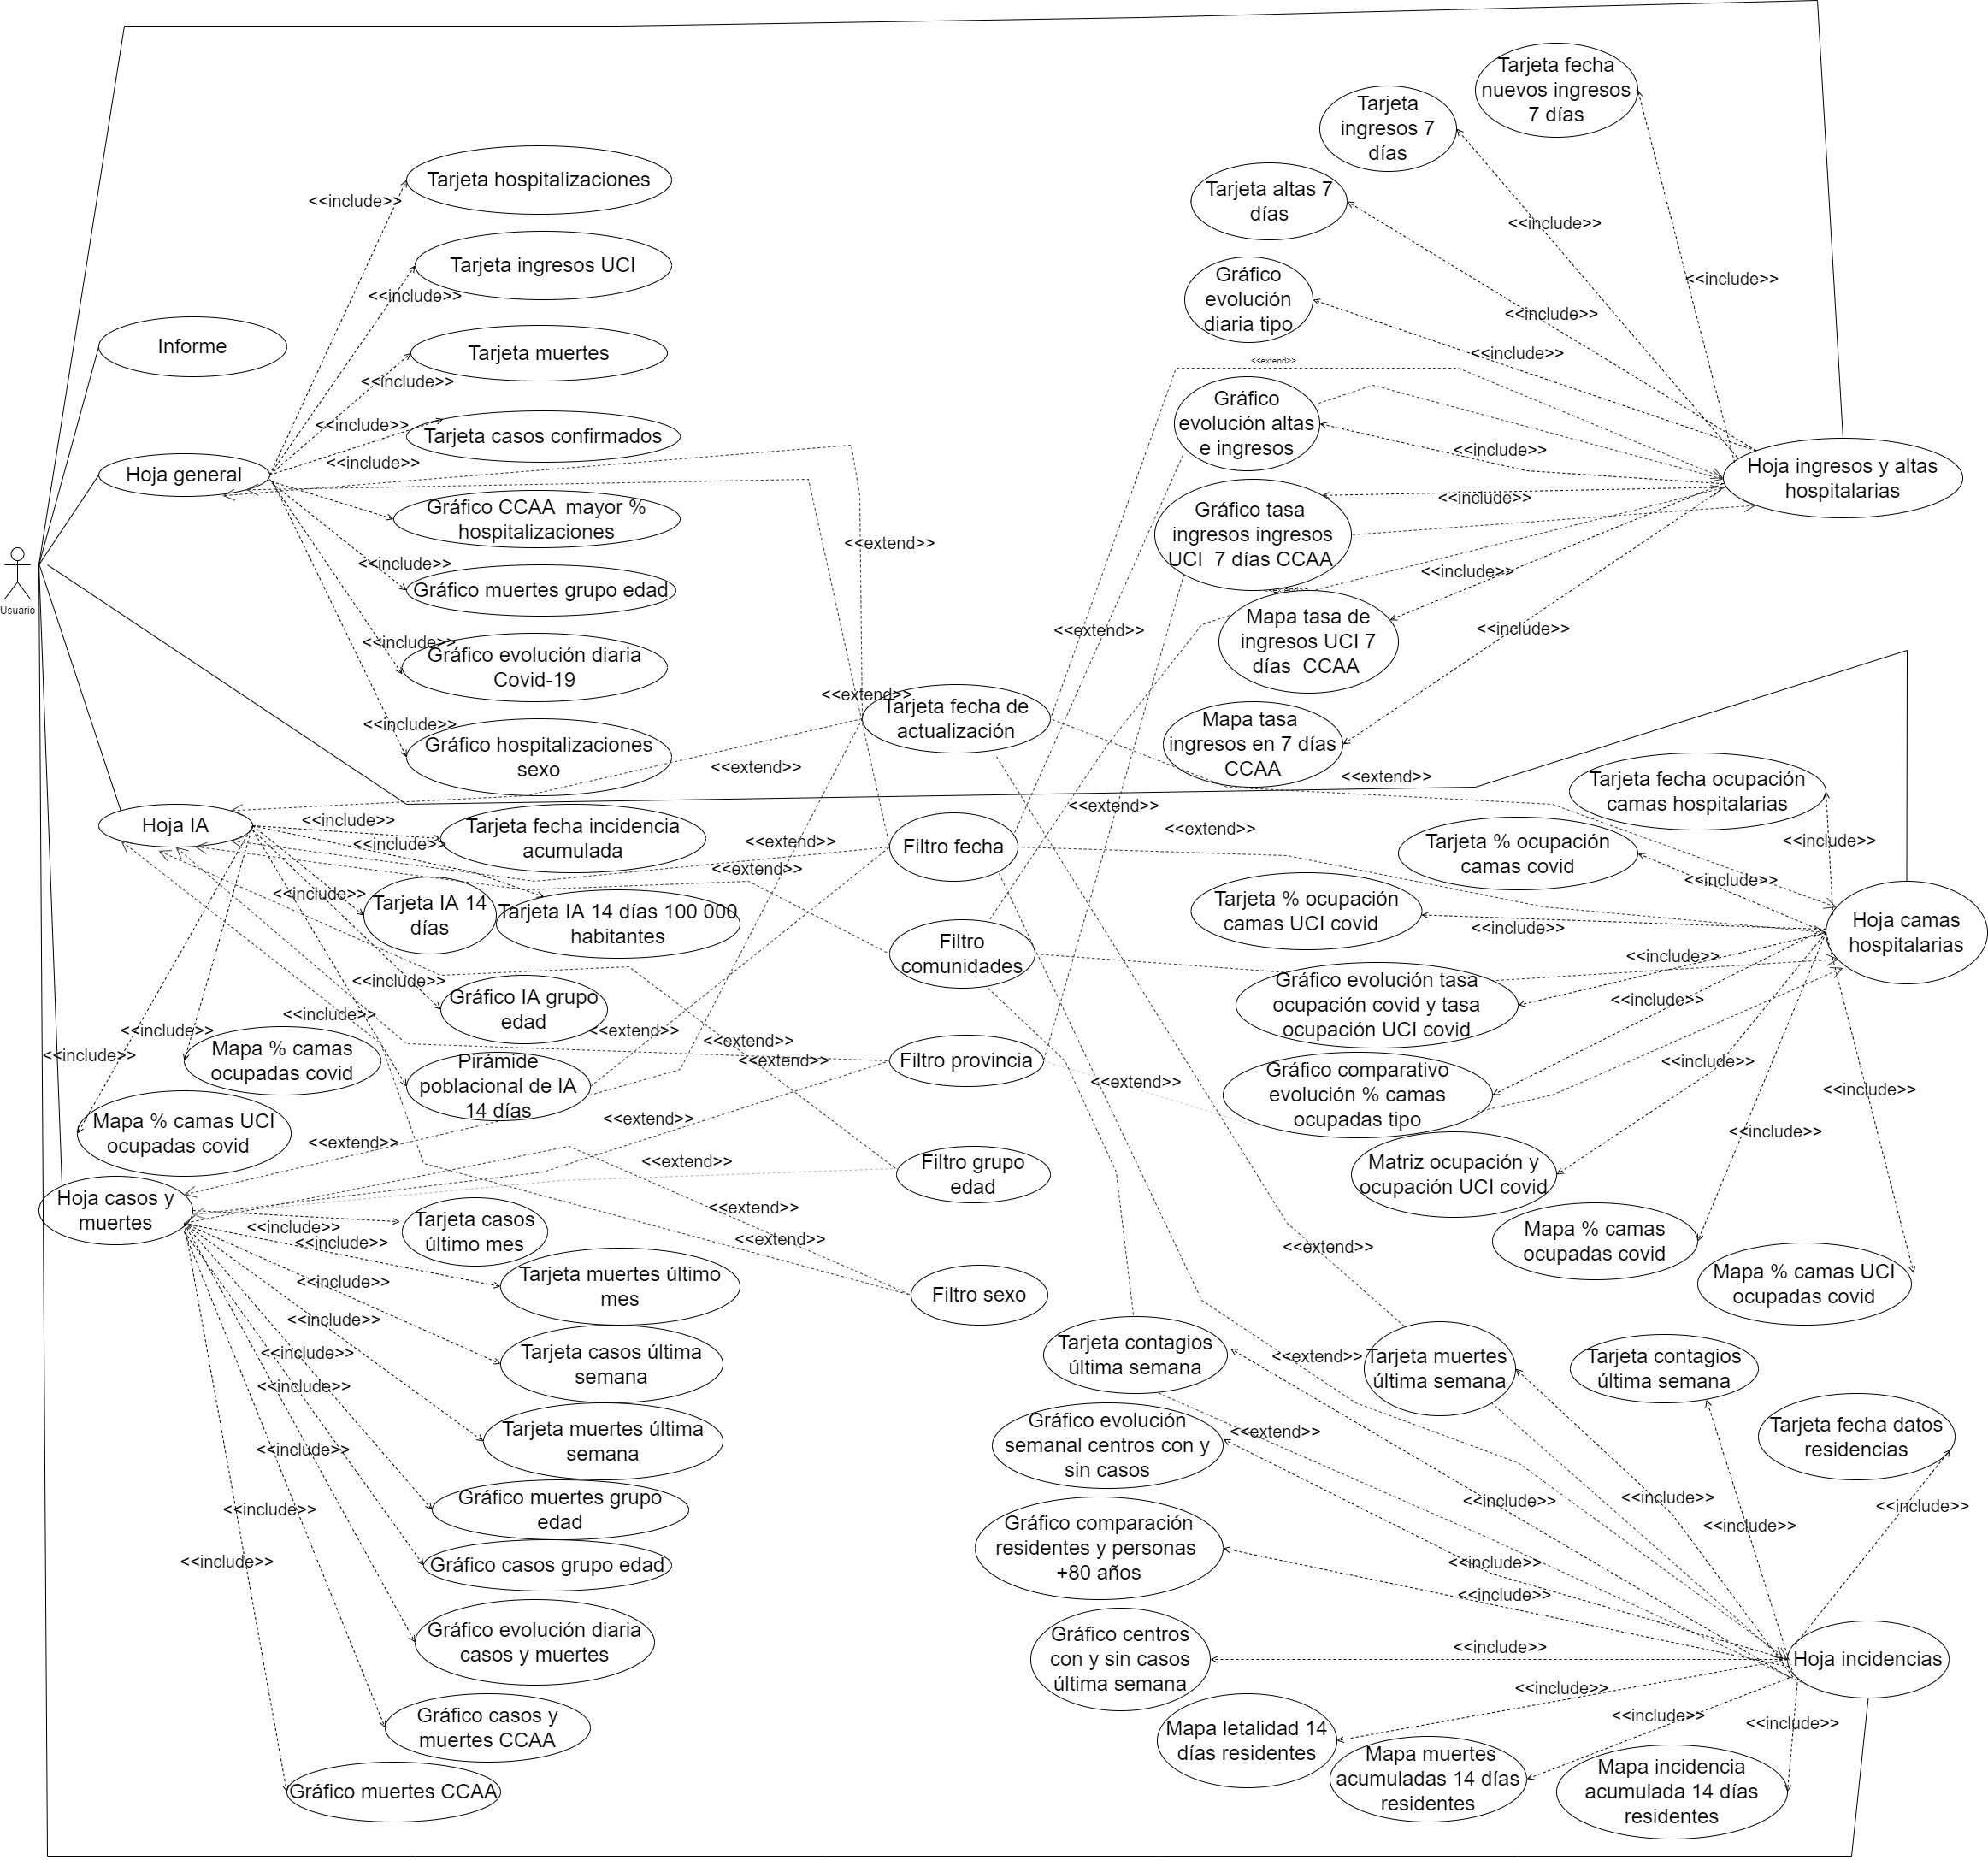
\includegraphics[scale=0.255]{img/diag2.drawio.png}
    \caption{Diagrama de casos de uso.}
\end{figure}



\apendice{Especificación de diseño}

\section{Introducción}
En esta parte del anexo se explica cómo se han organizado los elementos que componen la aplicación: sus datos, su arquitectura, sus interfaces, etc.
\section{Diseño de datos}
\subsection{Casos}
Se ha realizado un modelado dimensional en tres fases: modelo conceptual, modelo lógico y modelo físico.

Los modelos de casos se utilizan en distintas hojas del cuadro de mandos, como en el resumen, en la incidencia acumulada, y en casos y muertes.

\subsubsection{Modelo conceptual de casos}
El modelo conceptual de casos es el siguiente:

\imagen{casos_conc}{Modelo conceptual de casos.}

\subsubsection{Modelo lógico de casos}

El modelo lógico de casos es el siguiente:

\begin{figure}[h]
    \advance\leftskip-0.5cm \rightskip5cm
    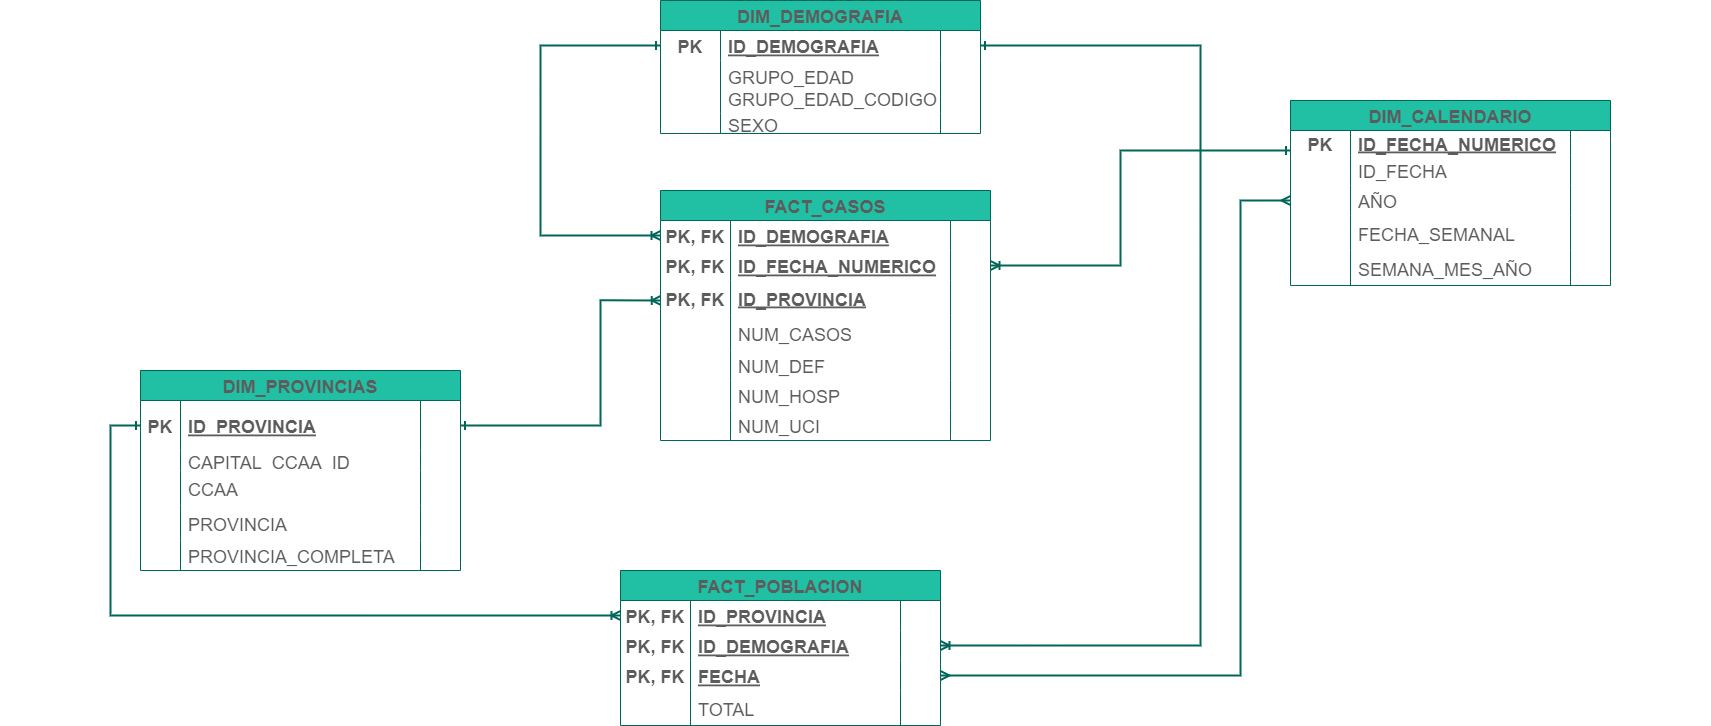
\includegraphics[scale=0.25]{img/casos_logico.png}
    \caption{Modelo lógico de casos.}
\end{figure}
\newpage

\subsubsection{Modelo físico de casos}
El modelo físico de casos es el siguiente:

\begin{figure}[h]
    \advance\leftskip-0.5cm \rightskip5cm
    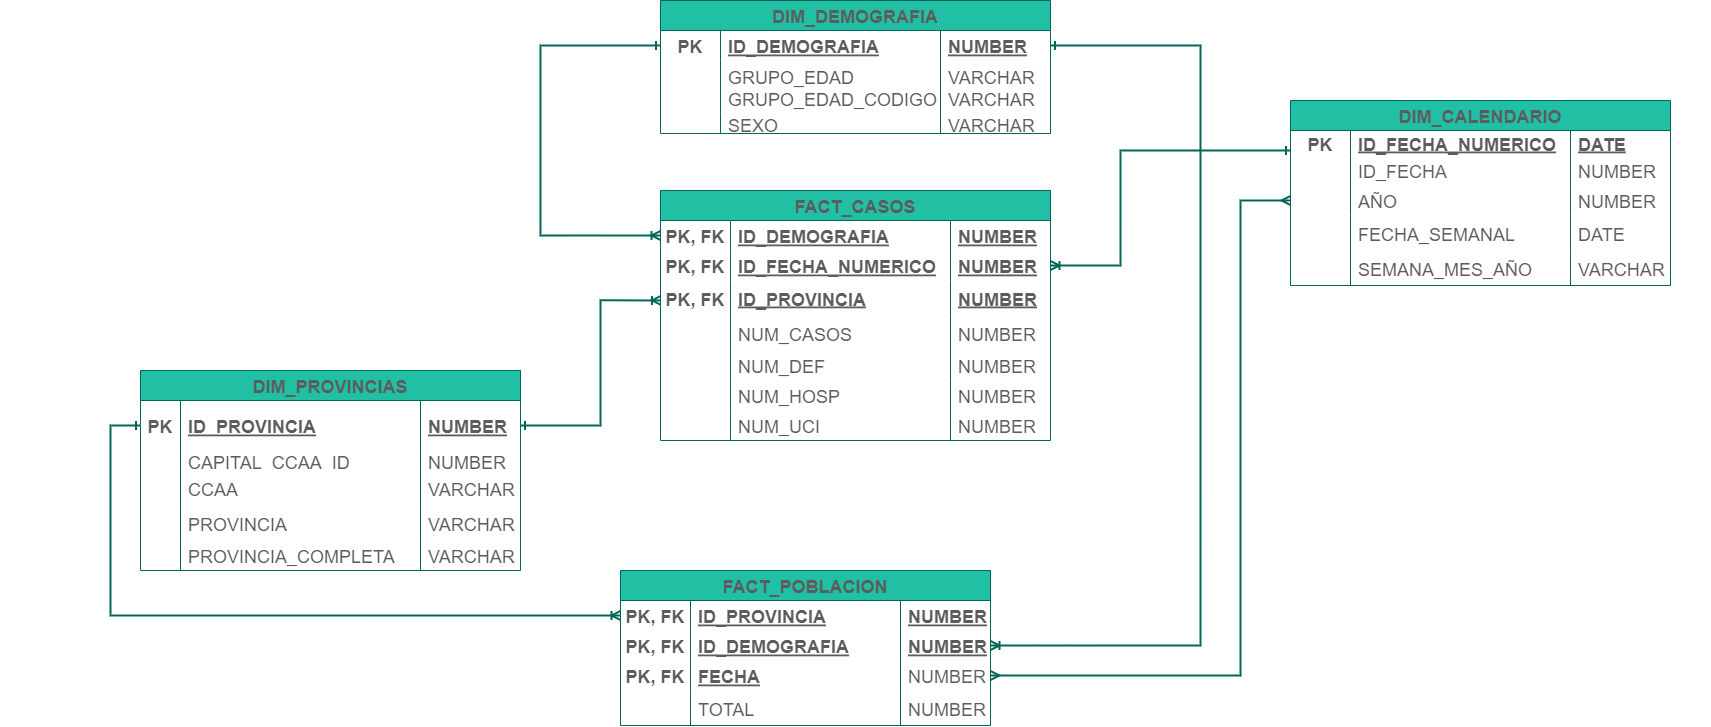
\includegraphics[scale=0.25]{img/casos_fisico.png}
    \caption{Modelo físico de casos.}
\end{figure}

\subsection{Hospitales}
Se ha realizado un modelado dimensional en tres fases: modelo conceptual, modelo lógico y modelo físico.

Los modelos de hospitales se utilizan en distintas hojas del cuadro de mandos, como en ingresos y altas hospitalarias, y camas hospitalarias.

\subsubsection{Modelo conceptual de hospitales}
El modelo conceptual de hospitales es el siguiente:

\imagen{hospitales_conc}{Modelo conceptual de hospitales.}

\subsubsection{Modelo lógico de hospitales}
El modelo lógico de hospitales es el siguiente:

\begin{figure}[h]
    \advance\leftskip-2cm \rightskip5cm
    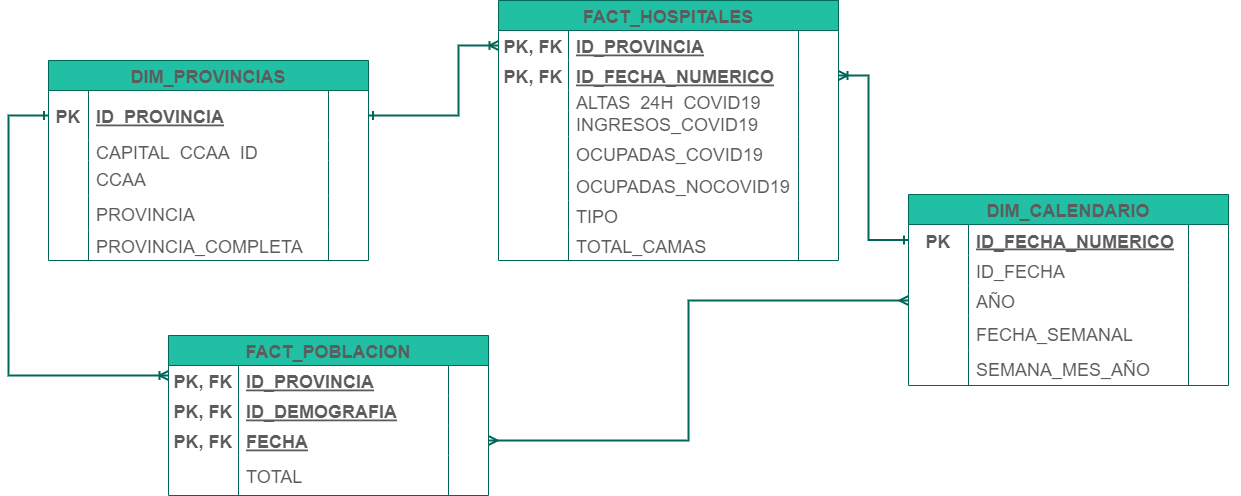
\includegraphics[scale=0.65]{img/hospitales_logico.png}
    \caption{Modelo lógico de hospitales.}
\end{figure}
\newpage

\subsubsection{Modelo físico de hospitales}
El modelo físico de hospitales es el siguiente:
\begin{figure}[h]
    \advance\leftskip-1cm \rightskip5cm
    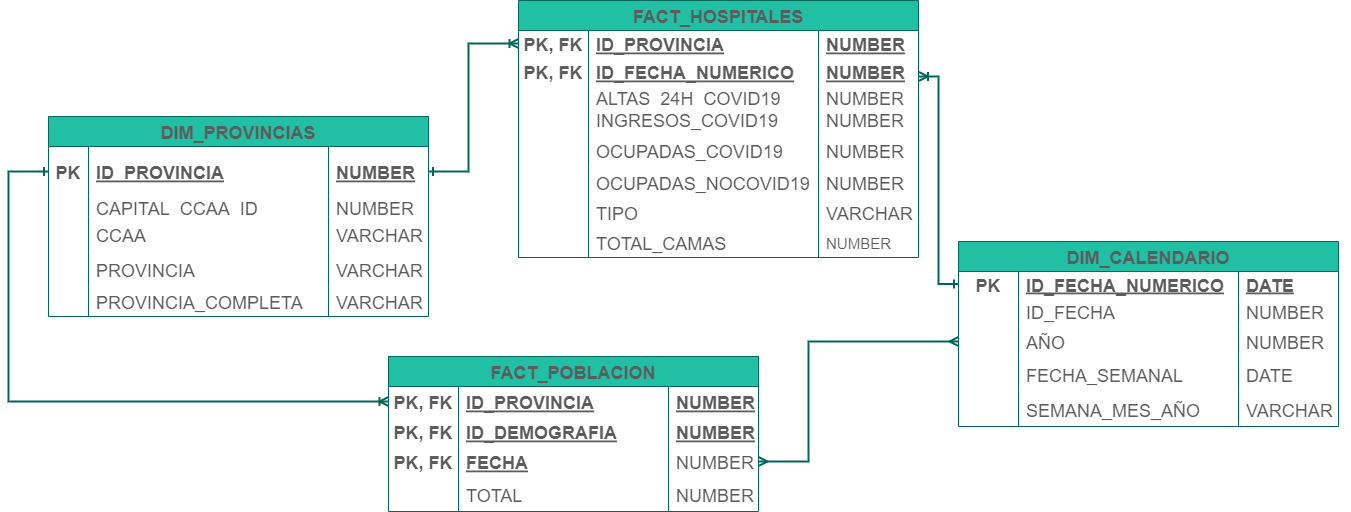
\includegraphics[scale=0.6]{img/hospitales_fisico.png}
    \caption{Modelo físico de hospitales.}
\end{figure}

\subsection{Residencias}
Se ha realizado un modelado dimensional en tres fases: modelo conceptual, modelo lógico y modelo físico.

Los modelos de residencias se utilizan la hoja del cuadro de mandos de residencias.

\subsubsection{Modelo conceptual de residencias} El modelo conceptual de residencias es el siguiente:
\imagen{residencias_conc}{Modelo conceptual de residencias.}

\subsubsection{Modelo lógico de residencias}
El modelo lógico de residencias es el siguiente:

\begin{figure}[h]
    \advance\leftskip-1.5cm \rightskip5cm
    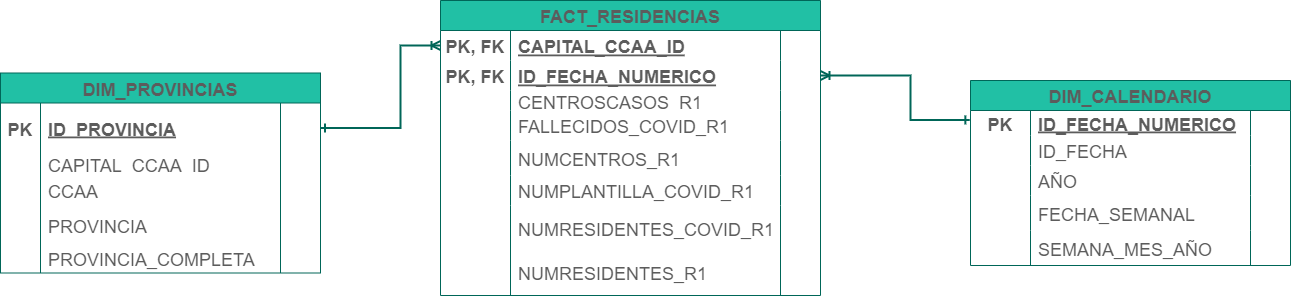
\includegraphics[scale=0.6]{img/residencias_logico.png}
    \caption{Modelo lógico de residencias.}
\end{figure}

\subsubsection{Modelo físico de residencias}
El modelo físico de residencias es el siguiente:

\begin{figure}[h]
    \advance\leftskip-0.5cm \rightskip5cm
    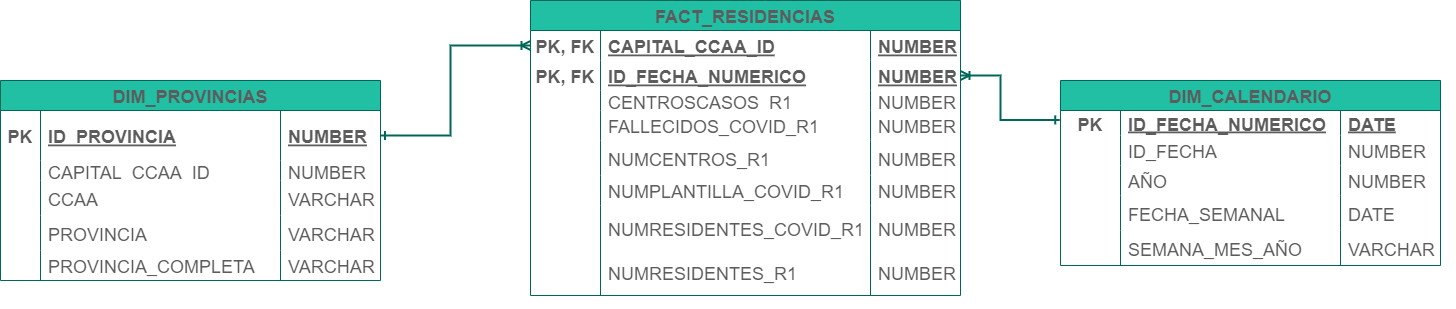
\includegraphics[scale=0.5]{img/residencias_fisico.png}
    \caption{Modelo físico de residencias.}
\end{figure}
\newpage

\subsection{Modelo final}
De esta forma el modelo final obtenido se compone de:

\begin{itemize}
    \item Casos: en esta tabla se almacena el número de casos, el número de defunciones, el número de hospitalizaciones y el número de casos en la UCI. Estos datos vienen agrupados en las siguientes columnas: identificador de demografía, identificador de fecha, identificador de provincia. Es una tabla de hechos, por lo tanto, se usarán sus datos para realizar cálculos.
    \item Provincias: en esta tabla se almacenan todas las provincias de España, cada provincia tiene los siguientes campos: el identificador de cada provincia, el código ISO de la provincia, la comunidad autónoma a la que pertenece, el código de la comunidad autónoma que pertenece y la respectiva capital de esa comunidad autónoma. Esta tabla es una dimensión y, por tanto, se usará para filtrar los cálculos que se hagan con las tablas de hecho.
    \item Demografía: en esta tabla se almacenan los datos demográficos, específicamente, el sexo y el grupo de edad, por tanto, esta tabla contará con los siguientes campos: el identificador de demografía, el grupo de edad y sexo. Esta tabla es una dimensión y por tanto se usará para filtrar los cálculos que se hagan con las tablas de hecho.
    \item Calendario: en esta tabla se almacenan las fechas de los datos contenidos en alguna de las tablas de hecho. Los campos de esta tabla son: el identificador de fecha y año, la fecha, el día de la semana, el día, el mes, el mes y año, el mes y año de forma numérica, la semana, la semana y mes, el trimestre, el trimestre y año, y el mes de forma numérica. Esta tabla es una dimensión y, por tanto, se usará para filtrar los cálculos que se hagan con las tablas de hecho.
    \item Población: en esta tabla se almacenan los datos sobre la población y está agrupada mediante las siguientes columnas: el identificador de demografía, el identificador del año, el identificador de la provincia. Es una tabla de hechos, por lo tanto, se usarán sus datos para realizar cálculos.
    \item Hospitales: en esta tabla se almacenan los datos sobre la situación en los hospitales: el número de altas en Covid-19 en las últimas 24 horas, el número de ingresos por Covid-19, el número de camas ocupadas por Covid-19, el tipo de hospitalización, el número total de camas en el hospital correspondiente, agrupados por el identificado de fecha y el identificador de provincia. Es una tabla de hechos, por lo tanto, se usarán sus datos para realizar cálculos.
    \item Residencias: en esta tabla se almacenan los datos sobre la situación en las residencias:  el número de centros, el número de plantilla Covid-19, el número de residentes con Covid-19, y el número de residentes, agrupadas por el identificador de fecha y el identificador de la capital de la comunidad autónoma.
\end{itemize}

\begin{figure}[h]
    \advance\leftskip-2cm \rightskip5cm
    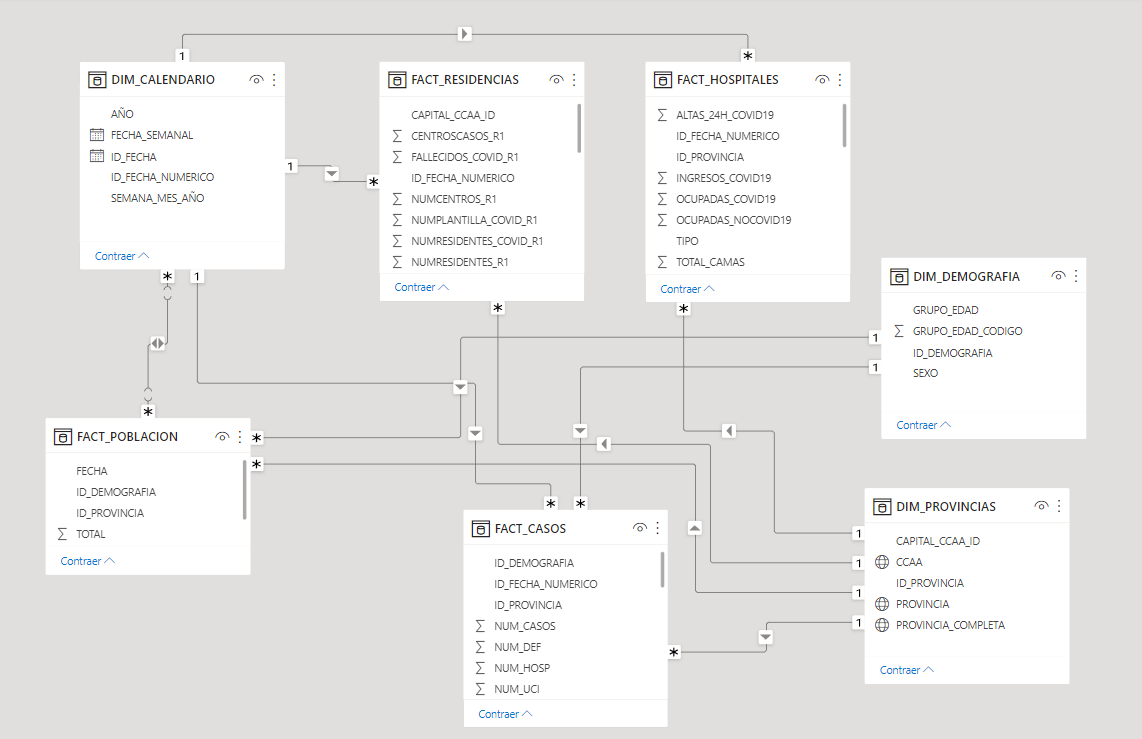
\includegraphics[scale=0.7]{img/modelo-final.PNG}
    \caption{Modelo final.}
\end{figure}
\section{Diseño procedimental}
En esta parte del anexo se muestra la ejecución de la arquitectura mediante diagramas de secuencia principalmente.

\subsection{Extracción}
Este primer diagrama de secuencia representa el proceso de extracción de los datos, desde su fuente hasta el data lake, donde se realizará la carga de los datos.
\imagen{extracción}{Diagrama de secuencia de extracción de datos.}

\subsection{Carga}
Este diagrama de secuencia representa el proceso de carga de los datos desde el data lake hasta la data warehouse Snowflake, concretamente su base de datos RAW.
\imagen{carga}{Diagrama de secuencia de carga de datos.}

\subsection{Transformación}
Este diagrama de secuencia representa el proceso de transformación dbt, en el que se recogen los datos crudos desde Snowflake, desde la base de datos RAW, realiza las transformaciones y los carga de nuevo en Snowflake, en la base de datos ANALYTICS.
\imagen{transformación}{Diagrama de secuencia de transformación de datos.}
\subsubsection{DAG transformaciones dbt}
A continuación, se muestra el Grafo Dirigido Acíclico (DAG) mediante el cual hace dbt las transformaciones de sus modelos.

\begin{landscape}
\begin{figure}[h]
    \advance\leftskip-1.5cm \rightskip5cm
    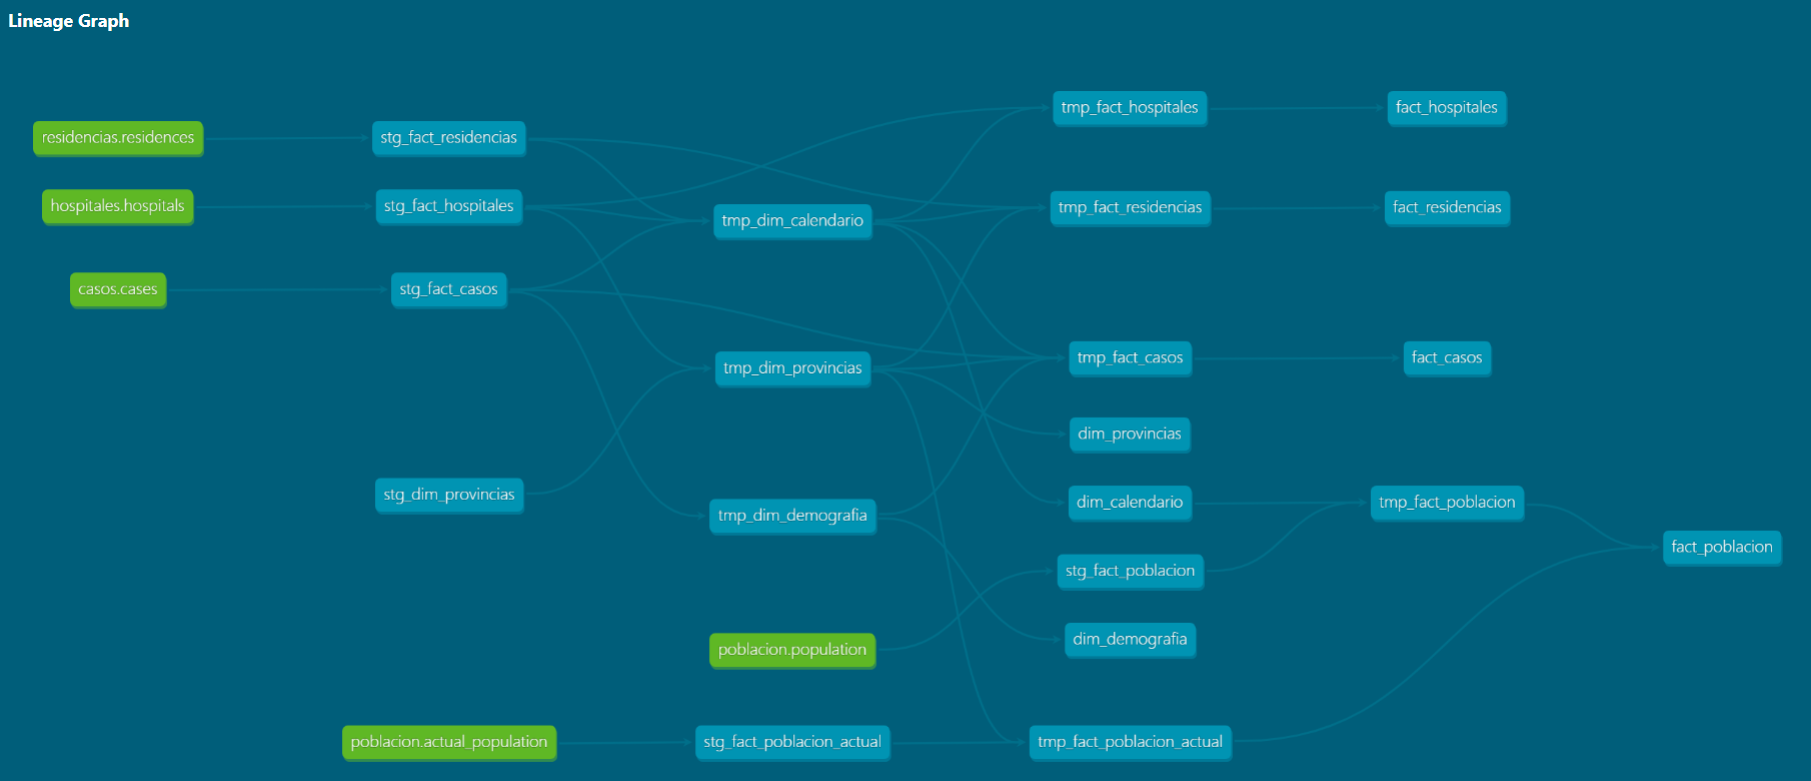
\includegraphics[scale=0.6]{img/DAG.PNG}
    \caption{Grafo Dirigido Acíclico (DAG) de las transformaciones.}
\end{figure}
\end{landscape}  

\subsection{Conexión de PowerBI a Datawarehouse}
Este diagrama de secuencia representa el proceso de conexión de PowerBI a snowflake, concretamente su base de datos ANALYTICS, mediante la cual se mantienen actualizados los datos en su cuadro de mandos.

\imagen{conexión}{Diagrama de secuencia de conexión de PowerBI a Datawarehouse.}

\subsection{Visualización de los datos por el usuario}
Este diagrama de secuencia representa el proceso de visualización de los datos por el usuario, y los pasos que este sigue.

\imagen{visualización}{Diagrama de secuencia de visualización de datos.}

\section{Diseño arquitectónico}

En este apartado se explicará el tipo de arquitectura que se ha escogido y que se ha seguido para tener un buen diseño.

\subsection{\emph{Modern Data Stack}}
Los Modern Data Stack \cite{Modern_Data_Stack} toman ventaja de los data warehouses en la nube, ya que traen mejoras en seguridad y elasticidad, y principalmente en el almacenamiento y procesamiento de grandes volúmenes de datos a gran velocidad y un coste muy bajo.

Los data warehouses solían ser un gran cuello de botella. Se usaban principalmente bases de datos relacionales basadas en filas como sus data warehouses, lo que no se adaptaba bien a las cargas de trabajo de análisis de datos, ya que distribuye los datos relacionados en varios discos o servidores. Incluso con tecnologías como Hadoop tardaban horas en ejecutarse y eran muy complicados de escribir y mantener. 

Además, debido al limitado poder de procesado de las antiguas data warehouses los ingenieros de datos solían hacer el trabajo de transformación antes de cargar los datos, lo que dio lugar al término ETL (\emph{Extract-Transform-Load}).

Ahora, con el avance de los data warehouse en la nube, gracias a su alto rendimiento, los ingenieros de datos pueden ejecutar consultas a escala de petabytes en minutos. 

Con un \emph{Modern Data Stack}, se pueden cargar los datos en el data warehouse en minutos y la transformación de datos se puede manejar de manera mucho más efectiva allí que en alguna capa de procesamiento externa (ELT, \emph{Extract-Load-Transform}).

Los princiapes beneficios de un Modern Data Stack por lo tanto son:

\begin{itemize}
	\item Modularidad: debido a que los Modern Data Stack consisten en varias tecnologías con puntos de conexión general, se pueden cambiar partes del stack a medida que las necesidades cambian, lo que ayuda a evitar el vendor lock-in.
	\item Velocidad: debido a los límites de procesamiento de las antiguas data warehouses, los pipelines podían llegar a tardar horas en ejecutarse, pero ahora con el Modern Data Stack y sus recursos de cómputo elásticos, ese trabajo puede hacerse en minutos.
	\item Coste: los costes de la tecnología en la nube son normalmente significativamente más baratos que su contraparte on-premise. Un data warehouse antiguo tendría que pagar por un servidor todo el tiempo, aparte de ser costoso y disponer de dificultades en su escalabilidad, al contrario que con un data warehouse en la nube, donde solo pagas por lo que usas y puedes escalar para cargas de trabajo masivas cuando sea necesario.
\end{itemize}

\subsection{ELT}
Los procesos ELT (\emph{Extract, load and transform}) \cite{ELT} consisten en la extracción, carga y transformación de datos. 

De manera que se diferencian de los procesos ETL en que los datos no se transforman al obtener los datos, sino que se guardan antes de ser procesados, es decir son almacenados en su formato inicial.

Esta nueva perspectiva está compuesta por:

\subsubsection{Modern ingestion}
La ingestión de datos \cite{Modern} comprende las fases de extracción de datos desde la fuente y la carga de estos mismo en el destino, la E y L del proceso ETL.

\subsubsection{Modern Storage}
El almacenamiento de datos \cite{Modern} se realiza mediante almacenes de datos en la nube, entre los que se incluyen \emph{Snowflake}.

Actualmente, estos almacenes de datos modernos presentan una serie de mejoras respecto a los anteriores, ya que permiten la ausencia de configuraciones de \emph{hardware}, y se caracterizan por su disponibilidad, rapidez y menor coste.

\subsubsection{Modern transformation}
La transformación moderna de datos \cite{Modern} convierte, limpia y agrega, entre otras funciones, los datos. Y todas estas acciones se realizan directamente sobre el data warehouse analítico.


\subsection{Aplicación en el proyecto}

Para el proyecto se ha construido la siguiente arquitectura:

\subsubsection{Ingestión de datos}

La primera parte de la arquitectura del Modern Data Stack es la ingestión, correspondiente al EL, la extracción y carga de datos, del ELT. Para ello se han utilizado varias herramientas, ya que tenemos varias fuentes de datos que hay actualizar frecuentemente como los datos de los casos, los datos hospitalarios, etc. Hemos montado una estructura capaz de extraer y cargar los datos diaria y automáticamente, de forma que siempre tengamos lo datos actualizados. Estas herramientas son las siguientes:

\begin{itemize}
	\item Google cloud: \cite{google_cloud} es un espacio virtual por el que se puede realizar una serie de tareas que antes requerían de hardware o software, y que ahora usan la nube de Google como única forma de acceso, almacenamiento y gestión de datos. Especificamente se han utilizado los siguientes servicios:
	\begin{itemize}
    	\item Cloud functions: \cite{cloud_functions} es un servicio que sirve para crear aplicaciones sin servidores dentro de Google Cloud, dando respuesta a la demanda de eventos que puedan ocurrir en cualquier sitio. Lo positivo de este servicio es que abonarás solo por lo que uses, ósea el tiempo que tu código se esté ejecutando, por lo tanto, es buena opción para proyectos pequeños. En este caso lo hemos utilizado para realizar un script de Phyton \cite{Python} que extrae desde URLs de fuentes oficiales del estado, .csv con los datos que queremos actualizar diariamente de la pandemia para llevarlos a Amazon S3, nuestro data lake, dónde reunimos los datos antes de cargarlos en nuestro data warehouse.
    	\item Cloud Scheduler: \cite{cloud_scheduler} es un programador de trabajos cron administrado. Permite programar prácticamente cualquier trabajo, desde trabajos por lotes y de macrodatos, hasta operaciones de infraestructura de nube y mucho más. Es el servicio que usamos para que se ejecuten nuestros scripts de phyton de forma diaria.
    	\item Pub|Sub: \cite{pub/sub} este servicio permite que otros servicios se comuniquen de forma asíncrona. Se usa para las canalizaciones de integración de datos y estadísticas de transmisión a fin de transferir y distribuir datos. Es igual de efectivo que un middleware orientado a la mensajería para la integración de servicio, o como una cola a fin de paralelizar tareas. Lo usamos para que se pueda comunicar Cloud Scheduler con el script de python programado en Cloud functions.
    \end{itemize}
	\item Amazon S3: \cite{Amazon} es un servicio que ofrece el almacenamiento de elementos a partir de una interfaz de servicio web. Se puede almacenar cualquier tipo de objeto, por lo que se le puede dar varios usos. En nuestro caso será usado como un data lake. El script de python comentado en el apartado anterior, va a cargar en este data lake los .csv que queremos cargar en el data warehouse. 
	\item Fivetran: \cite{Fivetran} es una herramienta que permite a las compañías extraer datos de varias fuentes y cargarlas en un destino, normalmente un data warehouse en la nube. Estas tareas de integración están automatizadas y usan conectores de datos preconstruidos, que hay que configurar para que se conecten a las fuentes y el destino de los datos. En nuestro caso, lo usaremos para cargar nuestros datos del data lake creado en Amazon S3 en nuestra datewarehouse en Snowflake. Esta tarea también está automatizada, realizándose de manera diaria, de forma que tendremos siempre los datos actualizados. 

\end{itemize}

\subsubsection{Almacenamiento de datos}

Para almacenar los datos se ha utilizado la datawarehouse en la nube snowflake \cite{Snowflake}, la cual utiliza un repositorio de datos centralizado para datos persistentes, accesible desde todos los nodos del data warehouse, y que cuando va a procesar las consultas cada clúster almacena una porción de los datos localmente para procesarlos en paralelo.

En nuestro caso vamos a tener dos bases de datos. Una llamada RAW, con el esquema COVID, donde se cargarán desde Amazon S3 los datos crudos. Y otra llamada ANALYTICS dónde estarán los datos transformados. Esta base de datos tendrá dos esquemas, DBT\_JOSEDANIELBALLESTER, donde se cargarán los datos desde entorno de desarrollo, y el esquema ANALYTICS, donde se cargarán los datos del entorno de producción, desde el cual se cargará posteriormente a PowerBI para su explotación.

La arquitectura de Snowflake tiene 3 capas:

\begin{itemize}
	\item Database storage: en esta capa están los datos, una vez están en la nube, Snowflake los reorganiza en su propio formato para mejorar el rendimiento.
	\item Query processing: esta capa realiza las consultas mediante almacenes virtuales, cada uno de ellos es un cluster de varios nodos que trabajan en paralelo.
	\item Cloud services: son varios servicios que coordinan las actividades de Snowflake.
\end{itemize}

\subsubsection{Transformación de datos}

Para la transformación utilizaremos dbt, el cual se conectará con Snowflake, cogerá los datos desde la base de datos RAW y una vez realizadas las transformaciones, cargará los datos en la base de datos ANALYTICS.

Dbt \cite{dbt} es una herramienta de línea de comandos que permite desarrollar colaborativamente código de analítica. Es la herramienta que se encarga de las trasformaciones, la T del ELT, siguiendo las mejores prácticas de la ingeniería del software como la modularidad, portabilidad, la integración y distribución continua, la documentación, el control de versiones, y el testeo de cada modelo, permitiendo construir data pipelines robustos.

Dbt depende de SQL para transformar los datos, no le queda más remedio ya que, al estar transformando los datos directamente en la data warehouse en la nube, está delegando todo el trabajo pesado en su motor. Aun así, dbt agrega funcionalidad de código como por ejemplo bucles, que no hay en SQL, gracias al template jinja, lo que permite escribir código más eficiente.

En su flujo de trabajo para las transformaciones se generan automáticamente grafos de dependencia y su ejecución se puede programar y automatizar en su entorno en la nube, cosa que se ha hecho, de forma que diariamente se van a realizar las transformaciones programadas sobre la base de datos RAW, cargándolas en la base de datos ANALYTICS, de forma que PowerBI tendrá siempre datos actualizados, de cómo mucho un día de antigüedad disponibles.

\subsubsection{Reporting}

Microsoft Power BI\cite{MPBI} es una herramienta que posibilita la conexión a distintas fuentes de datos locales o en la nube. De forma que se puede ajustar la información fácilmente, permitiendo producir tableros de control en tiempo real, e informes que incluyen la información óptima para la mejora del desarrollo de los resultados.
	
Así, Microsoft Power BI permite unir diferentes fuentes de datos, modelizar y analizar datos para después, presentarlos a través de paneles e informes; y que así puedan ser consultados de una manera fácil, atractiva e intuitiva.
	
Por ello, es una herramienta usada para la fase de análisis y creación de paneles e informes, que permite realizar diversos gráficos que ayudan a visualizar los datos y sacar insights de forma cómoda y flexible gracias a la posibilidad de aplicar filtros dinámicos.

Nuestro panel va a estar alojado en la nube, de forma que va a ser posible acceder a él a través de una URL, además al estar conectado directamente a Snowflake, hemos programado que de forma diaria se actualice automáticamente cargando los datos alojados en la base de datos ANALYTICS.

\begin{figure}[h]
    \advance\leftskip-2cm \rightskip5cm
    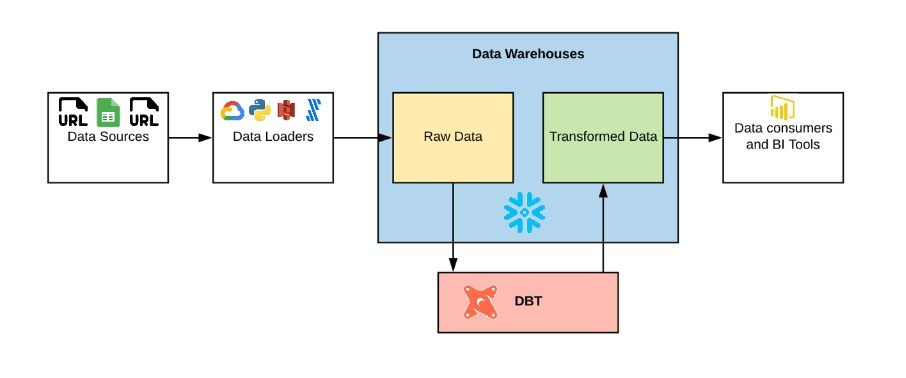
\includegraphics[scale=0.55]{img/dis_arq.jpeg}
    \caption{Diseño arquitectónico.}
\end{figure}

\section{Diseño de interfaces}
Para la realización del proyecto, primero se desarrolló un prototipo de las diferentes interfaces del cuadro de mandos con la herramienta de diseño Canva. De esta forma se asentaron las ideas de cómo iba a ser el diseño del cuadro de mandos en un principio.

\newpage
El primero que se diseñó fue el prototipo resumen de la situación general de Covid-19. 

\begin{figure}[h]
    \advance\leftskip-1cm \rightskip5cm
    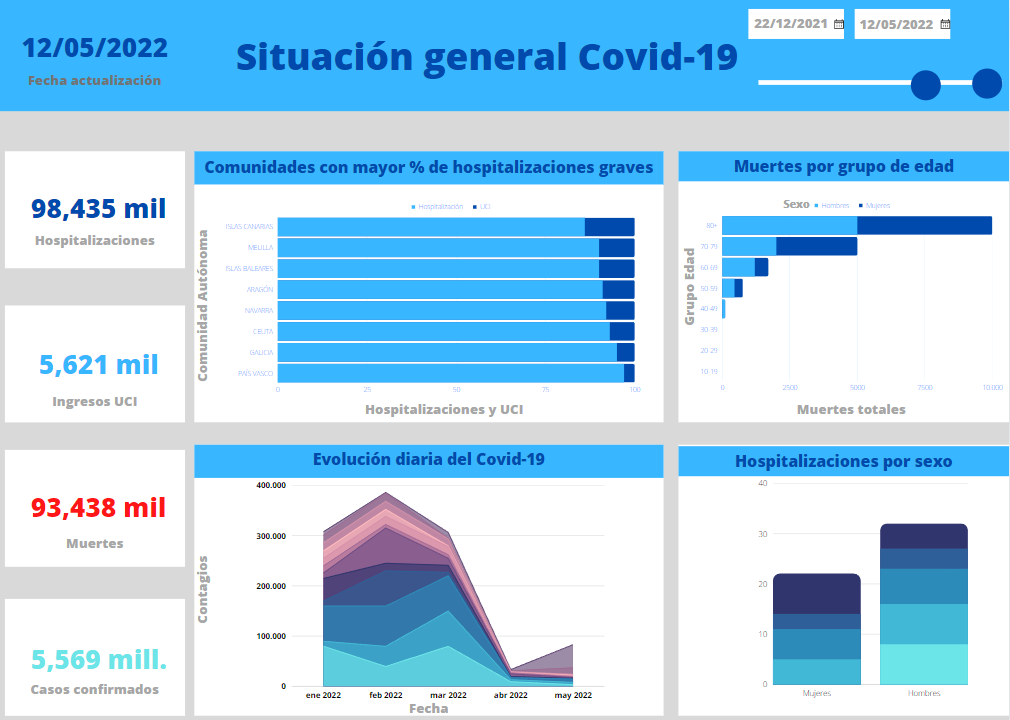
\includegraphics[scale=0.7]{img/prototipo_resumen.PNG}
    \caption{Prototipo resumen.}
\end{figure}

Éste constaría de cinco tarjetas con datos sobre la fecha de actualización, hospitalizaciones, ingresos UCI, muertes, y casos confirmados. 

También, constaría de cuatro gráficos principales que facilitarían la visualización de información sobre las comunidades con mayor porcentaje de hospitalizaciones graves, las muertes por grupo de edad, la evolución diaria del Covid-19, y las hospitalizaciones por sexo, respectivamente.

Además, permitiría el filtrado de la información mediante un filtro de fecha.

\newpage
A continuación, se incluye la interfaz final del resumen de la situación general del Covid-19.

\begin{figure}[h]
    \advance\leftskip-0.5cm \rightskip5cm
    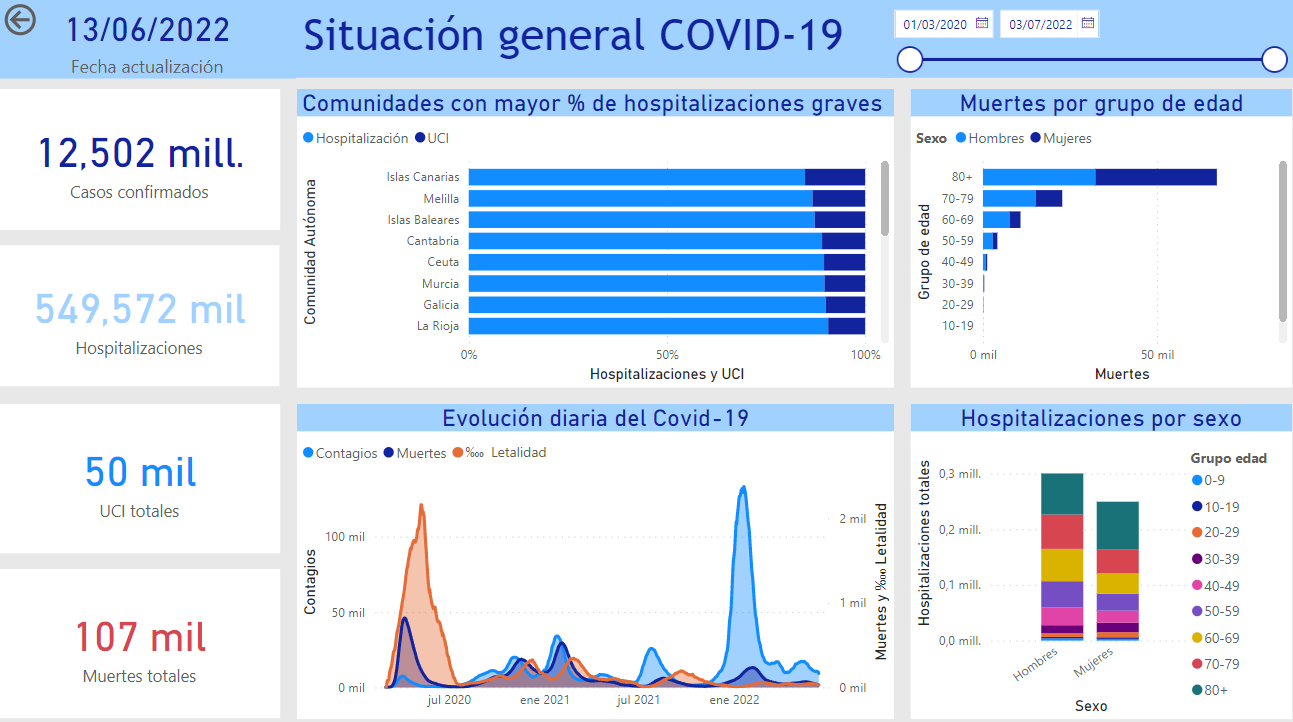
\includegraphics[scale=0.55]{img/powerBI_resumen.PNG}
    \caption{Diseño resumen.}
\end{figure}

Se puede ver como la interfaz final es prácticamente igual al prototipo inicial, por lo que se ha conseguido el correcto seguimiento del prototipo.

\newpage
Después, se diseñó el prototipo de la incidencia acumulada. 

\begin{figure}[h]
    \advance\leftskip-1cm \rightskip5cm
    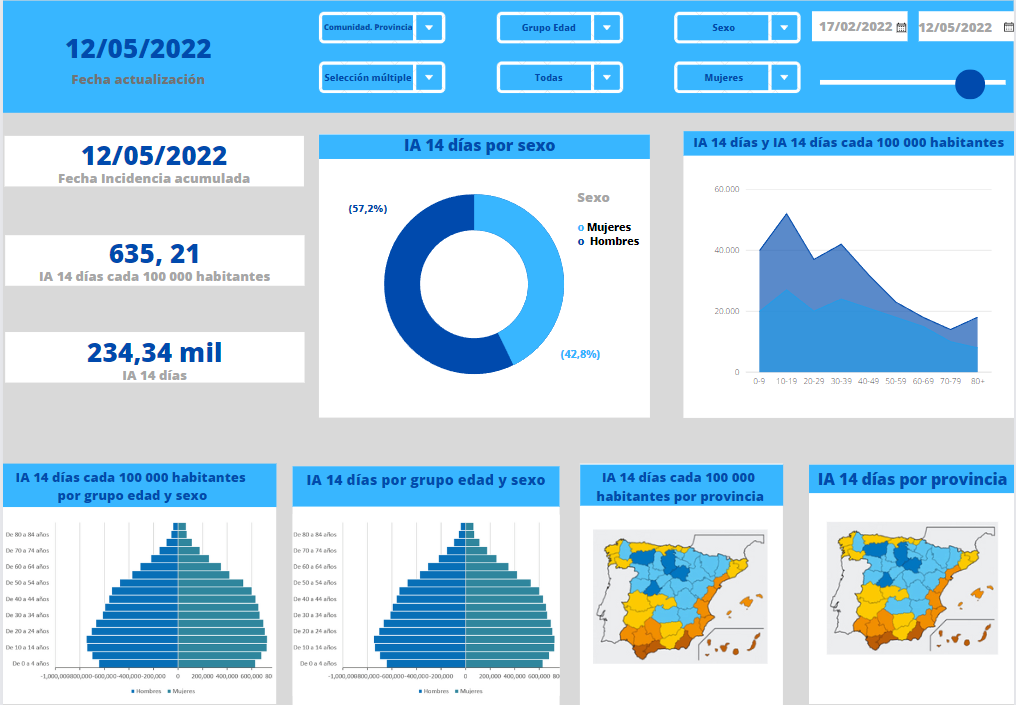
\includegraphics[scale=0.7]{img/prototipo_IA.png}
    \caption{Prototipo incidencia acumulada.}
\end{figure}

Éste constaría de cuatro tarjetas con datos sobre la fecha de actualización, la fecha de incidencia acumulada, la incidencia acumulada a 14 días cada 100.000 habitantes y la incidencia acumulada a 14 días. 

También constaría de cuatro gráficos y dos mapas  coropléticos, que facilitarían la visualización de información sobre la incidencia acumulada a 14 días por sexo, la incidencia acumulada a 14 días cada 100.000 habitantes, la incidencia acumulada a 14 días cada 100.000 habitantes por grupo de edad y sexo, la incidencia acumulada a 14 días por grupo de edad y sexo, la incidencia acumulada a 14 días cada 100.000 habitantes por provincia, y la incidencia acumulada a 14 días por provincia, respectivamente.

Además, permitiría el filtrado de la información mediante filtros de fecha, comunidades, provincia, grupo de edad y sexo.

\newpage
A continuación, se incluye la interfaz final de la incidencia acumulada. 

\begin{figure}[h]
    \advance\leftskip-0.5cm \rightskip5cm
    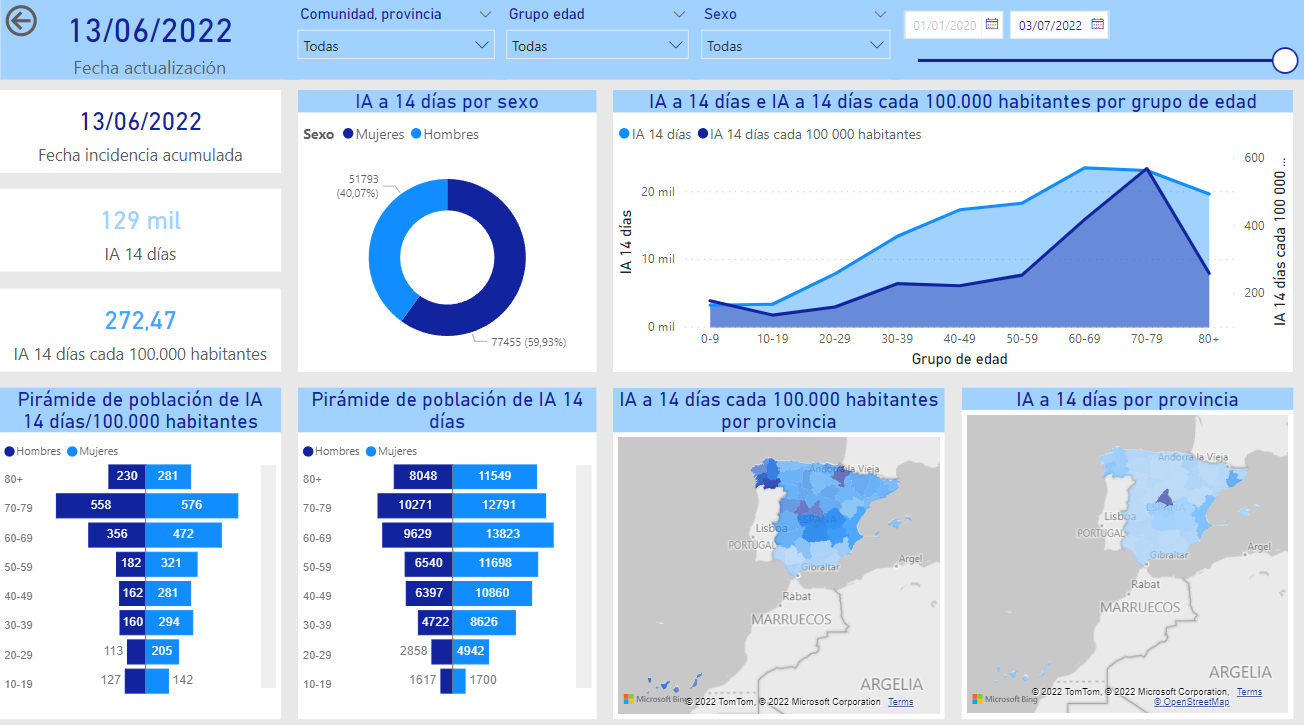
\includegraphics[scale=0.55]{img/powerBI_IA.PNG}
    \caption{Diseño incidencia acumulada.}
\end{figure}

A pesar de que la interfaz final es muy similar al prototipo inicial, difieren en una serie de aspectos como algún título de gráfico.

\newpage
Luego, se diseñó el prototipo de casos y muertes. 

\begin{figure}[h]
    \advance\leftskip-1cm \rightskip5cm
    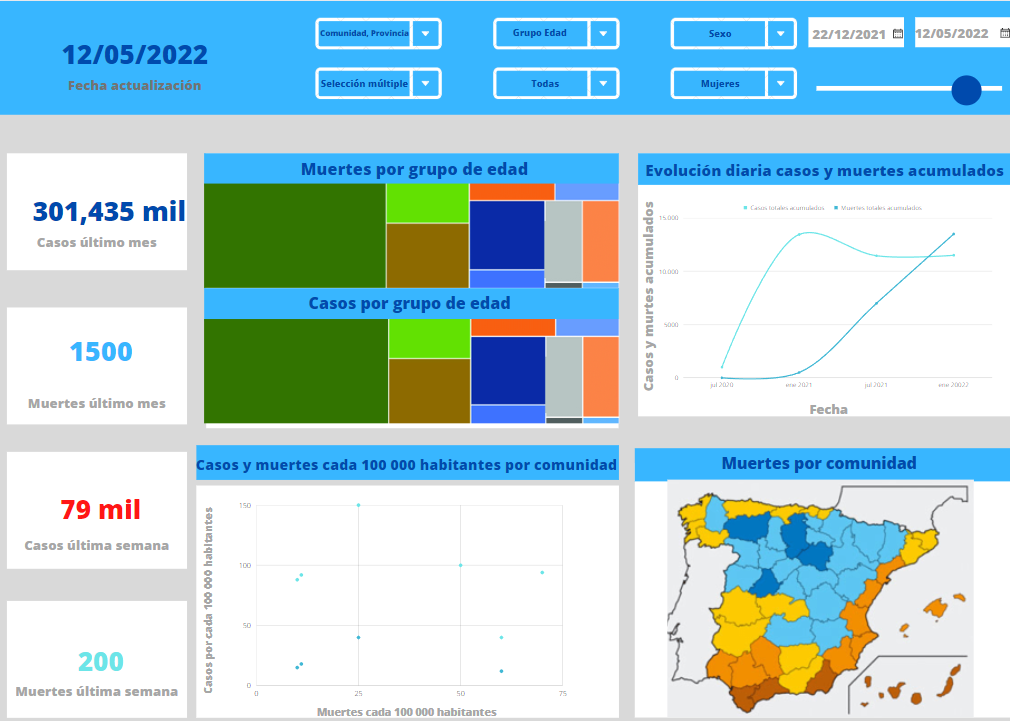
\includegraphics[scale=0.7]{img/prototipo_casosYmuertes.PNG}
    \caption{Prototipo casos y muertes.}
\end{figure}

Éste constaría de cinco tarjetas con datos sobre la fecha de actualización, los casos del último mes, las muertes del último mes, los casos de la última semana, y las muertes de la última semana. 

También constaría de tres gráficos y un mapa coroplético, que facilitarían la visualización de información sobre las muertes por grupo de edad, los casos por grupo de edad, la evolución diaria de los casos y muertes acumuladas, los casos y muertes cada 100.000 habitantes por comunidad, y las muertes por comunidad, respectivamente.

Además, permitiría el filtrado de la información mediante filtros de fecha, comunidades, provincia, grupo de edad y sexo.

\newpage 
A continuación, se incluye la interfaz final de los casos y muertes. 

\begin{figure}[h]
    \advance\leftskip-0.5cm \rightskip5cm
    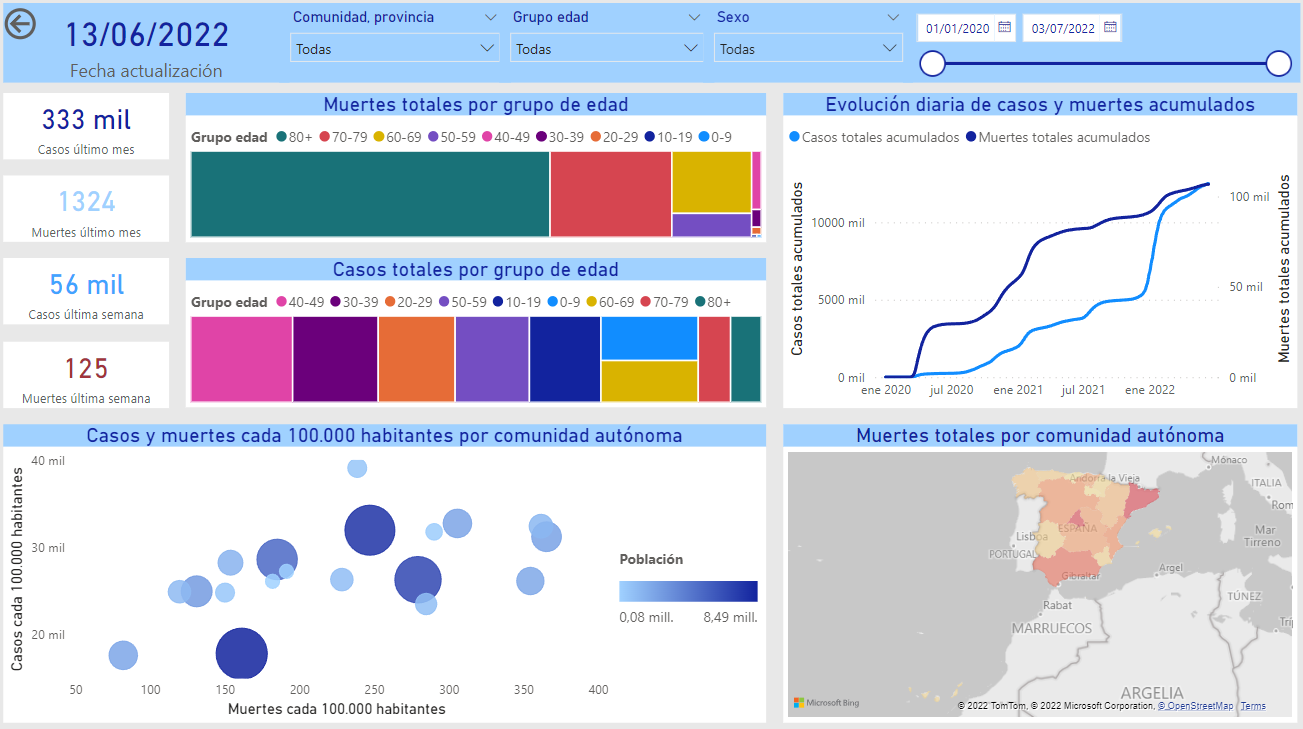
\includegraphics[scale=0.55]{img/powerBI_casosYmuertes.PNG}
    \caption{Diseño casos y muertes.}
\end{figure}

A pesar de que la interfaz final es muy similar al prototipo inicial, difieren en una serie de aspectos como algún título de gráfico.

\newpage
Posteriormente, se diseñó el prototipo de ingresos y altas hospitalarias. 

\begin{figure}[h]
    \advance\leftskip-1cm \rightskip5cm
    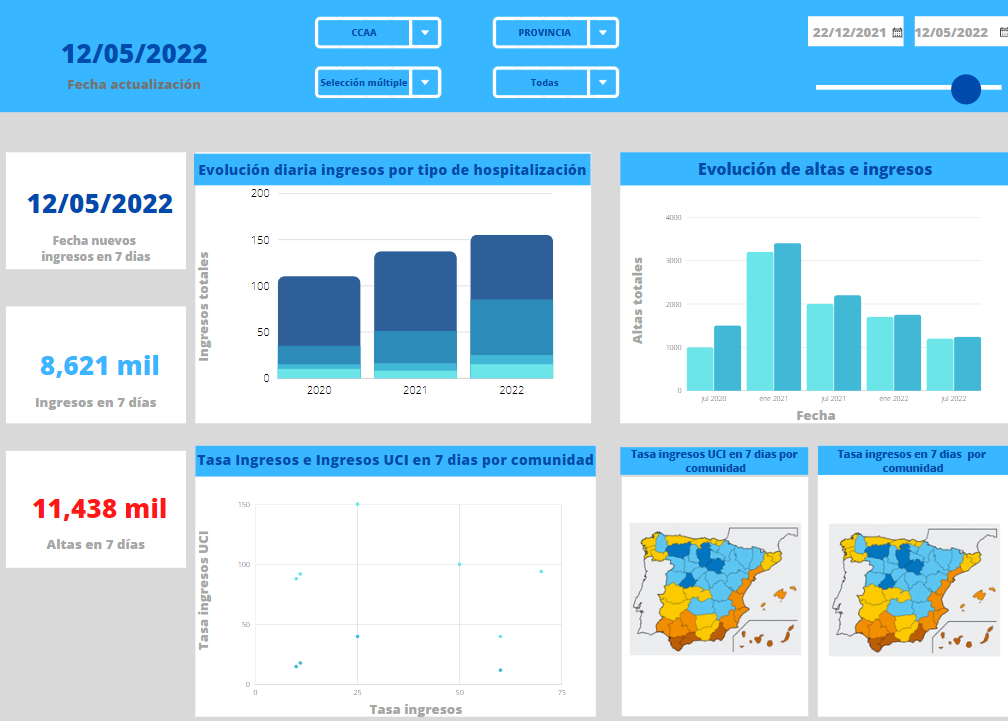
\includegraphics[scale=0.7]{img/prototipo_ingresosYaltas.PNG}
    \caption{Prototipo ingresos y altas hospitalarias.}
\end{figure}

Éste constaría de cuatro tarjetas con datos sobre fecha de actualización, la fecha de nuevos ingresos en 7 días, los ingresos en 7 días, y las altas en 7 días. 

También constaría de tres gráficos y dos mapas coropléticos, que facilitarían la visualización de información sobre la evolución diaria de ingresos por tipo de hospitalizaciones, la evolución de altas e ingresos, la tasa de ingresos y la tasa de ingresos UCI en 7 días por comunidad, la tasa de ingresos UCI en 7 días por comunidad, y la tasa de ingresos en 7 días por comunidad, respectivamente. 

Además, permitiría el filtrado de la información mediante filtros de fecha, comunidades autónomas y de provincia.

\newpage
A continuación, se incluye la interfaz final de los ingresos y altas hospitalarias. 

\begin{figure}[h]
    \advance\leftskip-0.5cm \rightskip5cm
    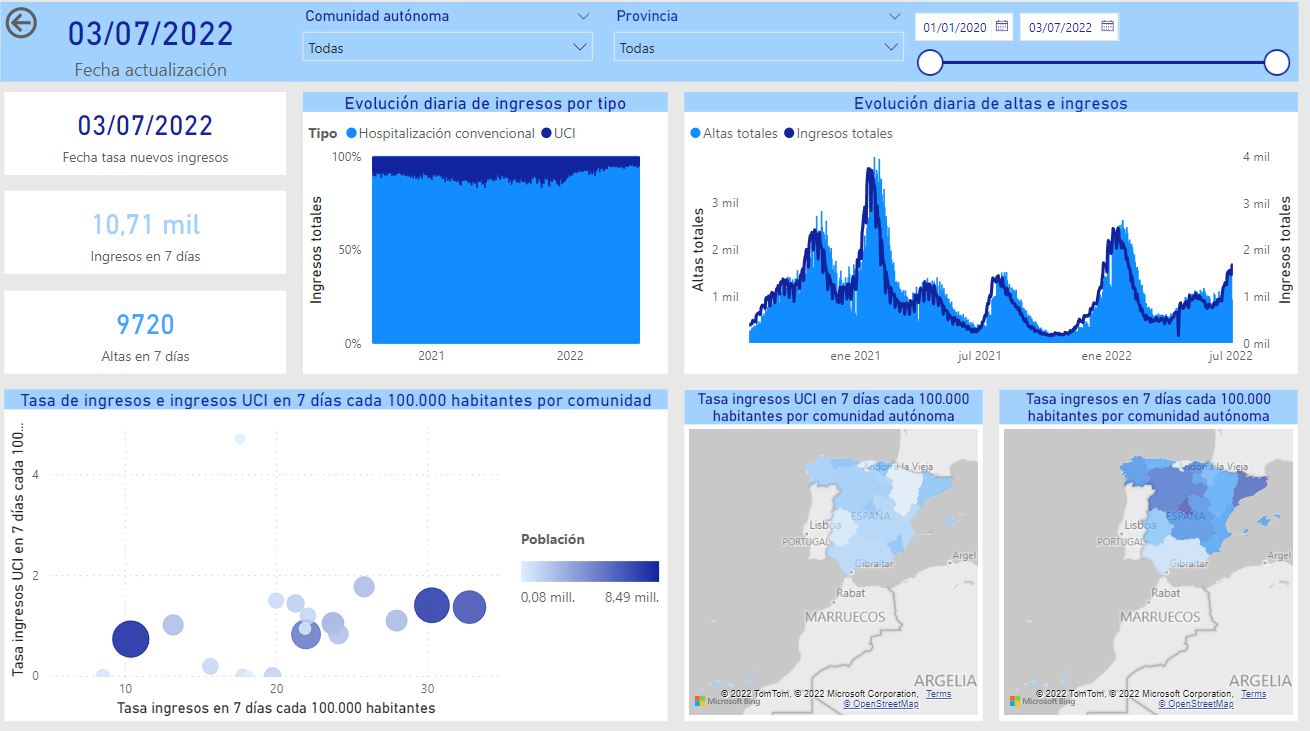
\includegraphics[scale=0.55]{img/powerBI_ingresosYaltas.PNG}
    \caption{Diseño ingresos y altas hospitalarias.}
\end{figure}

A pesar de que la interfaz final es muy similar al prototipo inicial, difieren en una serie de aspectos como en algunos títulos y tipos de gráficos.

\newpage
Seguidamente, se diseñó el prototipo de camas hospitalarias. 

\begin{figure}[h]
    \advance\leftskip-1cm \rightskip5cm
    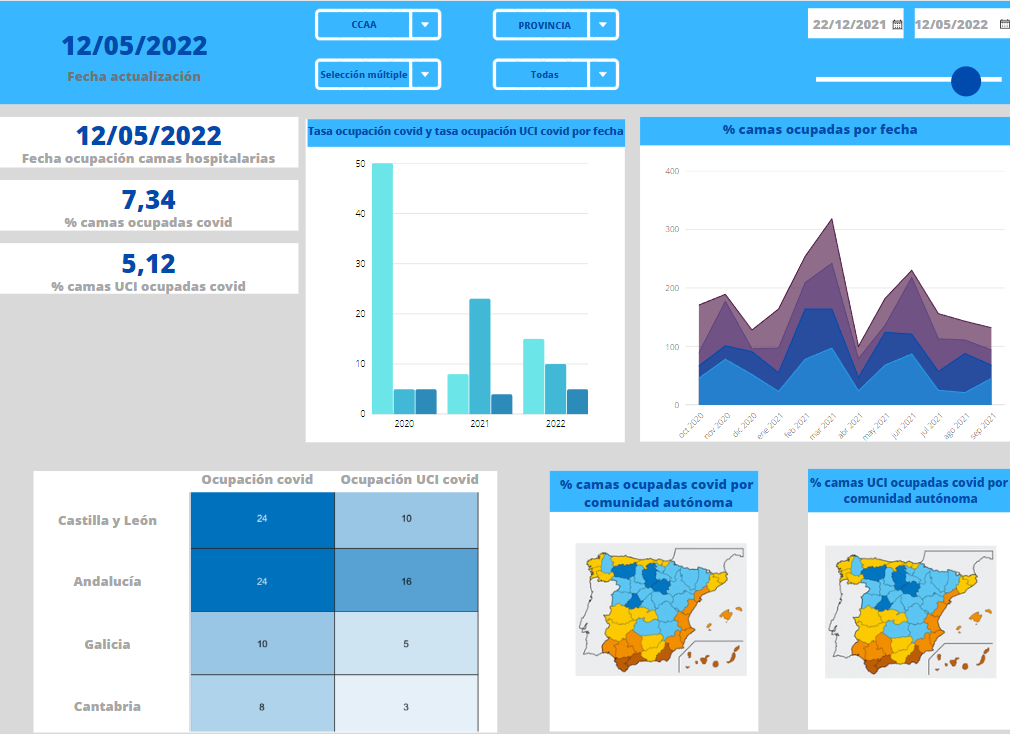
\includegraphics[scale=0.7]{img/prototipo_camas.PNG}
    \caption{Prototipo camas hospitalarias.}
\end{figure}

Éste constaría de cuatro tarjetas con datos sobre fecha de actualización, la fecha de ocupación de camas hospitalarias, el porcentaje de camas ocupadas por Covid-19, y el porcentaje de camas UCI ocupadas por Covid-19. 

También constaría de dos gráficos, una matriz y dos mapas coropléticos, que facilitarían la visualización de información sobre la tasa de ocupación covid y tasa de ocupación UCI por fecha, el porcentaje de camas ocupadas por fecha, la ocupación por Covid-19 y la ocupación UCI por Covid-19 por comunidades autónomas, el porcentaje de camas ocupadas por Covid-19 por comunidad autónoma, y el porcentaje de camas UCI ocupadas por Covid-19 por comunidad autónoma, respectivamente. 

Además, permitiría el filtrado de la información mediante filtros de fecha, comunidades autónomas y de provincia.

\newpage
A continuación, se incluye la interfaz final de las camas hospitalarias.

\begin{figure}[h]
    \advance\leftskip-0.5cm \rightskip5cm
    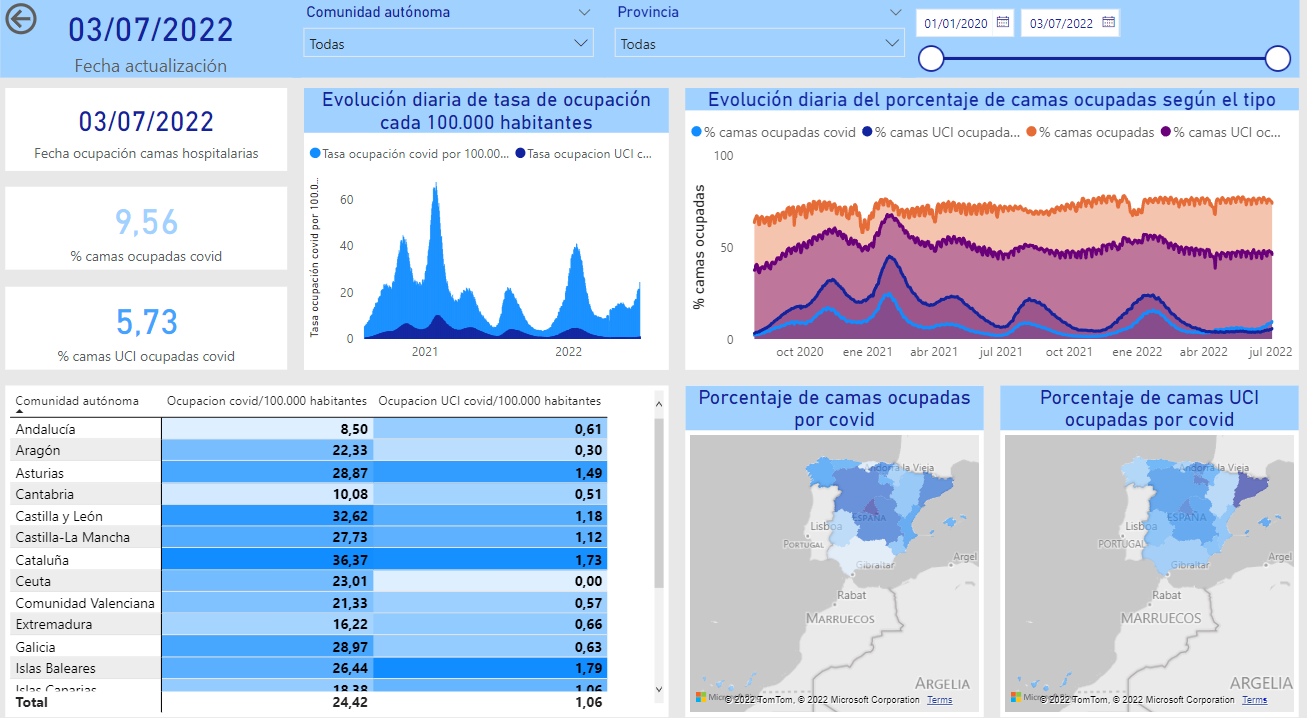
\includegraphics[scale=0.55]{img/powerBI_camas.PNG}
    \caption{Diseño camas hospitalarias.}
\end{figure}

A pesar de que la interfaz final es muy similar al prototipo inicial, difieren en una serie de aspectos como en algunos títulos y tipos de gráficos.

\newpage
Por último, se diseñó el prototipo de residencias. 

\begin{figure}[h]
    \advance\leftskip-1cm \rightskip5cm
    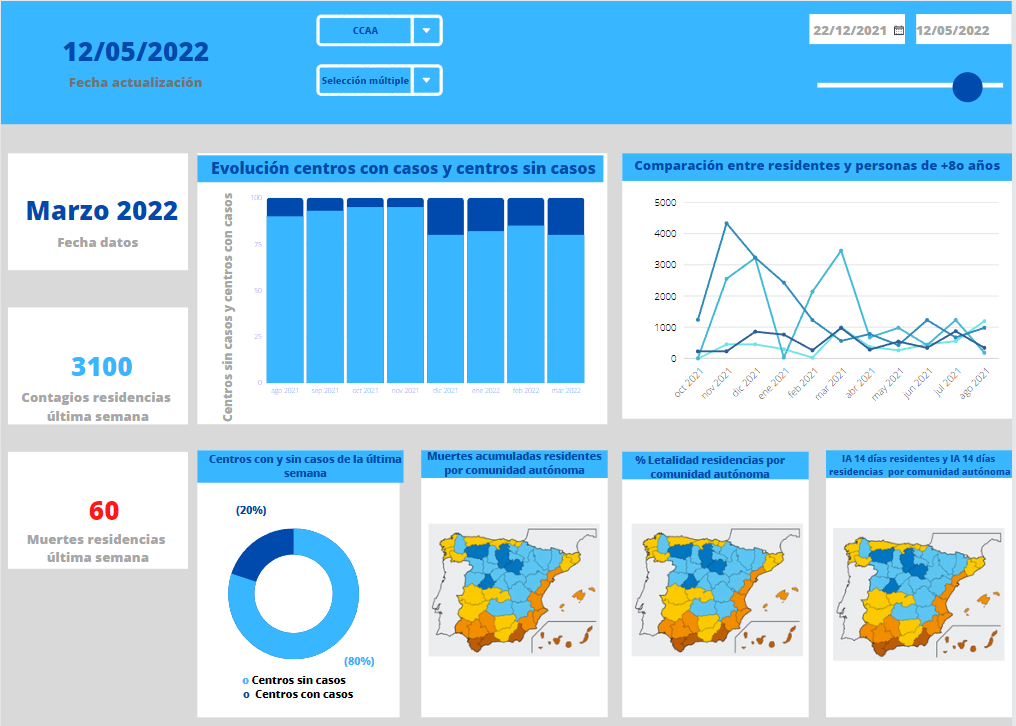
\includegraphics[scale=0.7]{img/prototipo_residencias.PNG}
    \caption{Prototipo residencias}
\end{figure}

Éste constaría de cuatro tarjetas con datos sobre la fecha de actualización, la fecha de los datos, los contagios en las residencias en la última semana, y las muertes en las residencias en la última semana. 

También constaría de tres gráficos y tres mapas coropléticos, que facilitarían la visualización de información sobre la evolución de los centros con casos y los centros sin casos, la comparación entre los residentes y personas de más de 80 años, los centros con casos y sin casos de la última semana, las muertes acumuladas de residentes  por comunidad autónoma, el porcentaje de letalidad de residentes por comunidad autónoma, y la incidencia acumulada a 14 días de los residentes por comunidad autónoma, respectivamente. 

Además, permitiría el filtrado de la información mediante un filtro de fecha y comunidades autónomas.

A continuación, se incluye la interfaz final de los ingresos y altas hospitalarias. 

\begin{figure}[h]
    \advance\leftskip-0.5cm \rightskip5cm
    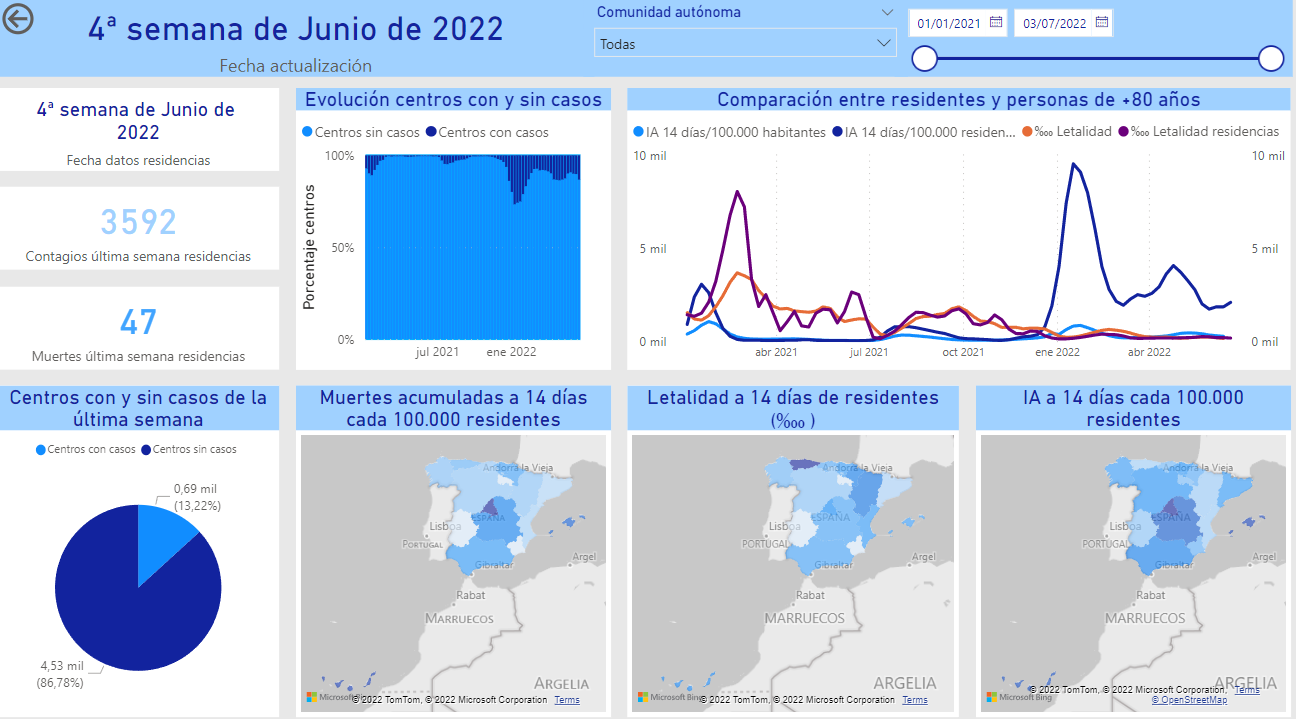
\includegraphics[scale=0.55]{img/powerBI_residencias.PNG}
    \caption{Diseño residencias}
\end{figure}

A pesar de que la interfaz final es muy similar al prototipo inicial, difieren en una serie de aspectos como algún título de gráfico.
\apendice{Documentación técnica de programación}

\section{Introducción}

\section{Estructura de directorios}

\section{Manual del programador}

\section{Compilación, instalación y ejecución del proyecto}

\section{Pruebas del sistema}

\apendice{Documentación de usuario}

\section{Introducción}

\section{Requisitos de usuarios}

\section{Instalación}

\section{Manual del usuario}





\bibliographystyle{plain}
\bibliography{bibliografiaAnexos}

\end{document}
